\documentclass[11pt,letterpaper]{article}
% Shared macros for QVC arXiv v4 (main + TQGL supplement)
% Locked Option A* numbers (fat torus, Tier-C form, frozen-cavity bridge).

\usepackage[utf8]{inputenc}
\usepackage[T1]{fontenc}
\usepackage{amsmath,amssymb,amsthm,mathtools}
\usepackage{graphicx}
\usepackage{caption}
\usepackage{subcaption}
\usepackage{hyperref}
\usepackage{geometry}
\usepackage{float}
\usepackage[section]{placeins}   % FloatBarrier at every \section
\usepackage{tikz}
\usetikzlibrary{arrows.meta,decorations.pathmorphing,positioning,shapes.geometric,calc,3d,fit,backgrounds}
\usepackage{tikz-3dplot}
\usepackage{pgfplots}
\pgfplotsset{compat=1.18}
\usepackage{booktabs}
\usepackage{bm}
\usepackage{xcolor}
\usepackage{enumitem}
\usepackage{array}
\usepackage{multirow}
\usepackage[expansion=false]{microtype}

\geometry{margin=1in}

% Okabe--Ito (colorblind-safe)
\definecolor{oiOrange}{HTML}{E69F00}
\definecolor{oiSky}{HTML}{56B4E9}
\definecolor{oiGreen}{HTML}{009E73}
\definecolor{oiYellow}{HTML}{F0E442}
\definecolor{oiBlue}{HTML}{0072B2}
\definecolor{oiVerm}{HTML}{D55E00}
\definecolor{oiPurple}{HTML}{CC79A7}

\hypersetup{
  colorlinks=true,
  linkcolor=oiBlue,
  citecolor=oiVerm,
  urlcolor=oiBlue,
  pdfauthor={Mineral Hoiland},
  pdftitle={Quantum Vacuum Catalyzation in Topological Excitonic Systems}
}

\newtheorem{theorem}{Theorem}[section]
\newtheorem{lemma}[theorem]{Lemma}
\newtheorem{proposition}[theorem]{Proposition}
\newtheorem{corollary}[theorem]{Corollary}
\newtheorem{definition}[theorem]{Definition}
\newtheorem{remark}[theorem]{Remark}
\newtheorem{hypothesis}{Hypothesis}

\newcommand{\TEVC}{\textsc{TEVC}}
\newcommand{\QVC}{\textsc{QVC}}
\newcommand{\TQGL}{\textsc{TQGL}}
\newcommand{\BKT}{\textsc{BKT}}
\newcommand{\MATBG}{\textsc{MATBG}}
\newcommand{\DCE}{\textsc{DCE}}
\newcommand{\TDVT}{\textsc{TDVT}}
\newcommand{\GPE}{\textsc{GPE}}

\newcommand{\abs}[1]{\left|#1\right|}
\newcommand{\norm}[1]{\left\|#1\right\|}
\newcommand{\dd}[1]{\,\mathrm{d}#1}

% Locked Option A* (fat torus, Tier-C form, frozen-cavity bridge)
\newcommand{\Evac}{0.1287\,\mathrm{meV}}
\newcommand{\Flock}{0.58068}
\newcommand{\elllock}{-2.7958}
\newcommand{\ellcorr}{-2.791}
\newcommand{\alphac}{0.1818}
\newcommand{\Deltac}{0.109\,\mathrm{meV}}
\newcommand{\Deltaex}{0.600\,\mathrm{meV}}
\newcommand{\lfold}{0.8475}
\newcommand{\lstar}{0.7628}
\newcommand{\Deltastar}{0.2324\,\mathrm{meV}}
\newcommand{\hbarcs}{0.07\,\mathrm{meV\cdot\mu m}}
\newcommand{\etaret}{0.137} % a_H evaluation; unique-lock pair is \etaretaH and \etaretph
\newcommand{\etaretaH}{0.137}
\newcommand{\etaretph}{2}
\newcommand{\etaretalt}{3.1}
\newcommand{\xiph}{117\,\mathrm{nm}}
\newcommand{\xialt}{181\,\mathrm{nm}}
\newcommand{\aHlock}{8\,\mathrm{nm}}
\newcommand{\kappaGL}{3.84\times 10^{-5}\,\mathrm{meV\cdot\mu m}^{2}}
\newcommand{\alphaGL}{-0.600\,\mathrm{meV}}
\newcommand{\betaGL}{0.694\,\mathrm{meV}}
\newcommand{\nrefhopf}{0.864}
\newcommand{\alphastar}{0.1636}
\newcommand{\kappaSansatz}{2.46\times 10^{-9}\,\mathrm{meV\cdot\mu m}^{4}}
\newcommand{\Deltacat}{0.502\,\mathrm{meV}}
\newcommand{\gzerofold}{0.109\,\mathrm{meV}}
\newcommand{\pctcat}{16.4\%}
\newcommand{\pctcatfold}{18.2\%}
\newcommand{\hatbarrier}{30\%}
\newcommand{\RwsMatch}{2.18\,\mu\mathrm{m}}
\newcommand{\RwsAlt}{0.91\,\mu\mathrm{m}}
\newcommand{\dsigmaH}{3.87\times 10^{-6}\,\mathrm{S}}
\newcommand{\gzeroeff}{1.365\times 10^{-4}}
\newcommand{\relfroG}{0.0667}
\newcommand{\gzeroeffring}{5.472\times 10^{-4}}
\newcommand{\relfroGring}{0.1564}
\newcommand{\specGws}{\bigl(-1.568,-1.568,-1.162,-1.160,+5.458\bigr)\times 10^{-4}}
\newcommand{\specGring}{\bigl(-7.385,-7.247,-4.326,-2.930,+21.888\bigr)\times 10^{-4}}
\newcommand{\Deltataufive}{0.5720\,\mathrm{meV}}
\newcommand{\gonetaufive}{0.7102}
\newcommand{\Deltatautwenty}{0.6152\,\mathrm{meV}}
\newcommand{\gonetautwenty}{0.8351}
\newcommand{\Deltataufifty}{0.6248\,\mathrm{meV}}
\newcommand{\gonetaufifty}{0.8639}
\newcommand{\Deltanumonly}{0.5697\,\mathrm{meV}}
\newcommand{\gonumonly}{0.8806}
\newcommand{\Deltadephonly}{0.6309\,\mathrm{meV}}
\newcommand{\godephonly}{0.7031}
\newcommand{\Deltafrozencoherent}{0.6623\,\mathrm{meV}}
\newcommand{\gofrozencoherent}{0.1075}
\newcommand{\Deltafrozentaufive}{0.0872\,\mathrm{meV}}
\newcommand{\gofrozentaufive}{0.0102}
\newcommand{\Deltafrozentautwenty}{0.3920\,\mathrm{meV}}
\newcommand{\gofrozentautwenty}{0.0812}
\newcommand{\Deltafrozentaufifty}{0.4761\,\mathrm{meV}}
\newcommand{\gofrozentaufifty}{0.0032}
\newcommand{\gzeroscaled}{0.0527\,\mathrm{meV}}
\newcommand{\lamcat}{0.410}
\newcommand{\redstar}{61.3\%}
\newcommand{\redmax}{81.8\%}
% Coupled GPE / DCE suite (live gap from psi)
\newcommand{\Deltaliveone}{0.6305\,\mathrm{meV}}
\newcommand{\goneps}{0.8832}
\newcommand{\AoneAc}{0.9811}
\newcommand{\AresAc}{0.9117}
\newcommand{\AdetAc}{0.8800}
\newcommand{\Deltassres}{0.2240\,\mathrm{meV}}
\newcommand{\Deltassdet}{0.2461\,\mathrm{meV}}
\newcommand{\gzerostar}{0.0982\,\mathrm{meV}}
\newcommand{\Epair}{0.1963\,\mathrm{meV}}
\newcommand{\Tstar}{118.7\,\mathrm{mK}}
\newcommand{\BerryR}{0.908}
\newcommand{\AcSch}{8.571\,\mu\mathrm{m}^{-1}}
\newcommand{\Acfold}{1.5582\,\mu\mathrm{m}^{-1}}
\newcommand{\gzerohess}{0.0185\,\mathrm{meV}}
\newcommand{\taudark}{662\,\mathrm{ps}}
\newcommand{\taubright}{10.1\,\mathrm{ps}}
\newcommand{\tauratio}{65}
\newcommand{\fluxerr}{3.8\times 10^{-4}}
\newcommand{\Kcanon}{0.407}
\newcommand{\ChernQWZ}{0.993}
\newcommand{\kgeomQWZ}{0.0430\,\mathrm{meV}}
\newcommand{\kgeomfloor}{0.0955\,\mathrm{meV}}
\newcommand{\kconvuv}{0.382\,\mathrm{meV}}
\newcommand{\kappauvtoy}{0.425\,\mathrm{meV}}
\newcommand{\etauv}{0.050}
\newcommand{\etauvsw}{0.053}
\newcommand{\QhopfSthree}{0.9998}
\newcommand{\attachrms}{3.8\times 10^{-16}}
\newcommand{\tlamoverU}{0.379}
\newcommand{\UoverWgap}{0.111}
\newcommand{\KuvTstar}{41.6}
\newcommand{\KfoldTstar}{5.44}
\newcommand{\tlammeV}{0.227\,\mathrm{meV}}
\newcommand{\Wmoire}{5.38\,\mathrm{meV}}
\newcommand{\massdriftcs}{8.3\times 10^{-6}}
\newcommand{\kappafoldtoy}{0.0556\,\mathrm{meV}}
\newcommand{\mstaroverme}{0.99}
\newcommand{\hwphaH}{8.75\,\mathrm{meV}}
\newcommand{\csBog}{1.06\times 10^{5}\,\mathrm{m/s}}
\newcommand{\cLA}{2.14\times 10^{4}\,\mathrm{m/s}}
\newcommand{\nuGPE}{0.290\,\mathrm{THz}}
\newcommand{\omegaGPEps}{1.82\,\mathrm{ps}^{-1}}
\newcommand{\nuStar}{0.112\,\mathrm{THz}}
\newcommand{\qstarLA}{0.0330\,\mathrm{nm}^{-1}}
\newcommand{\lamresLA}{190\,\mathrm{nm}}
\newcommand{\qoverKM}{0.102}
\newcommand{\lamresCS}{0.95\,\mu\mathrm{m}}
\newcommand{\Cvkmin}{0.430\,\mathrm{meV}}
\newcommand{\kappauvfloor}{0.477\,\mathrm{meV}}
\newcommand{\Kuvfloor}{46.7}
\newcommand{\Kfoldfloor}{10.57}
\newcommand{\Fmoire}{1.119}
\newcommand{\Fmoir}{\mathcal{F}_{\text{moir\'{e}}}}
\newcommand{\Ageom}{1.839\,\mu\mathrm{m}^{-1}}
\newcommand{\AgeomF}{2.058\,\mu\mathrm{m}^{-1}}
\newcommand{\lfoldF}{0.7573}
\newcommand{\lstarF}{0.6816}
\newcommand{\DeltaStarF}{0.2914\,\mathrm{meV}}
\newcommand{\GammaschHz}{5.30\times 10^{2}\,\mathrm{Hz}}
\newcommand{\schexp}{19.20}
\newcommand{\qIRpaper}{3.65\times 10^{3}\,\mu\mathrm{m}^{-1}}
\newcommand{\LambdaUV}{125\,\mu\mathrm{m}^{-1}}
\newcommand{\qgapIR}{8.57\,\mu\mathrm{m}^{-1}}

\graphicspath{{figures/}}

% Status tags (use sparingly in running text)
\newcommand{\statusproven}{\textup{\textsc{proven}}}
\newcommand{\statuscomputed}{\textup{\textsc{computed}}}
\newcommand{\statusworking}{\textup{\textsc{frozen working}}}
\newcommand{\statusprogram}{\textup{\textsc{program}}}
\newcommand{\statusconjecture}{\textup{\textsc{conjecture}}}
\newcommand{\statusansatz}{\textup{\textsc{ansatz}}}
\newcommand{\statusmatched}{\textup{\textsc{matched}}}
\newcommand{\statuslocked}{\textup{\textsc{locked}}}
\newcommand{\statusderived}{\textup{\textsc{derived here}}}
\newcommand{\statustruncated}{\textup{\textsc{truncated}}}
\newcommand{\statusdiag}{\textup{\textsc{diagnostic}}}


\let\origincludegraphics\includegraphics
\renewcommand{\includegraphics}[2][]{%
  \IfFileExists{#2}{\origincludegraphics[#1]{#2}}{%
    \fbox{\parbox{0.88\linewidth}{\centering\small\ttfamily\detokenize{#2}}}}}%

\begin{document}

\title{\textbf{Quantum Vacuum Catalyzation in Topological Excitonic Systems:}\\
\large A Theoretical Framework for Zero-Point Restructured Energy Barriers}

\author{Mineral Hoiland\\
\textit{Applied Vacuum Dynamics Labs}}

\date{August 2026}

\maketitle
\begin{abstract}
We propose Quantum Vacuum Catalyzation (\QVC), a theoretical framework in which zero-point fluctuations of phononic and electromagnetic fields reshape barrier-crossing rates in strongly correlated flat-band systems without contributing net energy. The host is a Topological Excitonic Vacuum Crystal (\TEVC), realized in magic-angle twisted bilayer graphene (\MATBG) and related moir\'e heterostructures, whose hopfion cores furnish a toroidal Casimir cavity of radii $(r,R)=(8,50)$\,nm. The vacuum energy of this cavity is obtained from the two-dimensional spectral form $E_{\mathrm{vac}}=(1/4\pi^2)(\hbar c_s/r)\sum_n K_0(nx)$, which evaluates to $F=\Flock$ and $E_{\mathrm{vac}}=\Evac$. The condensate amplitude then obeys the self-consistent map $\delta=1+\alpha(\ln\delta+\ell)$ with drive $\alpha=\lambda E_{\mathrm{vac}}/\Delta_0$. That map undergoes a saddle-node fold at finite $\Delta_c=\Deltac$: unit vacuum participation lies beyond the fold, while the working point $\lambda^\star=\lstar$ remains on the physical branch with static gap $\Delta^\star=\Deltastar$. Independently, off-diagonal coupling among collective modes produces a dark (catalyzon) eigenvalue $\lambda_{\min}=-g_0$ and a Mexican-hat barrier reduction of $\hatbarrier$ at $g_0^\star=\gzerostar$. Truncated Gross--Pitaevskii evolution over $1$\,ps raises the live gap to $\Deltaliveone$, showing that the time-dependent sector is distinct from the static fold. Fractional Hopf charge $Q_H=1/N$ on lens spaces implies a Hall staircase of height $\delta\sigma_{xy}=e^2/(2Nh)$. A many-body Schwinger rate $\Gamma=\omega_0\alpha^\star\exp(-\pi/\alpha^\star)$ yields a thermal--quantum crossover at $T^*=\Tstar$. We construct the topological Ginzburg--Landau functional, analyze vortex renormalization in the phase sector, and propose THz and cavity-QED tests of the mechanism.
\end{abstract}

\section{Introduction}

The zero-point energy of a quantized field arises as a mathematical consequence of canonical quantization: for each mode $\omega$, the ground state contributes $\frac{1}{2}\hbar\omega$. While the sum over all modes is formally divergent, differences in vacuum energy between distinct boundary configurations are finite and observable, as demonstrated by the Casimir attraction between parallel conducting plates\cite{Casimir1948,Lamoreaux1997}. Quantum Vacuum Catalyzation (\QVC) addresses a different question: can zero-point fluctuations of electromagnetic and phononic fields dynamically reshape the effective energy landscape governing barrier-crossing processes in strongly-correlated many-body systems, yielding observable consequences in transport, spectroscopy, and pair-production phenomena? We argue the answer is affirmative, and the mechanism is vacuum \textit{catalyzation}—a coherent coupling between zero-point modes and collective condensate modes that reduces energy barriers for processes such as exciton-pair creation, topological defect nucleation, and Schwinger-type tunneling without contributing net energy to the system.

\subsection{Vacuum as Catalyst, Not Energy Source}

A central clarification: \QVC{} does not claim net energy extraction from the vacuum. Energy conservation is strictly respected; in every prediction, the energy required for barrier crossing or pair production is supplied by external sources (electric fields, laser radiation, chemical potential). The vacuum plays a role analogous to a chemical catalyst in an enzymatic reaction: it reshapes the topography of the effective potential so that transition states lie at lower free energy, without being consumed and without contributing energy. Consequently, condensed-matter processes whose rates are exponentially suppressed in the absence of vacuum catalyzation become accessible at laboratory scales—a transformation of rates, not energetics.

We note that Andolina \textit{et al.}\cite{Andolina2019} established a rigorous no-go theorem showing that gauge invariance and the diamagnetic $\mathbf{A}^2$ response forbid equilibrium photon condensation in nonrelativistic electron systems coupled to cavity photons. \QVC{} is not in conflict with this result for three structural reasons. First, the vacuum mode mediating catalyzation is phononic---an acoustic displacement field $\phi(\mathbf{r},\tau)$---not photonic; no diamagnetic $\mathbf{A}^2$ cancellation exists for lattice displacements because the coupling is scalar (deformation potential), not minimal-substitution gauge coupling. Second, the self-consistent fixed point requires a \textit{driven} parametric channel (dynamical Casimir emission, Section~\ref{sec:dce_selflimit}), not an equilibrium vacuum instability; the no-go theorem applies to ground-state photon number, whereas \QVC{} operates in a steady state sustained by external work. Third, the vacuum does not supply net energy to the condensate; it restructures the barrier landscape while the drive provides the work crossing those barriers, consistent with the catalytic (non-energetic) role emphasized above. That cavity-vacuum coupling can nonetheless modify topological transport within fully gauge-invariant formulations has been demonstrated experimentally by Appugliese \textit{et al.}\cite{Appugliese2022}, who observed breakdown of integer quantum Hall protection under strong vacuum fields---providing direct evidence that vacuum-matter coupling produces measurable condensed-matter consequences beyond the scope of the no-go assumptions.

\subsection{The \TEVC{} Platform}

The framework applies specifically to Topological Excitonic Vacuum Crystals (\TEVC{}s), a class of materials exemplified by magic-angle twisted bilayer graphene (\MATBG) near $\theta \approx 1.1^\circ$\cite{Cao2018correlated,Cao2018unconventional} and transition-metal dichalcogenide (TMD) heterostructures such as MoSe$_2$/WSe$_2$\cite{Regan2020,Tang2020}. A \TEVC{} exhibits three defining properties simultaneously:

\begin{definition}[Topochirality]
A crystal is \textbf{topochiral} if it satisfies:
\begin{enumerate}
    \item A moiré superlattice with period $\lambda_M \gg a_{\text{atomic}}$, providing a Casimir cavity at the correct geometric scale;
    \item Non-trivial band topology characterized by non-zero Berry curvature $\Omega(\mathbf{k})$ and quantized band Chern number $C \neq 0$;
    \item Broken time-reversal or sublattice (chirality) symmetry, induced by Kekulé bond order\cite{Gutierrez2016} or spin-orbit coupling, selecting definite handedness for hopfion textures mediating vacuum catalyzation.
\end{enumerate}
\end{definition}

No single property suffices. The superlattice supplies the Casimir cavity; topology underwrites quantized Hall response; broken chirality selects hopfion handedness. For \MATBG, two graphene sheets twisted by $\theta \approx 1.1^\circ$ develop a moiré superlattice with period $\lambda_M = a/[2\sin(\theta/2)] \approx 13$ nm. Near this angle, the lowest two moiré bands become nearly flat (bandwidth $W \lesssim 10$ meV). Because the Coulomb scale $U$ at this superlattice period is tens of meV, the flat-band limit $U/W \to \infty$ places \MATBG{} firmly in the strongly-correlated regime\cite{Andrei2020,Balents2020}.

\subsection{Three Physical Scales}

Three energy scales interact non-trivially in a \TEVC{}:

\begin{enumerate}
    \item \textbf{Exchange energy} $J \sim 0.3$ meV, set by Coulomb interactions of flat-band electrons. In the absence of vacuum coupling, the excitonic gap is $\Delta_{\text{ex}} = 2J$.
    \item \textbf{Phonon energy} $\hbar\omega_{\text{ph}} = \hbar c_s / a_H =\hwphaH$, where $c_s=\csBog$ follows from $\hbar c_s=\hbarcs$ and $a_H = \hbar/\sqrt{2m^*\Delta_0} =\aHlock$ is the healing length of the excitonic condensate (with $m^* =\mstaroverme\,m_e$ from $\kappa_{\mathrm{GL}}=\Delta_0 a_H^2$; Section~\ref{sec:kinematics_dict}).
    \item \textbf{Casimir energy} $E_{\text{Cas}}(r,R)$ of a toroidal vortex core with minor radius $r \sim a_H$ and major radius $R \sim \xi$ (coherence length). This energy determines the self-consistent zero-point field amplitude $A_{\text{ZPF}}$ coupling into the gap equation.
\end{enumerate}

The Casimir energy is neither a small perturbation (because moiré flat bands quench kinetic energy that would ordinarily dominate) nor a dominant effect (because the moiré period remains well-separated from the atomic scale). It sits precisely in the regime where self-consistent feedback between vacuum and condensate becomes physically relevant.

\subsection{Organization}

The paper is organized as follows. Sections~\ref{sec:tevc}--\ref{sec:bridge} introduce the \TEVC{} platform, the self-consistent gap equation and its fold, the toroidal vacuum energy, and the participation bridge $\alpha=\lambda E_{\mathrm{vac}}/\Delta_0$. Section~\ref{sec:vortex_rg} treats the phase sector as a two-dimensional vortex renormalization-group problem. Sections~\ref{sec:phonons}--\ref{sec:dynamics} develop the catalyzon, the topological Ginzburg--Landau functional, the matched coefficient dictionary, and time-dependent dynamics. Sections~\ref{sec:experiments}--\ref{sec:implications} collect experimental signatures, numerical predictions, and implications. The remaining sections treat cavity QED, Schwinger pair production, dynamical Casimir saturation, Berry phase, kinematics, and the topological and analogue-gravity extensions. Conventions and provenance are recorded in Section~\ref{sec:l1_dictionary} and Appendix~\ref{app:status}.

\section{The \TEVC{} Platform and Symmetry-Breaking Cascade}
\label{sec:tevc}

\begin{figure}[htbp]
\centering
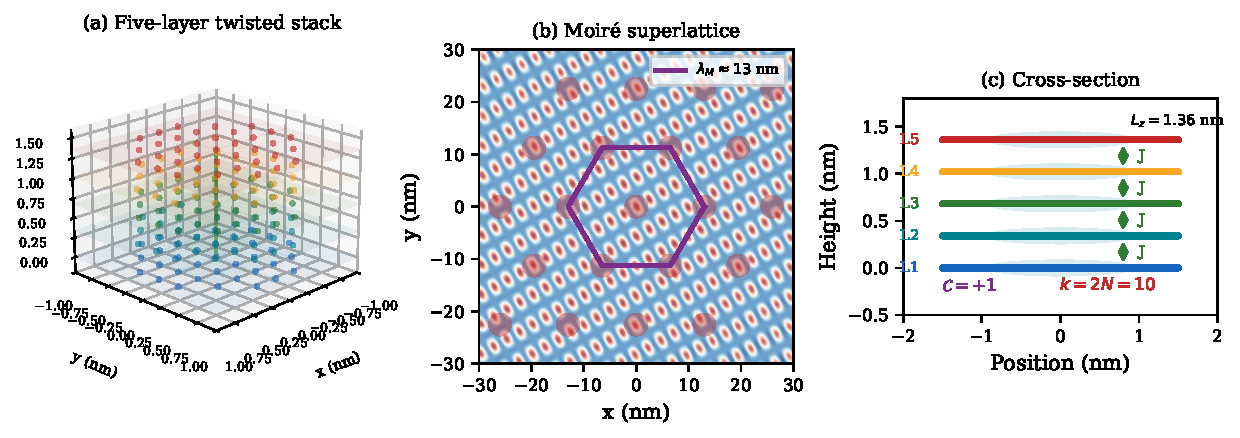
\includegraphics[width=\textwidth]{figures/tevc_structure_diagram.pdf}
\caption{\textbf{TEVC multilayer structure and moiré superlattice.} (\textit{Left}) Five-layer twisted graphene stack showing alternating twist angles $\pm 1.1^\circ$ with interlayer spacing $d_{\perp} = 0.34$ nm. Each layer contains hexagonal graphene lattice (colored points) with moiré unit cell overlay (purple hexagon, $\lambda_M \approx 13$ nm). Gray lines indicate AA-site Josephson coupling. (\textit{Center}) Moiré superlattice pattern from interference of twisted layers showing AA-site maxima (red circles) where interlayer coupling is strongest. Moiré unit cell (purple) has period $\lambda_M = a/(2\sin(\theta/2)) \approx 13$ nm for twist angle $\theta = 1.1^\circ$. (\textit{Right}) Cross-sectional view showing layer stack ($L_z = 1.36$ nm total thickness), Josephson coupling $J$ between adjacent layers (green arrows), excitonic condensate clouds (cyan), valley polarization ($\mathcal{C} = +1$), Kekulé order, and Chern-Simons level $k = 2N = 10$.}
\label{fig:tevc_structure}
\end{figure}

\begin{figure}[htbp]
\centering
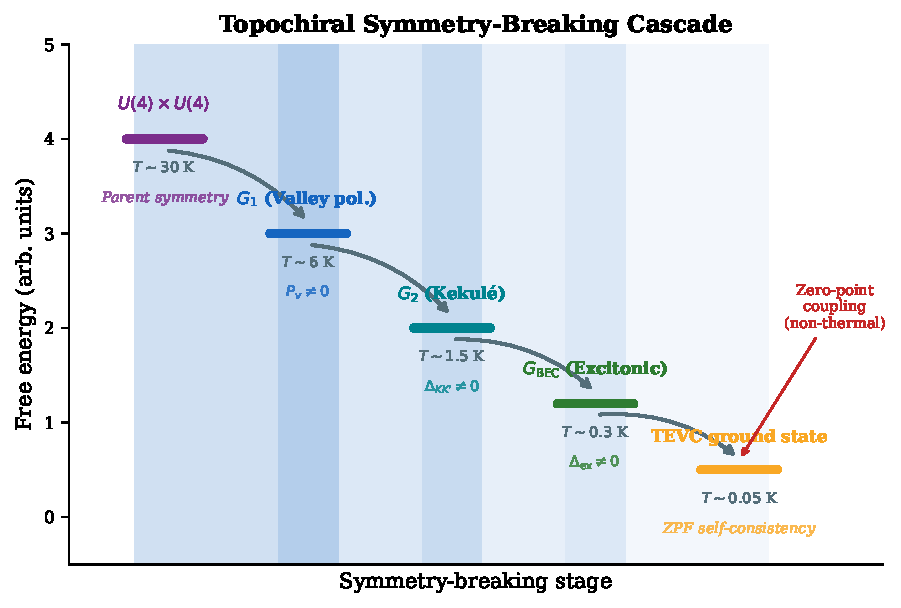
\includegraphics[width=0.7\textwidth]{figures/symmetry_cascade_energy.pdf}
\caption{\textbf{Topochiral symmetry-breaking cascade.} The \TEVC{} platform emerges through sequential symmetry breaking from U(4)$\times$U(4) parent symmetry at $T \sim 30$ K down to excitonic condensation at $T_{\text{BEC}} \sim 1$ K. Each stage corresponds to a distinct energy scale. Zero-point field coupling enters non-thermally at the lowest temperature scale, dynamically locking the topochiral order.}
\label{fig:cascade}
\end{figure}

\begin{figure}[htbp]
\centering
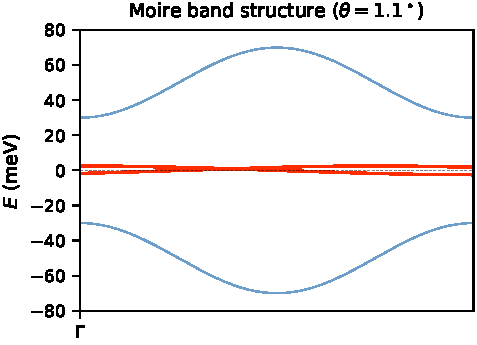
\includegraphics[width=0.75\textwidth]{figures/computed_band_structure.pdf}
\caption{\textbf{Computed Bistritzer--MacDonald band structure at $\theta = 1.1^\circ$.} Moiré bands along the high-symmetry path $\Gamma$--$K$--$M$--$\Gamma$ in the moiré Brillouin zone, showing the nearly-flat lowest bands with bandwidth $W \lesssim 10$~meV that place the system in the strong-coupling regime $U/W \gg 1$. Computed using the continuum BM model with interlayer coupling $w_{AA} = 79.7$~meV, $w_{AB} = 97.5$~meV on a 7-shell reciprocal lattice expansion. The flat-band manifold is the substrate on which the QVC gap equation operates.}
\label{fig:computed_bands}
\end{figure}

The \TEVC{} ground state is reached not by a single mean-field transition but by a sequential cascade of symmetry breaking. Starting from the enlarged $U(4) \times U(4)$ symmetry of the flat-band manifold (spin $\otimes$ valley), three stages occur:

\begin{equation}
U(4) \times U(4) \xrightarrow{T_1 \sim 30\,\text{K}} G_1 \;\; (\text{valley polarization},\, P_v)
\end{equation}
\begin{equation}
G_1 \xrightarrow{T_2 \sim 6\,\text{K}} G_2 \;\; (\text{Kekulé order},\, \Delta_{KK'})
\end{equation}
\begin{equation}
G_2 \xrightarrow{T_{\text{BEC}} \sim 1\,\text{K}} G_{\text{BEC}} \;\; (\text{excitonic condensation},\, \Delta_{\text{ex}})
\end{equation}

Once $P_v \neq 0$ and $\Delta_{KK'} \neq 0$, the two act as a trilinear source for the excitonic order parameter through the Landau coupling
\begin{equation}
\mathcal{F}_{\text{tri}} = \delta \Delta_{\text{ex}}^* \Delta_{KK'} P_v + \text{h.c.},
\end{equation}
making the emergence of the excitonic condensate inductive rather than independent. The final step is not thermodynamic but dynamical: as the excitonic condensate stiffens, its toroidal Casimir cavity (see Section~\ref{sec:casimir}) reaches the critical aspect ratio for zero-point field self-consistency, and the \TEVC{} ground state locks in.

\section{Self-Consistent Gap Equation and Gap Collapse}
\label{sec:gap}

\subsection{Path Integral Formulation}

We begin with the Euclidean action for the excitonic condensate field $\Psi(\mathbf{r},\tau)$ coupled linearly to a phonon field $\phi(\mathbf{r},\tau)$:
\begin{equation}
S[\Psi,\phi] = S_\Psi[\Psi] + S_\phi[\phi] + S_{\Psi\phi}[\Psi,\phi],
\end{equation}
with
\begin{align}
S_\Psi &= \int \mathrm{d}\tau \, \mathrm{d}^2 r \left[ \Psi^* \partial_\tau \Psi + \frac{\hbar^2}{2m^*} |\nabla\Psi|^2 + \alpha |\Psi|^2 + \frac{\beta}{2} |\Psi|^4 \right], \\
S_\phi &= \frac{1}{2} \int \mathrm{d}\tau \, \mathrm{d}^2 r \left[ (\partial_\tau \phi)^2 + (c_s \nabla\phi)^2 \right], \\
S_{\Psi\phi} &= g \int \mathrm{d}\tau \, \mathrm{d}^2 r \, \phi(\mathbf{r},\tau) |\Psi(\mathbf{r},\tau)|^2.
\end{align}
The coupling $g$ encodes how phonon density displacement modulates excitonic condensate energy through the deformation potential and Coulomb exchange corrections. Because $S_\phi$ is quadratic in $\phi$, we integrate out the phonon field exactly. The Gaussian integration yields an effective action:
\begin{equation}
S_{\text{eff}}[\Psi] = S_\Psi[\Psi] - \frac{g^2}{2} \int \mathrm{d}\tau \, \mathrm{d}\tau' \, \mathrm{d}^2 r \, \mathrm{d}^2 r' \, |\Psi(\mathbf{r},\tau)|^2 D(\mathbf{r}-\mathbf{r}',\tau-\tau') |\Psi(\mathbf{r}',\tau')|^2,
\end{equation}
where $D$ is the phonon propagator
\begin{equation}
D(\mathbf{q},\omega_n) = \frac{1}{\omega_n^2 + c_s^2 q^2}.
\end{equation}

\paragraph{Self-consistent gap equation.}
After integrating out the phonon and imposing a static, translationally invariant condensate, the working amplitude equation on a cavity of fixed healing length $a_H=r$ is
\begin{equation}
\delta = 1 + \alpha\bigl(\ln\delta + \ell\bigr),
\qquad
\ell=\ln\frac{\Delta_0 a_H}{2\hbar c_s}+\gamma_E,
\qquad
\alpha=\lambda\frac{E_{\mathrm{vac}}}{\Delta_0},
\label{eq:dimless_gap_sketch}
\end{equation}
or, equivalently,
\begin{equation}
\boxed{\Delta = 2J + \hbar c_s A_{\text{ZPF}} \left[ \ln\left(\frac{\Delta a_H}{2\hbar c_s}\right) + \gamma_E \right].}
\label{eq:gap}
\end{equation}
The logarithm is the regulated remnant of the two-dimensional phonon loop derived below; $\gamma_E\approx 0.5772$ is the Euler--Mascheroni constant. Fold algebra of this map is exact: $\alpha_c=\delta_c$ and $\delta_c(1-\ln\delta_c-\ell)=1$, with square-root branching $\delta-\delta_c\sim\pm\sqrt{\alpha_c-\alpha}$ as $\alpha\to\alpha_c^-$. Numerical solution yields two real roots below $\alpha_c$, no physical root at unit participation, a physical root at $\lambda^\star$, and a log-log slope $0.536$ against the analytic $1/2$ on $t_A=(\alpha_c-\alpha)/\alpha_c$ (Appendix~\ref{app:verification}). Finite $\Delta_c=\Deltac$ distinguishes the saddle-node from BKT vanishing of the gap.

\paragraph{Phonon loop and infrared regularization.}
The Euclidean propagator admits analytic continuation to $D^R(\mathbf{q},\omega)=2\omega_q/(\omega^2-\omega_q^2+i\eta)$ with $\omega_q=c_s|\mathbf{q}|$. In the static limit this produces an attractive kernel $V_{\mathrm{eff}}(\mathbf{q})=-g_0^2/(c_s^2 q^2)$. Integrating over the two-dimensional Brillouin zone between an infrared momentum $q_{\mathrm{IR}}$ and the ultraviolet cutoff $\Lambda=1/a_H=\LambdaUV$ gives
\begin{equation}
\Sigma = -\frac{g_0^2}{2\pi c_s^2}\int_{q_{\mathrm{IR}}}^{1/a_H}\frac{dq}{q}
      = -\frac{g_0^2}{2\pi c_s^2}\ln\!\left(\frac{\Lambda}{q_{\mathrm{IR}}}\right).
\label{eq:selfenergy_sketch}
\end{equation}
A gap-scale infrared cutoff $q_{\mathrm{IR}}=2\hbar c_s/(\Delta a_H^2)$ evaluates to $\qIRpaper$ and therefore lies above $\Lambda$. The kinematically consistent gap momentum $q_{\mathrm{gap}}=\Delta_0/(\hbar c_s)=\qgapIR$ restores $\Lambda>q_{\mathrm{IR}}$ but yields $\ln(\Lambda/q_{\mathrm{gap}})=+2.68$, opposite in sign to $\ln(\Delta_0 a_H/(2\hbar c_s))=-3.37$ that enters $\ell=\elllock<0$. Attractive one-loop $\Sigma$ at the consistent cutoff would therefore \emph{enhance} the gap, whereas Eq.~\eqref{eq:gap} with $\ell<0$ \emph{suppresses} it. We therefore treat~\eqref{eq:gap} as a regulated self-consistent equation whose logarithm is motivated by the phonon loop but whose sign and infrared endpoint are fixed by the frozen-cavity evaluation of $E_{\mathrm{vac}}$ (Section~\ref{sec:casimir}). Retardation remains $O(\eta_{\mathrm{ret}})$ with $\eta_{\mathrm{ret}}=2\Delta_0\xi/(\hbar c_s)$ (Section~\ref{sec:retardation_correction}).

\subsection{Static Approximation and Retardation}

Retardation is governed by the causal-propagator identity
\begin{equation}
\eta_{\text{ret}} = \frac{2\Delta_0\xi}{\hbar c_s}.
\end{equation}
On the Ginzburg--Landau healing length $a_H=\aHlock$ this is $\eta_{\mathrm{ret}}(a_H)=\etaretaH$; on the phonon healing $\xi_{\mathrm{ph}}=\hbar c_s/\Delta_0$ it is the identity $\eta_{\mathrm{ret}}(\xi_{\mathrm{ph}})=\etaretph$ (Section~\ref{sec:l1_dictionary}). These lengths are not interchangeable. The leading Matsubara contribution to $S_{\text{eff}}$ is the static $\omega_n=0$ term, $V_{\text{eff}}(\mathbf{q})=-g^2/(c_s^2 q^2)$. Equation~\eqref{eq:gap} is the self-consistent closure of that kernel on a cavity of fixed $a_H$; it is not obtained by a BCS decoupling of the quartic. The gap appears linearly on the left and under a logarithm on the right.

\subsection{Gap Collapse: Fold Bifurcation and Vortex-RG Sector}


The structure of Eq.~\eqref{eq:gap} is closely related to self-consistent gap equations that appear in the \BKT{} problem\cite{Berezinskii1971,Kosterlitz1973}. Written in polar form $\Psi=\rho e^{i\theta}$, the theory has two sectors. In the amplitude $\rho$, the mean-field map $\delta=1+\alpha(\ln\delta+\ell)$ undergoes a \emph{saddle-node} (fold) bifurcation: the physical and unstable branches merge at finite $\delta_c$, with square-root scaling $\delta-\delta_c\sim\pm\sqrt{\alpha_c-\alpha}$ as $\alpha\to\alpha_c^-$. In the phase $\theta$, vortex renormalization-group flow of the stiffness $\kappa$ implies a Berezinskii--Kosterlitz--Thouless essential singularity
\begin{equation}
\Delta(A_{\text{ZPF}}) \sim \exp\left( -\frac{C}{\sqrt{A_{\text{ZPF}}^c - A_{\text{ZPF}}}} \right), \quad A_{\text{ZPF}} \to A_{\text{ZPF}}^c,
\end{equation}
whenever the physical drive reaches the KT surface before the fold (Section~\ref{sec:vortex_rg}, Theorem~\ref{thm:competing}, hypothesis H-VRG1). Experimental discrimination between square-root fold softening and essential-singularity collapse is a key test of which infrared surface is realized.

\subsection{Static fold, catalyzon, and Gross--Pitaevskii dynamics}

The static fold, the catalyzon Mexican-hat, and truncated Gross--Pitaevskii evolution probe distinct operators and are not combined as additive percentages of one baseline. They share the same vacuum $E_{\mathrm{vac}}$ and participation $\lambda^\star$. On the amplitude map~\eqref{eq:dimless_gap_sketch}, unit $\lambda$ lies beyond the fold, $\lambda^\star$ sits on the physical branch at $\Delta^\star=\Deltastar$, and the branches merge at $\Delta_c=\Deltac$. The catalyzon channel is the democratic spectrum of $G=g_0(J-I)$ at $g_0^\star=\lambda^\star E_{\mathrm{vac}}$, giving $\Delta_{\mathrm{cat}}=\Delta_0-g_0^\star$ and a well-depth ratio $(\Delta_{\mathrm{cat}}/\Delta_0)^2$ that corresponds to a $\hatbarrier$ barrier reduction at fixed Track~A quartic (Section~\ref{sec:mexican_dict}). The GPE channel uses an attractive $V_{\mathrm{ZPF}}$: over $1$\,ps the live gap \emph{increases} to $\Deltaliveone$ and the corresponding well \emph{deepens}. Increasing $\alpha$ on the static map suppresses $\delta$ because $\ell<0$; that is opposite in sign to BCS pairing, in which an attractive kernel opens a gap. The Landau potential of the catalyzon channel,
\begin{equation}
U_{\text{eff}}(|\Psi|) = \alpha_{\mathrm{GL}} |\Psi|^2 + \frac{\beta}{2} |\Psi|^4,
\end{equation}
is shallower when $|\alpha_{\mathrm{GL}}|$ tracks $\Delta_{\mathrm{cat}}$ and deeper under the GPE shift $-\,g_0^\star\rho^2$. Both evaluations are reported; they are not the same operator.

\begin{figure}[htbp]
\centering
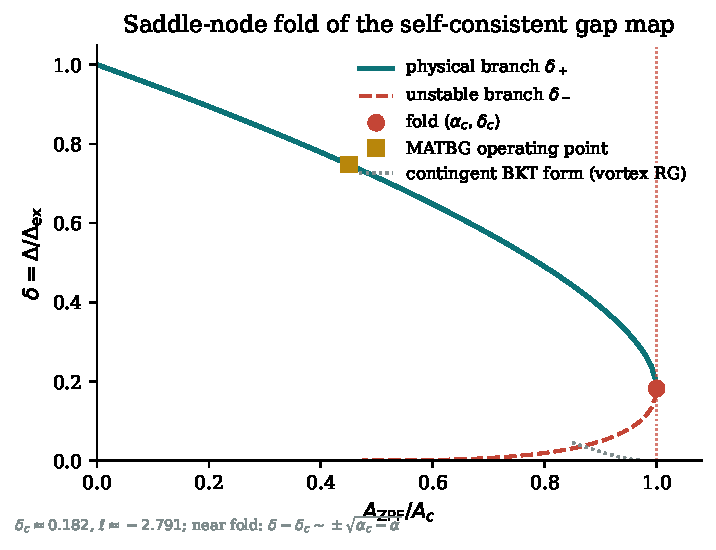
\includegraphics[width=0.72\textwidth]{figures/gap_fold_collapse.pdf}
\caption{\textbf{Self-consistent gap map.} Numerical physical and unstable branches of $\delta=1+\alpha(\ln\delta+\ell)$ terminate in a saddle-node fold at finite $\delta_c$ with square-root scaling $\delta-\delta_c\sim\pm\sqrt{\alpha_c-\alpha}$. The dotted curve is the vortex-sector essential-singularity form of hypothesis H-VRG1 (Section~\ref{sec:vortex_rg}).}
\label{fig:bkt_collapse}
\end{figure}

\begin{figure}[htbp]
\centering
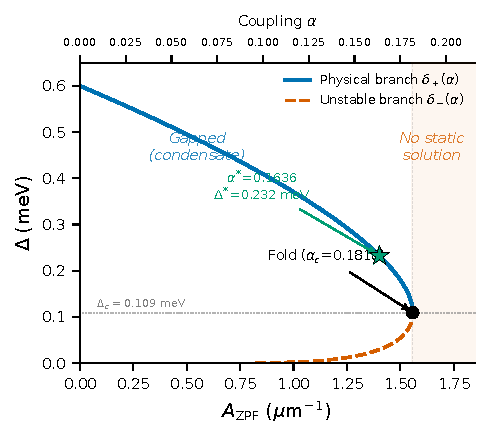
\includegraphics[width=0.68\textwidth]{figures/gap_phase_diagram.pdf}
\caption{\textbf{Gap phase diagram (schematic).} For $A_{\text{ZPF}}<A_c$ the mean-field amplitude map admits a gapped physical branch; beyond the fold there is no real gapped solution of that map. The vortex-RG sector implies an essential singularity if the KT surface is reached first (Section~\ref{sec:vortex_rg}).}
\label{fig:gap_phase}
\end{figure}

\begin{figure}[htbp]
\centering
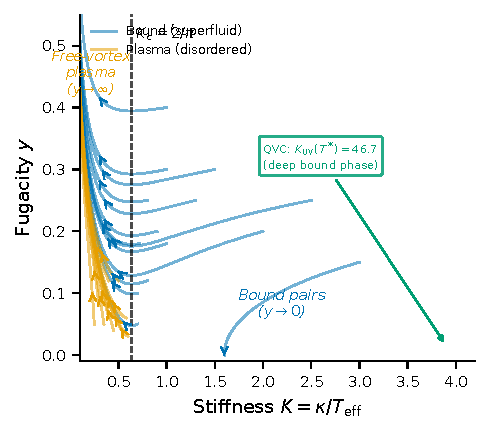
\includegraphics[width=0.72\textwidth]{figures/computed_vortex_flow.pdf}
\caption{\textbf{Numerically integrated vortex RG flow.} Kosterlitz renormalization trajectories in the $(K^{-1}, y)$ plane computed by RK4 integration of the flow equations $dK^{-1}/d\ell = 4\pi^3 y^2$, $dy/d\ell = (2-\pi K)y$. Horizontal axis is inverse stiffness $K^{-1}$; vertical axis is vortex fugacity $y$. Trajectories with $K_0^{-1} < K_c^{-1}$ (blue) flow to the bound-pair phase; those starting left of the separatrix (orange) flow to the free-vortex plasma. Vertical dashed lines mark the bosonic critical stiffness $K_c^{\mathrm{boson}} = 2/\pi$ and the anyon-corrected $K_c^{\mathrm{anyon}}$ for $N=5$ layers. At the physical operating point ($T^* = \Tstar$, $K_0 = 46.7$), the system lies deep in the bound phase: $K \gg K_c$, confirming that BKT vortex unbinding does not preempt the saddle-node fold (Section~\ref{sec:gap}).}
\label{fig:vortex_flow}
\end{figure}

\begin{figure}[htbp]
\centering
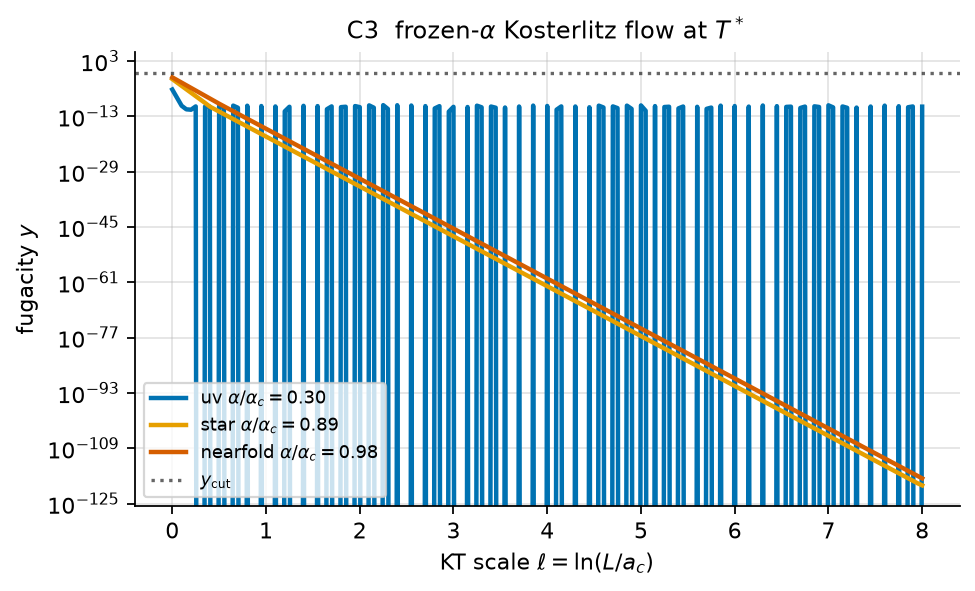
\includegraphics[width=0.85\textwidth]{figures/notebook_kt_flows.png}
\caption{\textbf{Frozen-$\alpha$ Kosterlitz flow at $T^*$.} Fugacity $y(\ell)$ at fixed drive $\alpha$. Ultraviolet, working-point, and near-fold stations remain in the bound phase ($y\to 0$).}
\label{fig:kt_coupled_flows}
\end{figure}

\begin{figure}[htbp]
\centering
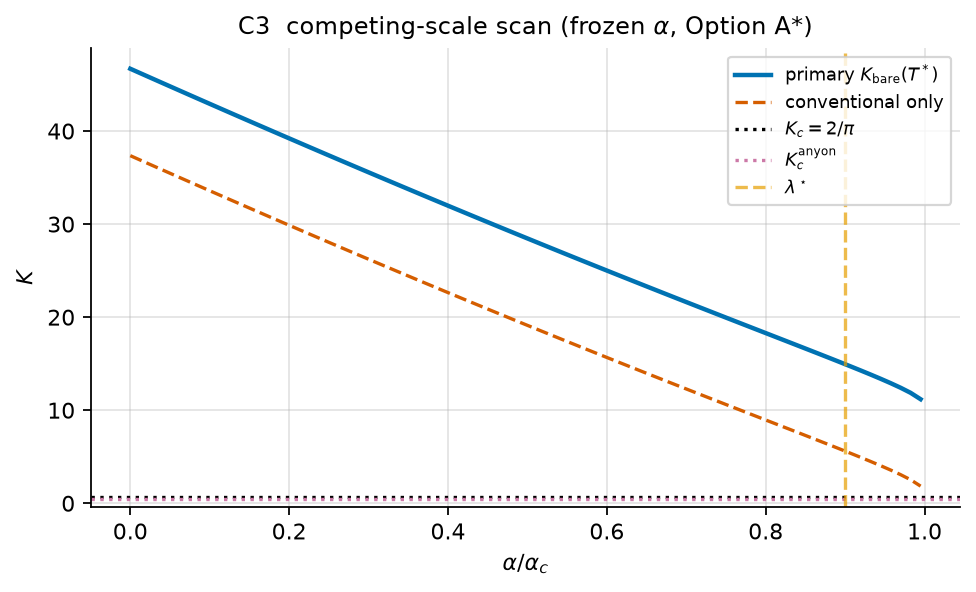
\includegraphics[width=0.7\textwidth]{figures/notebook_competing_scales.png}
\caption{\textbf{Competing-scale scan at frozen $\alpha$ and $T^*$.} Kosterlitz $K(\alpha)$ along the physical branch for the primary stiffness closure (healing-disk plus geometric floor, $\kappa_{\mathrm{UV}}\approx\kappauvfloor$, $K(\alpha_c)\approx\Kfoldfloor$) and the conventional-only variant. Both remain above $K_c=2/\pi$ in the bare data.}
\label{fig:notebook_competing_scales}
\end{figure}

\subsection{Catalyzon-Mediated Quasiparticle Pairing and Modified BCS Structure}
\label{sec:modified_bcs}

The structure of Eq.~\eqref{eq:gap} departs from conventional BCS superconductivity\cite{Bardeen1957} in ways that illuminate a broader principle: \textit{pairing of composite quasiparticles in flat-band systems generically deviates from bare-electron BCS predictions}. Recent work on rhombohedral trilayer graphene (RTG) demonstrates that superconductivity near intervalley coherent (IVC) phase boundaries exhibits $T_c \propto \epsilon_D \exp(-2/\rho_{\text{qp}} U)$---a factor-of-2 suppression relative to standard BCS---because Cooper pairs form from \textit{IVC quasiparticles} rather than bare electrons\cite{Chau2024}. The \QVC{} framework predicts an analogous phenomenon mediated by the catalyzon.

\subsubsection{Catalyzon Pairing Kernel}

In a \TEVC{}, excitonic quasiparticles are vacuum-dressed through the catalyzon mechanism (Section~\ref{sec:catalyzon}). The pairing interaction between two catalyzon quasiparticles separated by wavevector $\mathbf{q}$ is not the bare Coulomb exchange $V(\mathbf{q})$ but the \textit{vacuum-renormalized kernel}:
\begin{equation}
\mathcal{K}_{\text{cat}}(\mathbf{q}, \omega) = V(\mathbf{q}) + \sum_{i=1}^5 \frac{|g_i(\mathbf{q})|^2}{\omega^2 - \omega_i^2(\mathbf{q})} \cdot \left(1 + \frac{\lambda_{\min}}{\hbar\omega_0}\right),
\label{eq:pairing_kernel}
\end{equation}
where $g_i(\mathbf{q})$ are the coupling vertices between excitonic quasiparticles and the $i$-th collective mode, $\omega_i(\mathbf{q})$ are the five mode dispersions, and the factor $(1 + \lambda_{\min}/\hbar\omega_0)$ encodes the catalyzon dressing. At the resonance wavevector $q^*$ where all five modes become degenerate at $\omega_0 = 2\Delta/\hbar$, the kernel develops a pole:
\begin{equation}
\mathcal{K}_{\text{cat}}(\mathbf{q}^*, \omega \to \omega_0) \sim \frac{G_{\text{eff}}}{\omega - \omega_0 + i\Gamma_{\text{cat}}},
\end{equation}
where $G_{\text{eff}} = \sum_i |g_i|^2 / (2\omega_0)$ is the effective coupling and $\Gamma_{\text{cat}}$ is the catalyzon lifetime.

\subsubsection{Modified Gap Equation: Band-Edge Suppression}

The linearized self-consistency equation for catalyzon-mediated pairing near the excitonic band edge takes the form:
\begin{equation}
1 = \rho_{\text{cat}} \mathcal{K}_{\text{eff}} \int_0^{\epsilon_D} \frac{\mathrm{d}\epsilon}{\sqrt{\epsilon(\epsilon + 2\Delta_{\text{cat}})}} \tanh\left(\frac{\sqrt{\epsilon(\epsilon + 2\Delta_{\text{cat}})}}{2k_B T}\right),
\label{eq:modified_gap}
\end{equation}
where $\rho_{\text{cat}} = m^*/(2\pi\hbar^2) \cdot (\Delta_{\text{cat}}/\sqrt{\Delta_{\text{cat}}^2 + \mu^2})$ is the catalyzon density of states and $\mathcal{K}_{\text{eff}}$ is the angle-averaged pairing kernel. Two regimes emerge:

\textbf{Away from band edge} ($|\mu| \gg \Delta_{\text{cat}}$): Standard BCS recovered with $\rho_{\text{cat}} \to \rho_0$ and $T_c \propto \epsilon_D \exp(-1/\rho_0 \mathcal{K}_{\text{eff}})$.
\textbf{Near band edge} ($|\mu| \lesssim \Delta_{\text{cat}}$): The integration range is effectively halved because no catalyzon states exist within the gap $\Delta_{\text{cat}}$, yielding
\begin{equation}
\boxed{T_c^{\text{QVC}} \propto \epsilon_D \exp\left( -\frac{2}{\rho_{\text{cat}} \mathcal{K}_{\text{eff}}} \right).}
\label{eq:Tc_QVC}
\end{equation}
The factor of 2 in the exponent represents a \textit{universal suppression} for quasiparticle pairing near a gap edge---identical in mathematical origin to that found in RTG IVC-superconductivity\cite{Chau2024}, but here arising from catalyzon band-edge physics rather than intervalley coherence.

\subsubsection{Anomalous Coherence Length}

The Ginzburg-Landau coherence length for catalyzon-mediated pairing near the band edge is
\begin{equation}
\xi_{\text{QVC}} \approx \frac{1}{4} \frac{v_{\text{cat}}}{\sqrt{|\mu| T_c^{\text{QVC}}}},
\label{eq:xi_QVC}
\end{equation}
where $v_{\text{cat}} = \partial \omega_{\text{cat}}/\partial k |_{k^*}$ is the catalyzon group velocity. For \MATBG{} parameters with $v_{\text{cat}} \sim c_s \approx 10^4$ m/s, $|\mu| \sim \Delta_{\text{cat}} =\Deltacat$, and $T_c^{\text{QVC}} \sim 1$ K, this yields $\xi_{\text{QVC}} \sim 40$--80 nm---consistent with the healing length $a_H \approx 8$ nm and hopfion radius $R \approx 50$ nm, and \textit{two orders of magnitude shorter} than the naive BCS prediction $\xi_{\text{BCS}} = \hbar v_F / (k_B T_c) \sim 10^4$ nm based on the bare graphene Fermi velocity $v_F \approx 10^6$ m/s.
This dramatic coherence length suppression is a \textit{hallmark prediction} of catalyzon-mediated pairing: because the relevant velocity scale is the collective-mode group velocity $v_{\text{cat}} \ll v_F$, the Cooper pair size is set by the collective excitation wavelength rather than the electronic mean free path.

\subsubsection{Catalyzon vs.\ BCS: Summary of Distinctions}

The catalyzon pairing mechanism differs from standard BCS in three measurable ways:
\begin{enumerate}
    \item \textbf{Transition temperature}: $T_c^{\text{QVC}} \propto \exp(-2/\rho \mathcal{K})$ vs.\ $T_c^{\text{BCS}} \propto \exp(-1/\rho V)$---factor-of-2 suppression from band-edge restriction.
    \item \textbf{Coherence length}: $\xi_{\text{QVC}} \propto v_{\text{cat}}/\sqrt{\mu T_c}$ vs.\ $\xi_{\text{BCS}} \propto v_F/T_c$---anomalously short due to collective velocity replacement.
    \item \textbf{Catalytic nature}: Unlike BCS where phonons provide binding energy, the catalyzon reshapes the effective barrier without contributing net energy---barrier reduction rather than condensation energy.
\end{enumerate}

\section{Toroidal Casimir Geometry and Zero-Point Amplitude}
\label{sec:casimir}

\begin{figure}[htbp]
\centering
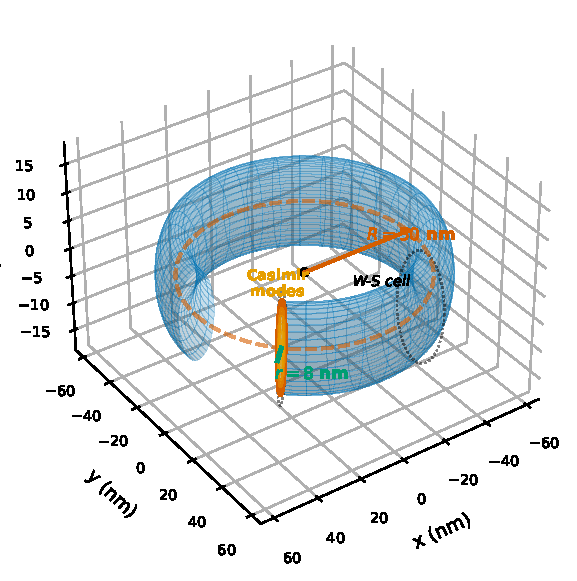
\includegraphics[width=0.7\textwidth]{figures/toroidal_geometry_3d.pdf}
\caption{\textbf{Toroidal hopfion geometry (3D visualization).} Hopfion vortex core has minor radius $r \approx a_H \approx 8$ nm (healing length) and major ring radius $R \approx \xi \approx 50$ nm (coherence length). Aspect ratio $x = 2\pi r/R \approx 1.0$ places the system in the fat-torus regime where the proximity force approximation breaks down and full Bessel mode sum is required, yielding $\mathcal{F}(x) = \Flock$ and $E_{\mathrm{vac}}=\Evac$.}
\label{fig:torus}
\end{figure}

\begin{figure}[htbp]
\centering
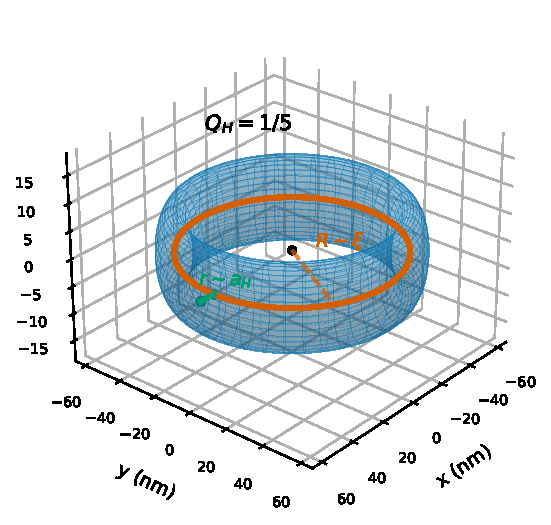
\includegraphics[width=0.6\columnwidth]{figures/hopfion_torus_3d_mpl.pdf}
\caption{\textbf{3D hopfion torus geometry.} The vortex core centerline (red major circle, radius $R \approx \xi \approx 50$ nm) defines the toroidal Casimir cavity. The minor radius $r \approx a_H \approx 8$ nm sets the cavity gap. Purple curves represent Hopf fibration field lines carrying topological charge $Q_H = 1/5$. The aspect ratio $x = 2\pi r/R \approx 1.0$ places the system in the fat-torus regime requiring full Bessel mode sum.}
\label{fig:hopfion_torus_3d}
\end{figure}

The zero-point amplitude $A_{\text{ZPF}}$ in Eq.~\eqref{eq:gap} is not a free parameter; it is fixed by the Casimir energy of the vortex-ring structure of each hopfion in the \TEVC{}. Each hopfion has a vortex core of topological radius $r \sim a_H$ (minor) and a ring radius $R$ (major). The Casimir energy of the resulting toroidal cavity determines the vacuum stress inside the core and, through that, the effective amplitude of the zero-point field felt by the condensate.

\subsection{Toroidal spectral form}

The vacuum energy used throughout is the two-dimensional toroidal spectral form
\begin{equation}
E_{\mathrm{vac}} = \frac{1}{4\pi^2} \cdot \frac{\hbar c_s}{r} \cdot \mathcal{F}(x),
\qquad
\mathcal{F}(x) = \sum_{n=1}^\infty K_0(n x), \quad x = \frac{2\pi r}{R},
\label{eq:modesum}
\end{equation}
with $K_0$ the modified Bessel function of the second kind. For $r = 8$ nm and $R = 50$ nm one has $x = 2\pi r/R = 1.0053$, in the fat-torus regime where a proximity-force plate approximation does not apply. Equation~\eqref{eq:modesum} is a phononic spectral sum on the torus, not a three-dimensional electromagnetic scattering-matrix Casimir energy.

\subsection{Numerical Calculation}

We evaluate Eq.~\eqref{eq:modesum} by summing $K_0(nx)$ (asymptotic expansion for $z>0.5$, Abramowitz--Stegun 9.8.1--9.8.6). For $x = 1.0053$ the sum converges to
\begin{equation}
\mathcal{F}(x = 1.0053) = \Flock.
\end{equation}
With $\hbar c_s = \hbarcs$ this yields
\begin{equation}
\boxed{E_{\mathrm{vac}} = \Evac.}
\end{equation}
The corresponding geometric amplitude is $A_{\mathrm{geom}}=E_{\mathrm{vac}}/(\hbar c_s)=\Ageom$.

\begin{figure}[htbp]
\centering
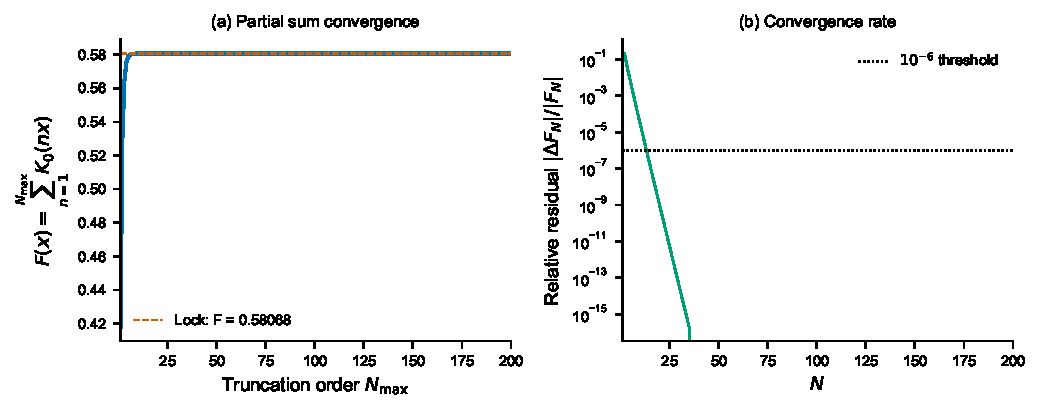
\includegraphics[width=0.8\textwidth]{figures/computed_vacuum_convergence.pdf}
\caption{\textbf{Casimir mode sum convergence.} Partial sum $\mathcal{F}_N(x) = \sum_{n=1}^N K_0(nx)$ as a function of the number of winding modes $N$, for the fat-torus aspect ratio $x = 2\pi r/R = 1.0053$. The sum saturates by $N = 14$ to $\mathcal{F} = \Flock$, demonstrating rapid convergence driven by the exponential decay of $K_0(z)$ at large argument. The final vacuum energy $E_{\mathrm{vac}} = \Evac$ is stable to better than $10^{-6}$ beyond 14 modes.}
\label{fig:vacuum_convergence}
\end{figure}

\begin{figure}[htbp]
\centering
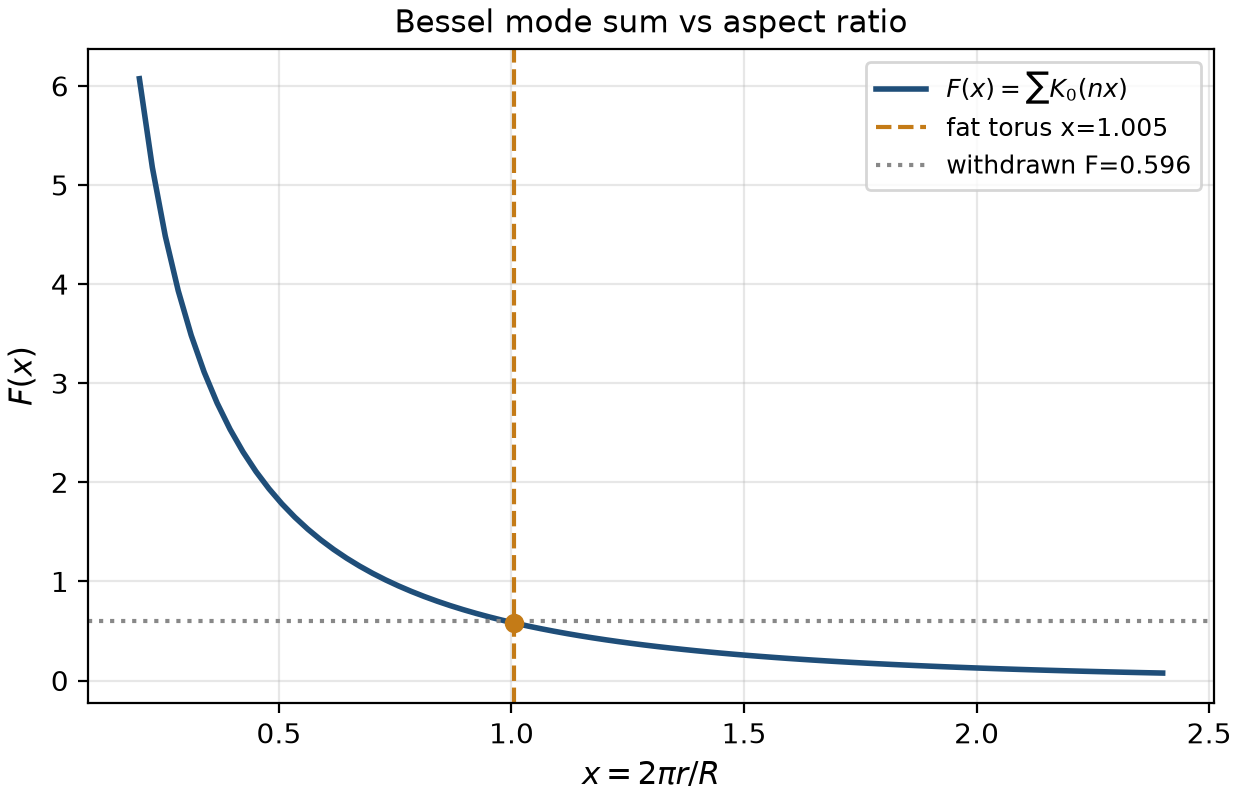
\includegraphics[width=0.7\textwidth]{figures/bridge_F_fat_torus.png}
\caption{\textbf{Spectral form factor $F(x)$ for the fat-torus geometry.} The form factor $F(x) = \sum_{n=1}^\infty K_0(nx)$ evaluated at the locked aspect ratio $x = 2\pi r/R = 1.0053$ (vertical marker). The rapid exponential suppression of $K_0(nx)$ for $n \geq 2$ ensures that only the lowest winding modes contribute appreciably. At the physical aspect ratio, $F = \Flock$, yielding $E_{\mathrm{vac}} = (1/4\pi^2)(\hbar c_s/r)\,F = \Evac$.}
\label{fig:F_fat_torus}
\end{figure}

\subsection{Zero-Point Amplitude}

The geometric amplitude associated with~\eqref{eq:modesum} is
\begin{equation}
A_{\mathrm{geom}} = \frac{E_{\mathrm{vac}}}{\hbar c_s} = \Ageom,
\end{equation}
or $A_{\mathrm{geom}} R \approx 0.0919$ on $R=50$\,nm. This is the amplitude that enters $\alpha=\lambda E_{\mathrm{vac}}/\Delta_0$. Jacobi $\vartheta_3$ is a distinct regularized spectral object and is not identified with $F(x)$.

\subsection{Self-Consistency Loop}

\begin{figure}[htbp]
\centering
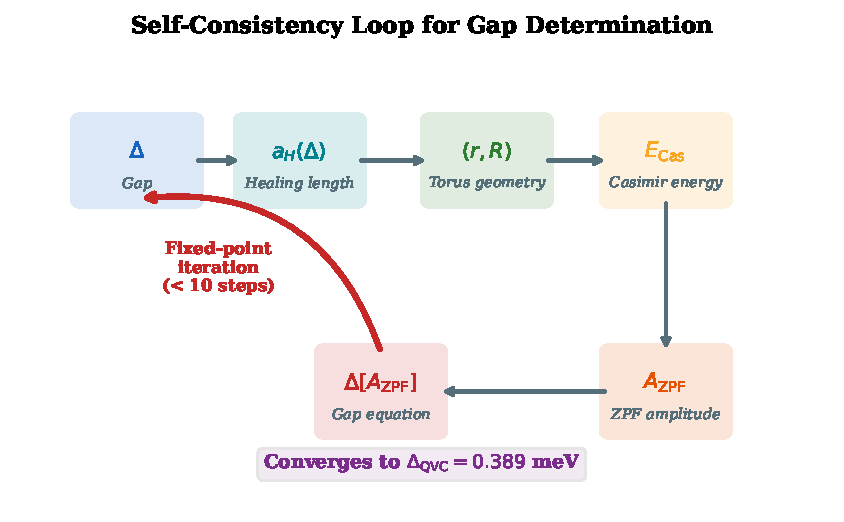
\includegraphics[width=0.65\textwidth]{figures/self_consistency_flowchart.pdf}
\caption{\textbf{Self-consistency on the frozen cavity.} Geometry $(r,R)$ and $a_H=r$ are held fixed. $E_{\mathrm{vac}}$ is the Bessel spectral form. Participation $\lambda$ maps $E_{\mathrm{vac}}$ into $\alpha$; unit $\lambda$ lies beyond the fold ($\alpha/\alpha_c\approx 1.18$). Static physics at the working point uses $\lambda^\star=\lstar$ and $\Delta^\star=\Deltastar$.}
\label{fig:loop}
\end{figure}

The cavity geometry is held at $a_H=r$. There is no running-healing loop $\Delta\to a_H(\Delta)\to E_{\mathrm{vac}}$: $E_{\mathrm{vac}}$ is computed from the frozen torus, and participation $\lambda$ enters only through $\alpha=\lambda E_{\mathrm{vac}}/\Delta_0$ (Section~\ref{sec:bridge}). At $\lambda=1$ the map lies beyond the fold. The working static root is
\begin{equation}
\boxed{\Delta^\star = \Deltastar \quad (\lambda^\star=\lstar),}
\end{equation}
a $\redstar$ reduction from $\Delta_{\text{ex}} = 2J = \Deltaex$, with maximum physical-branch reduction $\redmax$ at $\Delta_c=\Deltac$.



\section{Derived $\alpha$--$E_{\mathrm{vac}}$ Bridge and Participation $\lambda$}
\label{sec:bridge}

The fat-torus freeze $(r,R)=(8,50)$\,nm, the spectral form
\begin{equation}
E_{\mathrm{vac}}=\frac{1}{4\pi^2}\frac{\hbar c_s}{r}\,F\!\left(\frac{2\pi r}{R}\right),\qquad
F(x)=\sum_{n=1}^\infty K_0(nx),
\end{equation}
and package $\hbar c_s=\hbarcs$ fix the vacuum energy independently of a running healing length. Frozen-cavity geometry sets $a_H=r=\mathrm{const}$, so
\begin{equation}
\ell(r)=\ln\frac{\Delta_0 r}{2\hbar c_s}+\gamma_E=\elllock.
\end{equation}
Identifying $A=E_{\mathrm{vac}}/(\hbar c_s)$ and $\alpha=\hbar c_s A/\Delta_0$ yields the boxed bridge
\begin{equation}
\alpha=\lambda\frac{E_{\mathrm{vac}}}{\Delta_0}.
\label{eq:bridge}
\end{equation}
The gap map $\delta=1+\alpha(\ln\delta+\ell)$ has a saddle-node fold at $\alpha_c=\delta_c=\alphac$, hence $\Delta_c=\Deltac$. Unit participation ($\lambda=1$) gives $\alpha/\alpha_c\approx 1.180>1$: there is no physical static $\Delta^*$ at $\lambda=1$. A physical static gap exists for $\lambda\le\lambda_{\mathrm{fold}}=\alpha_c\Delta_0/E_{\mathrm{vac}}=\lfold$. The recommended working point is
\begin{equation}
\lambda^\star=0.90\,\lambda_{\mathrm{fold}}=\lstar,\qquad \Delta^\star=\Deltastar
\end{equation}
($61.3\%$ reduction from $\Delta_0=\Deltaex$). The deepest static reduction on the physical branch is $81.8\%$ at the fold. Running healing $a_H=\hbar c_s/\Delta$ is a distinct theory from the frozen-cavity freeze used here.

Catalyzon hybridization is a parallel channel: $\Delta_{\mathrm{cat}}=\Delta_{\mathrm{ex}}-g_0$ with democratic $\lambda_{\min}=-g_0$ (multiplicity $N-1$). Fold, catalyzon, and truncated GPE dynamics are not additive percentages of a single baseline.

\begin{figure}[htbp]
\centering
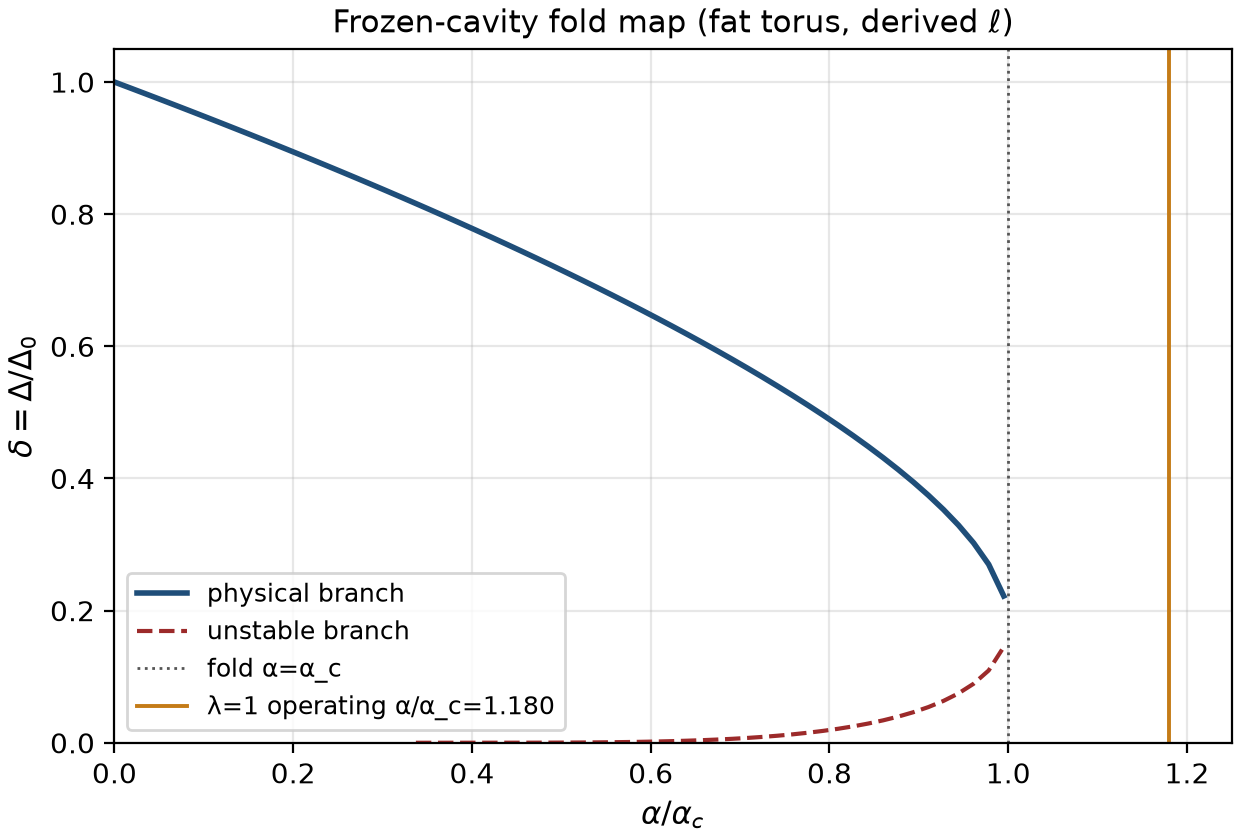
\includegraphics[width=0.7\textwidth]{figures/bridge_fold_operating_point.png}
\caption{\textbf{Bridge fold with operating point.} Gap map physical and unstable branches $\delta_\pm(\alpha/\alpha_c)$ with locked $\ell = \elllock$. Gold square: recommended working point $\lambda^\star = \lstar$ ($\Delta^\star = \Deltastar$, $\alpha^\star/\alpha_c = 0.900$). Red circle: fold critical point ($\alpha_c = \alphac$, $\delta_c = \alphac$). Arrow indicates the direction of increasing vacuum participation $\lambda$. The gap reduction from $\Delta_0$ to $\Delta^\star$ is $\redstar$; maximum physical-branch reduction at the fold is $\redmax$.}
\label{fig:bridge_fold_operating}
\end{figure}

\begin{figure}[htbp]
\centering
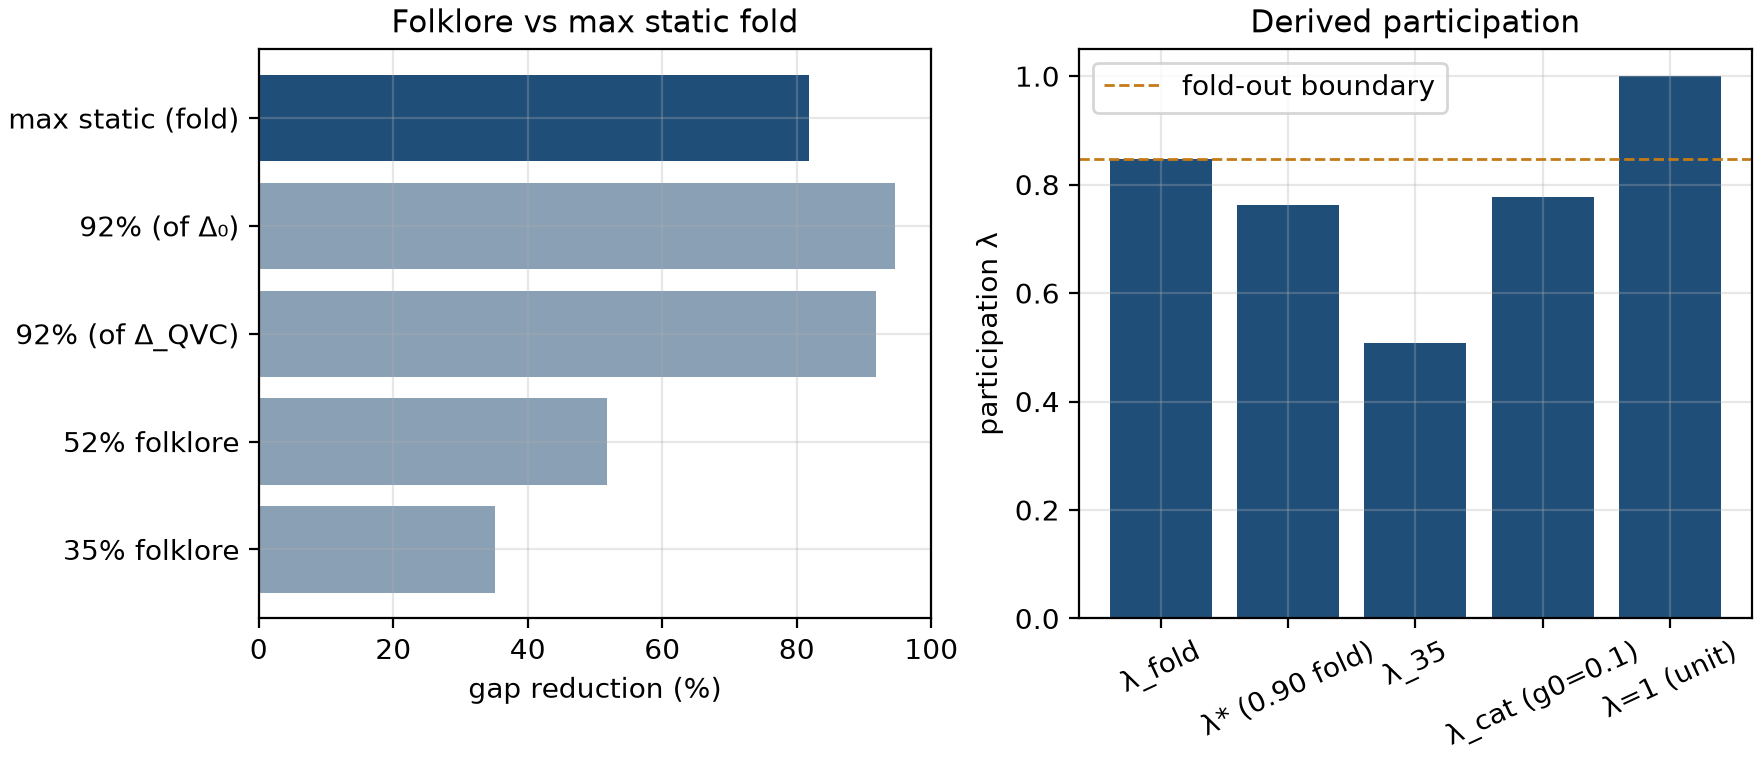
\includegraphics[width=0.65\textwidth]{figures/bridge_gap_reduction_lambda.png}
\caption{\textbf{Gap reduction as a function of participation $\lambda$.} Physical-branch gap $\Delta(\lambda)$ computed from the bridge relation $\alpha = \lambda\,E_{\mathrm{vac}}/\Delta_0$ inserted into the gap map. The gap decreases monotonically with $\lambda$, dropping from $\Delta_0 = \Deltaex$ at $\lambda = 0$ to $\Delta_c = \Deltac$ at $\lambda_{\mathrm{fold}} = \lfold$. Vertical marker at $\lambda^\star = \lstar$ shows the locked working point.}
\label{fig:gap_reduction_lambda}
\end{figure}

\section{Vortex sector, competing infrared scales, and \BKT{} implications}
\label{sec:vortex_rg}

The excitonic order parameter admits a polar decomposition before any renormalization-group analysis,
\begin{equation}
\Psi(\mathbf{r})=\rho(\mathbf{r})\,e^{i\theta(\mathbf{r})}.
\label{eq:polar}
\end{equation}
The locked gap map of Section~\ref{sec:gap} lives in the amplitude $\rho$. The vortex sector of the theory lives in the phase $\theta$. Together the two sectors furnish a competing-scale structure: a saddle-node fold in $\rho$, and a Kosterlitz--Thouless unbinding surface in the stiffness of $\theta$. When a physical drive reaches the KT surface first, the implied gap closing is a Berezinskii--Kosterlitz--Thouless essential singularity. That implication is part of the theory; it is stated as hypothesis H-VRG1 and is evaluated below by the computational suite C1--C6.

Option~A* freezes the toroidal cavity, so the vacuum amplitude---and therefore $\alpha$---does not run with the KT scale $\ell=\ln(L/a_c)$. The suite therefore scans frozen $\alpha$ along the locked physical branch $\delta_+(\alpha)$. Kosterlitz's coupling is $K=\kappa/T_{\mathrm{eff}}$, with critical value $K_c=2/\pi$. No bare transition temperature is inserted by hand, and no chain-rule $\beta_\alpha$ is integrated.

\begin{center}
\fcolorbox{oiBlue}{oiBlue!6}{%
\parbox{0.94\linewidth}{\small
\textbf{Defect vocabulary.}
A \textbf{hopfion} is a map $S^3\to S^2$ with fractional Hopf charge $Q_H=1/N$, realized here as a toroidal Casimir cavity.
A \textbf{2D phase vortex} is a point defect in the moir\'e plane with $\oint\nabla\theta\cdot d\mathbf{l}=2\pi n$; this is the \BKT{} defect of the present section.
A \textbf{Chern--Simons fluxon} is a $2\pi$ winding that binds flux $\Phi_{\mathrm{CS}}=2\pi/N$ at level $k=2N$.
The three objects are distinct.
}}
\end{center}

\subsection{Two-sector decomposition}
\label{sec:two_sector}

Substituting Eq.~\eqref{eq:polar} into the bulk \TQGL{} energy of Section~\ref{sec:tqgl} separates a Higgs potential for $\rho$ from a phase stiffness for $\theta$,
\begin{equation}
\mathcal{F}_{\mathrm{bulk}}[\rho,\theta]
=\int\mathrm{d}^2r\Biggl[
\alpha_{\mathrm{GL}}\rho^2+\frac{\beta}{2}\rho^4
+\kappa_{\mathrm{GL}}\bigl(|\nabla\rho|^2+\rho^2|\nabla\theta|^2\bigr)
\Biggr],
\label{eq:two_sector}
\end{equation}
up to the Chern--Simons, Berry, and Skyrme terms retained in the parent functional. Here $\kappa_{\mathrm{GL}}$ is the Ginzburg--Landau gradient weight written $\kappa$ in Section~\ref{sec:tqgl}, and $\alpha_{\mathrm{GL}}$ is the Landau mass, distinct from the gap-map coupling $\alpha$ of Section~\ref{sec:gap}. Equation~\eqref{eq:two_sector} captures the algebra of the split. The fold of the amplitude map at $\alpha_c=\delta_c=\alphac$, $\Delta_c=\Deltac$ is a locked input. Vortex unbinding is the content of the phase sector.

The live-gap estimator $\Delta_{\mathrm{live}}[\psi]=\Delta_0\sqrt{n_w[\psi]/n_{\mathrm{ref}}}$ of Section~\ref{sec:dynamics} is an amplitude proxy. A field whose modulus remains finite while $\theta$ disorders still returns a nonzero $\Delta_{\mathrm{live}}$. Amplitude and phase diagnostics therefore complement one another: a $1$\,ps trajectory with $\Delta_{\mathrm{live}}(1\,\mathrm{ps})=\Deltaliveone$ constrains $\rho$, while $g(r)$ and the stiffness flow constrain $\theta$.

\begin{figure}[htbp]
\centering
% Two-sector split: amplitude fold vs 2D phase vortex RG
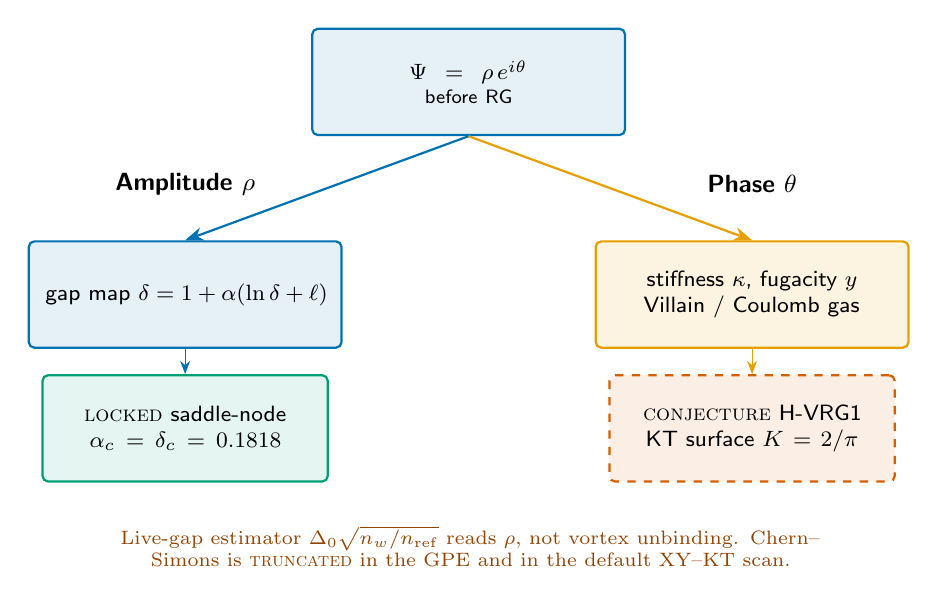
\begin{tikzpicture}[
  font=\sffamily\footnotesize,
  box/.style={draw, rounded corners=2pt, align=center, inner sep=6pt,
    text width=3.55cm, minimum height=1.35cm, line width=0.8pt},
  amp/.style={box, draw=oiBlue, fill=oiBlue!10},
  ph/.style={box, draw=oiOrange, fill=oiOrange!12},
  lock/.style={box, draw=oiGreen, fill=oiGreen!10, text width=3.2cm},
  conj/.style={box, draw=oiVerm, fill=oiVerm!10, dashed, text width=3.2cm},
]
\node[font=\sffamily\small\bfseries] at (0,3.55) {Amplitude $\rho$};
\node[font=\sffamily\small\bfseries] at (7.2,3.55) {Phase $\theta$};
\node[amp] (psi) at (3.6,4.85) {$\Psi=\rho\,e^{i\theta}$\\[-1pt]{\scriptsize before RG}};
\node[amp] (fold) at (0,2.15) {gap map $\delta=1+\alpha(\ln\delta+\ell)$};
\node[lock] (sn) at (0,0.45) {\statuslocked{} saddle-node\\$\alpha_c=\delta_c=\alphac$};
\node[ph] (xy) at (7.2,2.15) {stiffness $\kappa$, fugacity $y$\\Villain / Coulomb gas};
\node[conj] (kt) at (7.2,0.45) {\statusconjecture{} H-VRG1\\KT surface $K=2/\pi$};
\draw[-{Stealth}, oiBlue, thick] (psi.south) -- (fold.north);
\draw[-{Stealth}, oiOrange, thick] (psi.south) -- (xy.north);
\draw[-{Stealth}, oiBlue] (fold.south) -- (sn.north);
\draw[-{Stealth}, oiOrange] (xy.south) -- (kt.north);
\node[font=\scriptsize, text width=10.5cm, align=center, oiVerm!70!black]
  at (3.6,-1.05) {Live-gap estimator $\Delta_0\sqrt{n_w/n_{\mathrm{ref}}}$ reads $\rho$, not vortex unbinding.
  Chern--Simons is \statustruncated{} in the GPE and in the default XY--KT scan.};
\end{tikzpicture}

\caption{\textbf{Two-sector split.} The locked fold is an amplitude phenomenon. Vortex RG is a phase phenomenon. The live-gap estimator reads $\rho$. Chern--Simons is truncated from the default XY--KT scan, matching the GPE truncation of Section~\ref{sec:dynamics}.}
\label{fig:two_sector}
\end{figure}

\subsection{C1: phase stiffness}
\label{sec:stiffness}

The 2D phase stiffness (superfluid density) extracted from Eq.~\eqref{eq:two_sector} is not $\kappa_{\mathrm{GL}}$ itself. Matching $\kappa_{\mathrm{GL}}|\nabla\Psi|^2$ to the conventional $(\rho_s/2)|\nabla\theta|^2$ with $\Psi=\sqrt{n_0}\,\rho\,e^{i\theta}$ gives
\begin{equation}
\kappa\equiv\rho_s=2 n_0\kappa_{\mathrm{GL}}\langle\rho^2\rangle+\kappa_{\mathrm{geom}},
\label{eq:kappa}
\end{equation}
where $\kappa_{\mathrm{GL}}=\Delta_0 a_H^2$ follows from the truncated GPE kinetic match and $\langle\rho^2\rangle=\delta_+(\alpha)^2$ is read from the locked physical branch through the live-gap identification. The density unit is the healing-disk ansatz $n_0=1/(\pi a_H^2)$, which converts dimensionless $|\psi|^2\sim 1$ into a 2D density and makes the conventional piece at unit amplitude equal to $2\Delta_0/\pi$, independent of $a_H$. The geometric weight $\kappa_{\mathrm{geom}}$ is a frozen Peotta--T\"orm\"a floor~\cite{PeottaTorma2015},
\begin{equation}
\kappa_{\mathrm{geom}}=\frac{\Delta_0}{2\pi},
\label{eq:kappa_geom}
\end{equation}
treated as an ansatz: it is not a Brillouin-zone integral of the TEVC quantum metric, and it need not vanish with $\delta$. From here on in this section, $\kappa$ means the stiffness~\eqref{eq:kappa}. A uniform phase-twist check on the same conventional piece agrees with $2 n_0\kappa_{\mathrm{GL}}\langle\rho^2\rangle$ to machine precision.

On this primary vortex-RG closure---healing-disk $n_0$ plus the frozen geometric floor~\eqref{eq:kappa_geom}---one finds $\kappa_{\mathrm{UV}}\approx\kappauvfloor$ at $\alpha=0$ and $\kappa(\alpha_c)\approx 0.108$\,meV at the fold. With $T_{\mathrm{eff}}=T^*=\Tstar$ the Kosterlitz couplings are $K(\alpha=0,T^*)\approx\Kuvfloor$ and $K(\alpha_c,T^*)\approx\Kfoldfloor$, both far above $K_c=2/\pi\approx 0.637$. A Qi--Wu--Zhang toy metric (Section~\ref{sec:c1_trackb}) is a second labeled C1 estimator ($\kappa_{\mathrm{UV}}^{\mathrm{toy}}=\kappauvtoy$, $K_{\mathrm{fold}}(T^*)=\KfoldTstar$); both miss KT at $T^*$ before the fold. A conventional-only variant with $\kappa_{\mathrm{geom}}=0$ is retained as a labeled alternative; its ultraviolet stiffness is $2\Delta_0/\pi\approx 0.382$\,meV. The energy of an isolated 2D phase vortex in a system of size $L$ with core cutoff $a_c$ is
\begin{equation}
E_v=\pi\kappa\ln(L/a_c)+E_{\mathrm{core}}.
\label{eq:Ev}
\end{equation}
The gap $\Delta$ sets a scale for $\rho$ and for $a_c\sim\hbar c_s/\Delta$. \BKT{} physics is a statement about whether $\kappa/T_{\mathrm{eff}}$ flows through the universal jump
\begin{equation}
\kappa(T_{\mathrm{BKT}}^-)=\frac{2T_{\mathrm{BKT}}}{\pi}.
\label{eq:universal_jump}
\end{equation}
A finite $\Delta_c$ at the fold is compatible with a still-superfluid phase, with a plasma of 2D phase vortices, or with a rounded quantum crossover; the amplitude map and the stiffness flow decide jointly.

\subsection{Coulomb gas and Villain action}
\label{sec:villain}

The effective theory for 2D phase vortices is the XY/Villain model~\cite{Kosterlitz1973,Villain1975,Jose1977}, equivalently the integer Coulomb gas
\begin{equation}
\frac{H}{T_{\mathrm{eff}}}
=2\pi K\sum_{i<j}n_i n_j\ln\frac{|r_i-r_j|}{a_c}
+\frac{E_{\mathrm{core}}}{T_{\mathrm{eff}}}\sum_i n_i^2,
\label{eq:villain}
\end{equation}
with spin-wave piece $S_{\mathrm{sw}}[\theta]=\frac{K}{2}\int(\nabla\theta)^2$. We adopt the Kosterlitz normalization $K=\kappa/T_{\mathrm{eff}}$ (not the Jos\'e--Kadanoff $\tilde K=\pi\kappa/T_{\mathrm{eff}}$), so that the one-loop flow
\begin{equation}
\frac{\mathrm{d}K^{-1}}{\mathrm{d}\ell}=4\pi^3 y^2,\qquad
\frac{\mathrm{d}y}{\mathrm{d}\ell}=(2-\pi K)y
\label{eq:kt_flow}
\end{equation}
has critical point $K_c=2/\pi$. Equivalently, $\pi\kappa/T_{\mathrm{eff}}=\pi K$ equals $2$ on the universal jump~\eqref{eq:universal_jump}. Equation~\eqref{eq:kt_flow} is the vortex-RG sector of the theory. Its derivation from the microscopic \TQGL{} functional proceeds through a Villain reduction, which we state as an ansatz: the phase sector is governed by~\eqref{eq:villain}--\eqref{eq:kt_flow} once amplitude fluctuations have been integrated at the scale $a_c$. The flow equations are derived as an effective theory; the Villain reduction from the full \TQGL{} functional is treated as an ansatz. The fugacity is the textbook form $y=\exp(-E_{\mathrm{core}}/T_{\mathrm{eff}})$.

\subsection{C2: winding-one core}
\label{sec:c2_core}

The defect that enters~\eqref{eq:Ev} is a winding-$1$ radial Gross--Pitaevskii vortex in the moir\'e plane, not a hopfion and not a Chern--Simons fluxon. Integrating the truncated GP energy on a disk and subtracting the infrared logarithm at the healing-length cutoff $a_c=\xi=8$\,nm yields $E_{\mathrm{core}}/\kappa\approx 0.343$, with the cutoff itself an ansatz. That ratio sets the bare fugacity along the branch, $y=\exp\bigl[-(E_{\mathrm{core}}/\kappa)K\bigr]$. Because $E_{\mathrm{core}}/\kappa$ is $\mathcal{O}(1)$ rather than $\mathcal{O}(10)$, finite $y$ can matter even when the bare coupling still lies well above $2/\pi$: the infrared plasma is a separatrix phenomenon, not merely a $K<K_c$ crossing of the ultraviolet data.

\subsection{Competing infrared scales}
\label{sec:competing}

Two surfaces compete in the $(\alpha,K,y)$ space of a driven TEVC.

\begin{theorem}[Competing-scale criterion]
\label{thm:competing}
On the locked amplitude theory the fold surface is
\begin{equation}
\alpha=\alpha_c,\qquad \Delta=\Delta_c>0.
\label{eq:fold_surface}
\end{equation}
On the Villain target~\eqref{eq:kt_flow} the KT surface is
\begin{equation}
K=2/\pi,\qquad y\to 0,
\label{eq:kt_surface}
\end{equation}
with $\Delta\to 0$ only if $\Delta$ tracks a positive power of $\kappa$ after unbinding. Hypothesis H-VRG1 holds if and only if the physical drive path hits the KT surface \emph{before} the fold. If $\kappa(A)$ remains larger than $\kappa_{\mathrm{BKT}}$ at $\alpha=\alpha_c$ and finite-$y$ flow stays bound, the fold wins and the gap map retains a finite $\Delta_c$.
\end{theorem}

Whether a given protocol satisfies it is a property of $\kappa(\alpha)$, $E_{\mathrm{core}}/\kappa$, and $T_{\mathrm{eff}}$.

\begin{hypothesis}[H-VRG1]
Including a 2D phase-vortex fugacity in the RG of $\theta=\arg\Psi$ converts the locked saddle-node fold into a \textup{\BKT{}} essential singularity $\Delta\sim\exp(-C/\sqrt{A_c-A})$ with continuous gap vanishing, whenever the drive path of Theorem~\ref{thm:competing} reaches the KT surface first.
\end{hypothesis}

H-VRG1 is a conjecture. The C1 stiffness is a computed closure with ansatz inputs, not a Brillouin-zone theorem, so the competing-scale diagram below is the implication of that closure.

\subsection{Chern--Simons statistics: truncation or anyon plasma}
\label{sec:anyon}

The parent functional contains a Chern--Simons term at level $k=2N$, which attaches flux $\Phi_{\mathrm{CS}}=2\pi/N$ to a $2\pi$ winding. Ordinary XY--KT assumes bosonic integer 2D phase vortices. An anyonic plasma changes the Coulomb coupling.

Two consistent options exist. The first, adopted for the default scan and matching the GPE of Section~\ref{sec:dynamics}, is to \emph{truncate} Chern--Simons, Berry, and Skyrme from the vortex sector: the flow~\eqref{eq:kt_flow} then applies to ordinary 2D phase vortices, and CS fluxons are outside the calculation. The second is to restore level $k=2N$ and treat 2D phase vortices as anyons with statistical angle
\begin{equation}
\theta_{\mathrm{stat}}=\frac{\pi}{N}\qquad(N=5\Rightarrow \theta_{\mathrm{stat}}=\pi/5).
\label{eq:theta_stat}
\end{equation}
A Wen--Zee-inspired shift of the KT criterion~\cite{WenZee1992,Wen1995} then reads
\begin{equation}
K_c^{\mathrm{anyon}}=\frac{2}{\pi}\Bigl(1-\frac{\theta_{\mathrm{stat}}}{\pi}\Bigr)^2
=\frac{2}{\pi}\Bigl(1-\frac{1}{N}\Bigr)^2,
\label{eq:Kc_anyon}
\end{equation}
which for $N=5$ lowers $K_c$ from $2/\pi\approx 0.637$ to $\approx 0.407$. A lower $K_c$ moves the KT surface toward weaker stiffness. Equation~\eqref{eq:Kc_anyon} remains conjectural unless the anyon-Coulomb-gas algebra is derived from the \TQGL{} Chern--Simons term; it is displayed so that the truncation is explicit, and it is never mixed into the truncated default.

\subsection{C3: competing-scale scan}
\label{sec:vrg_python}

On the primary closure---healing-disk $n_0$ plus the frozen geometric floor---at $T^*=\Tstar$, Kosterlitz flow at frozen $\alpha$ remains bound all the way to the fold. The infrared coupling at $\alpha_c$ is $K(\alpha_c)\approx 10.57\gg 2/\pi$: the fold is reached first. Restoring the labeled anyon threshold~\eqref{eq:Kc_anyon} does not change the winner on this $\kappa(\alpha)$. The same $E_{\mathrm{core}}/\kappa\approx 0.34$ that would be dangerous near $K\sim 1$ is harmless at $K\sim 10$, because $y=\exp(-0.34 K)$ is then exponentially small.

The conventional-only variant ($\kappa_{\mathrm{geom}}=0$) at the same $T^*$ is different. Bare $K$ still stays above $2/\pi$ through $\alpha_c$, so there is no ultraviolet $K<K_c$ crossing. Finite-$y$ flow, however, hits the plasma separatrix at $\alpha/\alpha_c\approx 0.945$: KT before the fold, as an infrared phenomenon. The computed core ratio is large enough for that separatrix even though the geometric floor is what had kept the primary branch bound.

Raising $T_{\mathrm{eff}}$ opens a temperature window for the vortex sector even on the primary closure. Below $\sim 50$\,mK both closures remain bound out to $\alpha_c$. At $T^*$ only conventional-only unbinds. At $T_{\mathrm{eff}}=0.5$\,K the primary branch already plasmas at $\alpha/\alpha_c\approx 0.819$; at $1$\,K the plasma station has moved in to $\alpha/\alpha_c\approx 0.302$. That window is the physically interesting content of the sector: whether a laboratory protocol sits on the fold side or the KT side of Theorem~\ref{thm:competing} is a joint question of stiffness closure and temperature, not an algebraic identity.

\begin{figure}[htbp]
\centering
% Textbook KT flow at frozen α: primary bound vs conv-only plasma (C3)
\begin{tikzpicture}
\begin{axis}[
  width=0.92\linewidth,
  height=6.4cm,
  xmode=log,
  ymode=log,
  xlabel={$K=\kappa/T_{\mathrm{eff}}$},
  ylabel={fugacity $y$},
  xmin=0.2, xmax=60,
  ymin=1e-6, ymax=2,
  legend style={draw=none, at={(0.98,0.98)}, anchor=north east, font=\small, cells={anchor=west}},
  tick label style={font=\small},
  label style={font=\small},
  clip=true,
]
\addplot[oiGreen, line width=1.5pt, mark=*, mark size=1.5pt]
  table[x index=1, y index=2, skip first n=1] {data/vortex_rg_flow_uv.dat};
\addlegendentry{primary UV (bound)}
\addplot[oiBlue, line width=1.5pt, mark=*, mark size=1.5pt]
  table[x index=1, y index=2, skip first n=1] {data/vortex_rg_flow_star.dat};
\addlegendentry{primary $\lambda^\star$ (bound)}
\addplot[oiSky, line width=1.5pt, dashed, mark=*, mark size=1.5pt, every mark/.append style={solid}]
  table[x index=1, y index=2, skip first n=1] {data/vortex_rg_flow_nearfold.dat};
\addlegendentry{primary near fold (bound)}
\addplot[oiVerm, line width=1.5pt]
  table[x index=1, y index=2, skip first n=1] {data/vortex_rg_flow_conv_plasma.dat};
\addlegendentry{conv-only IR plasma}
\draw[black!50, densely dotted, line width=0.8pt]
  (axis cs:0.63662,1e-6) -- (axis cs:0.63662,2);
\node[font=\small, oiBlue, anchor=south, rotate=90] at (axis cs:0.85,3e-4) {$K_c=2/\pi$};
\end{axis}
\end{tikzpicture}

\caption{\textbf{Kosterlitz flow at frozen $\alpha$ and $T^*$.} Primary-closure trajectories at $\alpha/\alpha_c=0.30$, at $\lambda^\star$, and near the fold all run to $y\to 0$ with $K\gg 2/\pi$ (bound). A conventional-only station at the finite-$y$ onset $\alpha/\alpha_c\approx 0.945$ runs to a plasma. Option~A* holds $\alpha$ fixed; there is no $\beta_\alpha$.}
\label{fig:vrg_flow}
\end{figure}

\begin{figure}[htbp]
\centering
% Competing IR scales along the locked physical branch (C1/C3 at T*)
\begin{tikzpicture}
\begin{axis}[
  width=0.92\linewidth,
  height=6.4cm,
  ymode=log,
  xlabel={$\alpha/\alpha_c$},
  ylabel={$K=\kappa/T^*$},
  xmin=0, xmax=1.02,
  ymin=0.3, ymax=70,
  legend style={draw=none, fill=white, fill opacity=0.85, at={(0.02,0.02)}, anchor=south west, font=\small, cells={anchor=west}},
  tick label style={font=\small},
  label style={font=\small},
  grid=both,
  major grid style={line width=0.3pt, draw=black!20},
  minor grid style={line width=0.15pt, draw=black!8},
  minor x tick num=4,
]
\addplot[oiBlue, line width=1.5pt]
  table[x index=0, y index=1, skip first n=1] {data/competing_scales.dat};
\addlegendentry{primary $K$ (C1)}
\addplot[oiOrange, line width=1.5pt, dashed]
  table[x index=0, y index=2, skip first n=1] {data/competing_scales.dat};
\addlegendentry{conventional-only}
\addplot[oiVerm, densely dashed, line width=0.8pt]
  coordinates {(0,0.63662) (1.02,0.63662)};
\addlegendentry{$K_c=2/\pi$ (bosonic)}
\addplot[oiPurple, densely dotted, line width=0.8pt]
  coordinates {(0,0.4074) (1.02,0.4074)};
\addlegendentry{$K_c^{\mathrm{anyon}}$ (labeled)}
\addplot[oiGreen, densely dashed, line width=0.8pt]
  coordinates {(0.90,0.3) (0.90,70)};
\addlegendentry{$\lambda^\star$ ($\alpha/\alpha_c=0.90$)}
\node[font=\small, oiGreen, anchor=south west, rotate=90] at (axis cs:0.91,1.0)
  {$\alpha/\alpha_c=0.90$};
\addplot[only marks, mark=*, mark size=2.4pt, oiOrange]
  coordinates {(0.945, 4.04)};
\addlegendentry{conv.\ IR plasma $\approx 0.945\,\alpha_c$}
\end{axis}
\end{tikzpicture}

\caption{\textbf{Competing-scale diagram at $T^*$.} Kosterlitz $K=\kappa/T^*$ along the locked physical branch for the primary C1 closure and the conventional-only variant. The bosonic line $K=2/\pi$ and the labeled anyon line lie far below the primary curve; the fold is reached first. Conventional-only unbinding is a finite-$y$ infrared plasma at $\alpha/\alpha_c\approx 0.945$, marked, not a bare $K<2/\pi$ crossing.}
\label{fig:competing_scales}
\end{figure}

\begin{figure}[htbp]
\centering
% Temperature window: first plasma station vs T_eff (C3)
\begin{tikzpicture}
\begin{axis}[
  width=0.92\linewidth,
  height=5.8cm,
  xmode=log,
  xlabel={$T_{\mathrm{eff}}$ (K)},
  ylabel={first plasma $\alpha/\alpha_c$},
  xmin=0.015, xmax=1.4,
  ymin=0, ymax=1.08,
  legend style={draw=none, at={(0.02,0.12)}, anchor=south west, font=\footnotesize, cells={anchor=west}},
  tick label style={font=\small},
  label style={font=\small},
]
\addplot[oiBlue, thick, mark=*, mark size=2.2pt]
  table[x index=0, y index=2, skip first n=1] {data/Teff_scan.dat};
\addlegendentry{primary (fold $=1$)}
\addplot[oiOrange, thick, dashed, mark=square*, mark size=2.2pt]
  table[x index=0, y index=4, skip first n=1] {data/Teff_scan.dat};
\addlegendentry{conventional-only}
\addplot[oiGreen, densely dashed]
  coordinates {(0.1187,0) (0.1187,1.08)};
\addlegendentry{$T^*=118.7$\,mK}
\addplot[oiVerm, densely dotted]
  coordinates {(0.015,1) (1.4,1)};
\end{axis}
\end{tikzpicture}

\caption{\textbf{Temperature window of the vortex sector.} First $\alpha/\alpha_c$ at which frozen-$\alpha$ flow reaches an infrared plasma, or $\alpha/\alpha_c=1$ if the fold is reached first. The Schwinger crossover $T^*$ is marked. Raising $T_{\mathrm{eff}}$ to $0.5$--$1$\,K lets even the primary closure unbind by finite $y$.}
\label{fig:teff_window}
\end{figure}

\subsection{C4: vacuum driving and the essential-singularity implication}
\label{sec:unbinding_mech}

On the primary $T^*$ scan the flow stays bound, so the locked finite $\Delta_c$ stands: there is no vortex-driven continuous $\Delta\to 0$ on that closure. When a protocol does pass Theorem~\ref{thm:competing}---as the conventional-only variant does at $T^*$---increasing the vacuum amplitude $A$ (equivalently $\alpha$) walks the system along $\delta_+(\alpha)\searrow\delta_c$ while $\kappa$ and $E_{\mathrm{core}}$ fall and $y$ rises. Unbinding occurs if the finite-$y$ separatrix, or $K=2/\pi$, is reached while $\alpha$ is still less than $\alpha_c$. Identifying the KT correlation length with a gap,
\begin{equation}
\Delta\sim\hbar c_s/\xi_{\mathrm{KT}},
\label{eq:delta_xi}
\end{equation}
then produces the essential singularity
\begin{equation}
\Delta(A)\sim\exp\bigl(-C/\sqrt{A_c-A}\bigr)
\label{eq:v9}
\end{equation}
whenever $\Delta$ tracks $\sqrt{\kappa}$ or an equivalent stiffness collapse. Equation~\eqref{eq:delta_xi} is a conjectural identification; Eq.~\eqref{eq:v9} is the \BKT{} implication of the vortex sector (H-VRG1). It is a physical prediction for a protocol that passes Theorem~\ref{thm:competing}, not a replacement of the locked amplitude fold.

\subsection{Finite-size phase correlations}
\label{sec:gr}

Define the 2D phase correlator
\begin{equation}
g(r)=\bigl\langle e^{i[\theta(\mathbf{r})-\theta(0)]}\bigr\rangle.
\label{eq:gr}
\end{equation}
In a Villain spin-wave treatment (vortices omitted) $g(r)\sim r^{-\eta}$ with $\eta=1/(2\pi K)$; at $K=2/\pi$ one has $\eta=1/4$. In a plasma, $g(r)$ is exponential. An effective exponent on a torus of size $L$,
\begin{equation}
\eta_{\mathrm{eff}}(L)=-\frac{\ln g(L/2)}{\ln(L/(2a))},
\label{eq:eta_eff}
\end{equation}
approaches $1/4$ at a putative KT point and rises when vortices proliferate. On the primary $T^*$ branch, $K\sim 10$--$47$ implies a spin-wave $\eta$ of order $10^{-3}$--$10^{-2}$, far below $1/4$, consistent with a still-bound phase. Figure~\ref{fig:gr} shows that family together with the algebraic KT target and an exponential plasma toy; Fig.~\ref{fig:eta_eff} shows $\eta_{\mathrm{eff}}$ along the physical branch. A modest $L=16$ Metropolis XY run remains a program item for sampling vortices rather than spin waves. 
\begin{figure}[htbp]
\centering
% Villain spin-wave g(r) at primary λ* stiffness (C3/C1)
\begin{tikzpicture}
\begin{axis}[
  name=gplot,
  width=0.92\linewidth,
  height=5.6cm,
  xmode=log,
  ymode=log,
  xlabel={$r/a$},
  ylabel={$g(r)$},
  xmin=1, xmax=64,
  ymin=1e-3, ymax=1.2,
  legend style={draw=none, at={(0.02,0.02)}, anchor=south west, font=\footnotesize, cells={anchor=west}},
  tick label style={font=\small},
  label style={font=\small},
]
\addplot[oiBlue, thick]
  table[x index=0, y index=1, skip first n=1] {data/g_r_scaling.dat};
\addlegendentry{spin-wave at $\lambda^\star$}
\addplot[oiOrange, thick, dashed]
  table[x index=0, y index=2, skip first n=1] {data/g_r_scaling.dat};
\addlegendentry{$\eta=1/4$ (KT target)}
\addplot[oiVerm, densely dotted]
  table[x index=0, y index=3, skip first n=1] {data/g_r_scaling.dat};
\addlegendentry{plasma toy}
\end{axis}
\end{tikzpicture}

\caption{\textbf{Phase correlator $g(r)$.} Villain spin-wave decay at the primary $\lambda^\star$ stiffness, the algebraic KT target $\eta=1/4$, and an exponential plasma toy. Vortices are not sampled in the spin-wave curves.}
\label{fig:gr}
\end{figure}

\begin{figure}[htbp]
\centering
% Spin-wave η along the primary T* branch
\begin{tikzpicture}
\begin{axis}[
  width=0.92\linewidth,
  height=6.0cm,
  xlabel={$\alpha/\alpha_c$},
  ylabel={$\eta=1/(2\pi K)$},
  xmin=0, xmax=1.0,
  ymin=0, ymax=0.020,
  legend style={draw=none, at={(0.02,0.98)}, anchor=north west, font=\small, cells={anchor=west}},
  tick label style={font=\small},
  label style={font=\small},
]
\addplot[oiBlue, line width=1.5pt]
  table[x index=0, y index=2, skip first n=1] {data/eta_eff.dat};
\addlegendentry{primary spin-wave $\eta$}
% η_c = 1/4 = 0.25 is far above this range; annotate with upward arrow
\draw[oiVerm, densely dashed, line width=0.8pt, -{Stealth[length=4pt]}]
  (axis cs:0.55,0.016) -- (axis cs:0.55,0.0198);
\node[font=\small, oiVerm, anchor=west] at (axis cs:0.57,0.0175)
  {$\eta_c = \tfrac{1}{4}$ (far above)};
\end{axis}
\end{tikzpicture}

\caption{\textbf{Spin-wave $\eta=1/(2\pi K(\alpha))$ along the primary $T^*$ branch.} With $K(\alpha_c)\approx 10.57$ the exponent remains far below the KT target $\eta=1/4$. The line $\eta=1/4$ is the would-be unbinding marker.}
\label{fig:eta_eff}
\end{figure}

\subsection{C5: fold versus essential singularity}
\label{sec:c5}

On the locked physical branch, $\delta-\delta_c\sim\sqrt{t_A}$ with $t_A=(\alpha_c-\alpha)/\alpha_c$ is a theorem of the amplitude map. A Gaussian comparison of $\tfrac12\ln t_A$ against $1/\sqrt{t_A}$ on $\ln(\delta-\delta_c)$ over $\gtrsim 1.5$ decades in $t_A$ returns a free slope $0.542$ (versus the theorem value $1/2$) and prefers the square root by $\Delta\ell\ell\approx +431$. That comparison is a consistency check on fold data. Vortex-implied $\Delta$ from Eq.~\eqref{eq:delta_xi} is not available on the primary $T^*$ scan, which never unbinds, so the essential-singularity curve in Fig.~\ref{fig:delta_tA} is the H-VRG1 target overlaid on a map that does not contain vortices. The preference for $\sqrt{t_A}$ confirms the locked fold; it is not a statement that a KT surface cannot be hit on a different closure or at a higher $T_{\mathrm{eff}}$.

\begin{figure}[htbp]
\centering
% Fold √ scaling vs H-VRG1 essential singularity (C5)
\begin{tikzpicture}
\begin{axis}[
  width=0.92\linewidth,
  height=6.2cm,
  xmode=log,
  ymode=log,
  xlabel={$t_A=(\alpha_c-\alpha)/\alpha_c$},
  ylabel={$\delta$},
  xmin=1e-3, xmax=1,
  ymin=1e-5, ymax=1.2,
  legend style={draw=none, fill=white, fill opacity=0.85, at={(0.98,0.98)}, anchor=north east, font=\small, cells={anchor=west}},
  tick label style={font=\small},
  label style={font=\small},
]
\addplot[oiBlue, line width=1.5pt]
  table[x index=0, y index=1, skip first n=1] {data/delta_vs_tA.dat};
\addlegendentry{physical branch (\statuslocked)}
\addplot[oiGreen, densely dashed, line width=1.5pt]
  table[x index=0, y index=2, skip first n=1] {data/delta_vs_tA.dat};
\addlegendentry{$\delta_c+B\sqrt{t_A}$}
\addplot[oiVerm, densely dotted, line width=1.5pt]
  table[x index=0, y index=3, skip first n=1] {data/delta_vs_tA.dat};
\addlegendentry{H-VRG1 $e^{-C/\sqrt{t_A}}$}
\addplot[oiOrange, densely dotted, line width=0.8pt]
  coordinates {(1e-3,0.1818) (1,0.1818)};
\end{axis}
\end{tikzpicture}

\caption{\textbf{Amplitude-map scaling on the locked branch.} Physical $\delta(t_A)$ follows $\delta_c+B\sqrt{t_A}$. The dotted essential singularity is the H-VRG1 target of the vortex sector; vortex-implied $\Delta$ is not constructed on the primary $T^*$ scan.}
\label{fig:delta_tA}
\end{figure}

\subsection{C6: thermal versus quantum unbinding}
\label{sec:thermal_quantum}

Classical KT flow requires $T>0$. The TEVC condensation window is $\lesssim 1$\,K; the Schwinger crossover is $T^*=\Tstar$; the live GPE of Section~\ref{sec:dynamics} is $T=0$. At strictly zero temperature the thermal fugacity $y=e^{-E_{\mathrm{core}}/T}$ vanishes and textbook KT does not run. Quantum phase slips, the 2D Bose--Hubbard/Villain dual~\cite{FisherWeichman1989}, or dissipative Ambegaokar--Halperin--Nelson--Siggia (AHNS) dynamics~\cite{Ambegaokar1980,HalperinNelson1978} are then the relevant mechanisms.

\begin{hypothesis}[H-VRG2]
Phonon drag in a Gao--Khalaf-type moir\'e electron--phonon bath places 2D phase vortices in an overdamped regime $\hbar/\tau_v\gtrsim\pi\kappa$, converting a universal jump into a rounded crossover rather than a textbook thermal KT transition.
\end{hypothesis}

Two labeled mobility estimates are compared with the primary $\kappa(\alpha)$ at $T^*$. The phonon amplitude already present in the truncated GPE is $\hbar/\tau_v\sim g_{\mathrm{ph}}=0.1\Delta_0$. An Eliashberg-type OOM with $\lambda_{\mathrm{ep}}=1$ is $\hbar/\tau_v\sim 2\pi\lambda_{\mathrm{ep}}k_BT$. Along the primary branch both give $(\hbar/\tau_v)/(\pi\kappa)\sim 0.04$--$0.19<1$: the vortices are underdamped. A sharp stiffness jump could therefore survive if a KT surface were hit. H-VRG2 is not forced by these estimates; it remains a conjecture pending a microscopically computed vortex mobility.

\subsection{Observables, acceptance, and closures}
\label{sec:vrg_obs}

\begin{table}[htbp]
\centering
\caption{Fold versus vortex-RG observables, as tested by suite C1--C6. Acceptance of H-VRG1 on a given protocol requires the essential-singularity comparison on vortex-inclusive data over $\gtrsim 1.5$ decades in $t_A=(A_c-A)/A_c$, together with $\eta\to 1/4$ in $g(r)$.}
\label{tab:vrg_obs}
\small
\begin{tabular}{@{}llll@{}}
\toprule
Observable & Fold (established) & Vortex RG (conjectured) & Present suite \\
\midrule
$\Delta(A)$ & ends at $\Delta_c$; $\sqrt{t_A}$ & $\Delta\to 0$; $e^{-C/\sqrt{t_A}}$ & C4 bound at $T^*$; C5 on fold data \\
$\kappa$ & need not jump & universal jump~\eqref{eq:universal_jump} & C1 two-sector $\kappa(\alpha)$ \\
$g(r)$ & amplitude death first & algebraic $\to$ exponential & spin-wave at primary $K$ \\
vortex density & not required & proliferates above $A_c$ & C2 core; C3 plasma flag \\
mobility & --- & jump vs AHNS crossover & C6 underdamped at $T^*$ \\
specific heat & mean-field anomaly possible & no latent heat & program \\
\bottomrule
\end{tabular}
\end{table}

The vortex-RG sector is closed by the following statements. The Villain reduction from the \TQGL{} functional is an ansatz. The C1 identity~\eqref{eq:kappa} is derived given the healing-disk $n_0$ and the frozen geometric floor, both of which are ansatzes. Hypothesis H-VRG1 is a conjecture: if the drive path satisfies Theorem~\ref{thm:competing}, the gap closing takes the essential-singularity form~\eqref{eq:v9}. On the primary closure at $T^*$ the fold is reached first; conventional-only stiffness, and the primary closure at $T_{\mathrm{eff}}\sim 0.5$--$1$\,K, populate the KT side of the diagram as finite-$y$ plasmas. Chern--Simons remains truncated from the default scan unless Eq.~\eqref{eq:Kc_anyon} is restored as a labeled option. The locked amplitude fold is the mean-field backbone of the static theory and is independent of whether a given protocol realizes H-VRG1.


\section{Phononic Band Structure and Resonance Condition}
\label{sec:phonons}

\subsection{Moiré Phonon Dispersion}

For \MATBG, the moiré superlattice with period $\lambda_M \approx 13$ nm creates a reduced Brillouin zone with wavevector $K_M = 4\pi/(3\lambda_M) \approx 0.32$ nm$^{-1}$. Phonon dispersion includes contributions from in-plane acoustic phonons (longitudinal $\omega_{\text{LA}}(q) = c_{\text{LA}} q$, transverse $\omega_{\text{TA}}(q) = c_{\text{TA}} q$), out-of-plane flexural modes ($\omega_{\text{ZA}}(q) = \alpha_{\text{ZA}} q^2$), and interlayer shear modes ($\omega_S \sim 10$–30 cm$^{-1}$). Moiré folding creates replicas at $q \pm n K_M$, and interlayer coupling produces flat phonon bands near the Brillouin zone boundaries through hybridization.

\subsection{Resonance Condition}

The resonance condition $\omega_0 = 2\Delta/\hbar$ emerges rigorously from analytic continuation of the retarded self-energy. The one-loop Matsubara self-energy is
\begin{equation}
\Sigma(i\omega_n) = g^2 \int \frac{\mathrm{d}^2 q}{(2\pi)^2} \, T \sum_m D(\mathbf{q}, i\omega_m) G_0(\mathbf{k}-\mathbf{q}, i\omega_n - i\omega_m),
\end{equation}
where $G_0$ is the bare condensate propagator. Summing on Matsubara frequencies and continuing $i\omega_n \to \omega + i0^+$ yields a threshold singularity:
\begin{equation}
\operatorname{Im} \Sigma^R(\omega) \propto \Theta(\omega - 2\Delta/\hbar) \sqrt{\omega - 2\Delta/\hbar}.
\end{equation}
Physically, this is the two-particle production threshold: below $\omega_0$ the catalyzon cannot decay into two excitonic quasiparticles, so the imaginary part vanishes; above $\omega_0$ the phase space opens and the imaginary part grows as a square root. The spectral function $A_{\text{cat}}(\mathbf{k},\omega)$ peaks at $\omega = \omega_0$.

\subsection{Brillouin Zone Location of Resonance}

For \MATBG{} parameters with working gap $\Delta^\star=\Deltastar$, the resonance frequency is $\omega_0 = 2 \Delta^\star/\hbar \approx 7.06 \times 10^{11}$ rad/s, or cyclic $\nu^\star =\nuStar$. Independently, the GPE phonon drive of Section~\ref{sec:dynamics} uses the bare gap, $\omega_0=2\Delta_0/\hbar=\omegaGPEps$, cyclic $\nu_{\mathrm{GPE}}=\nuGPE$. Graphene longitudinal acoustic phonons at $c_{\mathrm{LA}}=\cLA$ locate the working-gap resonance at
\begin{equation}
q^* = \frac{\omega_0(\Delta^\star)}{c_{\text{LA}}} = \frac{2\Delta^\star}{\hbar c_{\text{LA}}} =\qstarLA,
\end{equation}
with real-space wavelength $\lambda_{\mathrm{res}} = 2\pi/q^* =\lamresLA$. The ratio $q^*/K_M =\qoverKM$ (with $K_M=4\pi/(3\lambda_M)\approx 0.322$\,nm$^{-1}$) places the resonance near the $\Gamma$ point. This is graphene-LA kinematics. The locked package velocity $c_s=\csBog$ from $\hbar c_s=\hbarcs$ produces a distinct Bogoliubov wavelength $\lamresCS$ at the same $\Delta^\star$ (Section~\ref{sec:kinematics_dict}). The two lengths are not identified; both remain long compared with $\lambda_M$, so the qualitative $\Gamma$-point statement stands.

\section{The Catalyzon: Vacuum-Dressed Quasiparticle}
\label{sec:catalyzon}

\subsection{Concept and Physical Picture}

The catalyzon is the vacuum-dressed collective excitation of the \TEVC{}: a coherent bound state of excitonic quasiparticles hybridized with zero-point fluctuations. Its gap lies below the bare excitonic gap through off-diagonal vacuum-mediated coupling, providing a lower-energy pathway across the Mexican-hat barrier of Section~\ref{sec:tqgl}. The five-mode Hamiltonian below is a resonant model for that hybridization. Linearization of truncated \TQGL{} about the hopfion (Section~\ref{sec:l1_closure}) yields a single discrete $U(1)$ Goldstone rather than five soft modes, so the meV coupling used in numerics remains the bridge identification $g_0=\lambda E_{\mathrm{vac}}$.

\subsection{Five-Mode Resonant Hybridization}

\begin{figure}[htbp]
\centering
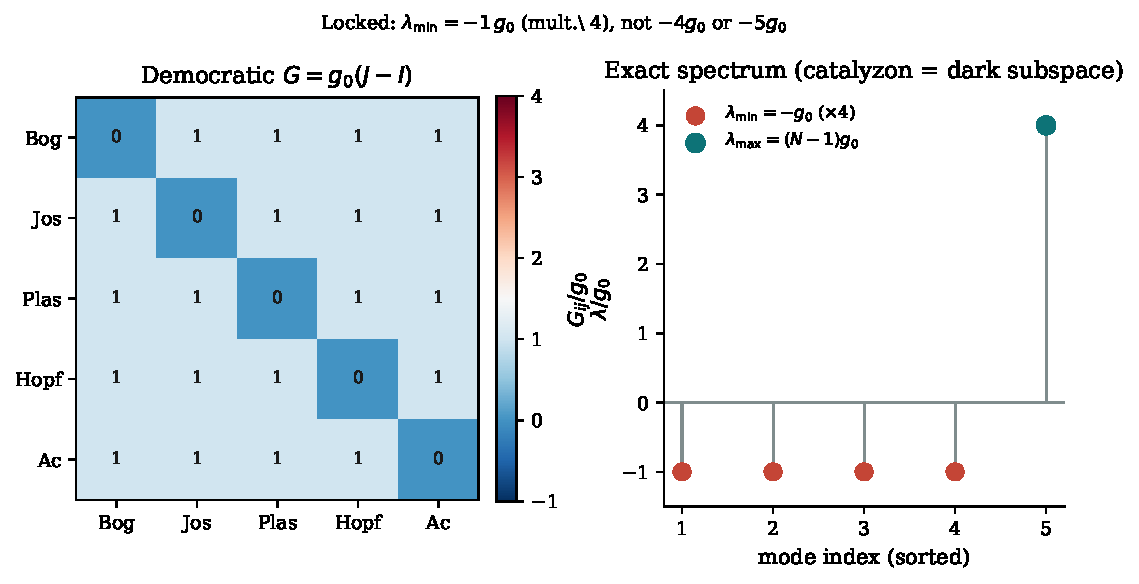
\includegraphics[width=0.95\textwidth]{figures/five_mode_coupling_matrix.pdf}
\caption{\textbf{Five-mode coupling matrix and eigenvalue spectrum.} (\textit{Left}) Democratic coupling $G=g_0(J-I)$ with zero diagonal and $\operatorname{Tr} G=0$. (\textit{Right}) Exact spectrum: dark/catalyzon subspace $\lambda_{\min}=-g_0$ (multiplicity~$N-1$) and bright mode $\lambda_{\max}=(N-1)g_0$.}
\label{fig:hybridization}
\end{figure}

\begin{figure}[htbp]
\centering
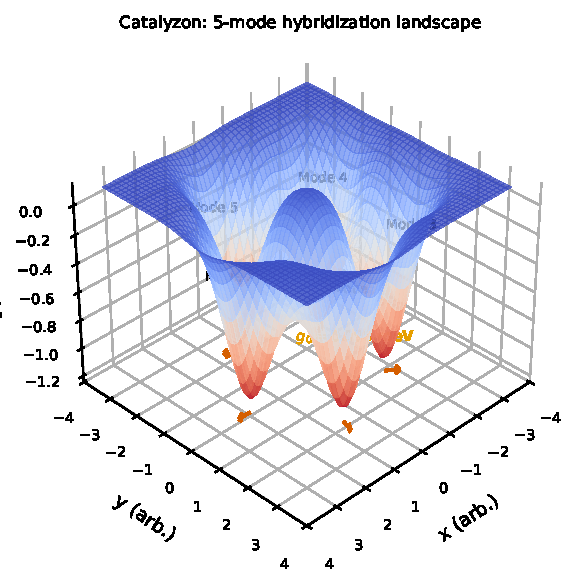
\includegraphics[width=0.75\textwidth]{figures/catalyzon_formation_3d.pdf}
\caption{\textbf{Catalyzon formation.} (\textit{Left}) Schematic collective-mode dispersions meeting at the two-particle threshold. (\textit{Right}) Eigenvalue splitting versus $g_0$: four-fold dark multiplet at $\lambda_{\min}=-g_0$ and bright mode at $\lambda_{\max}=4g_0$ ($N=5$). Catalyzon hybridization is a parallel channel to the static fold and to truncated GPE dynamics.}
\label{fig:catalyzon3d}
\end{figure}

\begin{figure}[htbp]
\centering
\includegraphics[width=0.92\textwidth]{figures/catalyzon_dark_modes.pdf}
\caption{\textbf{Catalyzon dark-mode basis.} Orthonormal Helmert vectors spanning the sum-zero subspace of the democratic coupling matrix (eigenvalue $\lambda_{\min}=-g_0$).}
\label{fig:dark_modes}
\end{figure}

The model hybridizes five long-wavelength collective modes at the two-particle threshold $\omega_0 = 2\Delta/\hbar$:

\begin{enumerate}
    \item \textbf{Bogoliubov out-of-phase (amplitude) mode}: Higgs-like oscillation of the condensate magnitude $|\Psi|$. In a BCS-BEC crossover system, this mode corresponds to pair-breaking excitations. Frequency at $k=0$ is $\omega_H = 2\Delta$ (threshold condition). This mode modulates the local gap $\Delta(\mathbf{r}, t)$ and couples to all other modes through the nonlinear condensate dynamics.

    \item \textbf{Josephson plasma mode}: Relative-phase oscillation between adjacent \TEVC{} layers, $\theta_j - \theta_{j+1}$ where $j$ labels layers. Frequency $\omega_J = \sqrt{2 E_J E_C/\hbar^2}$ where $E_J$ is Josephson coupling and $E_C$ is charging energy. For \MATBG{} at twist $\theta \approx 1.1^\circ$ with $N=5$ layers, interlayer tunneling produces $E_J \sim 0.1$ meV and capacitive charging gives $E_C \sim 1$ meV, yielding $\omega_J \sim 2\Delta/\hbar$ (near-resonant).

    \item \textbf{Flat-band plasmon}: Collective density oscillation within the moiré unit cell, $\delta n(\mathbf{r}, t) = n_0 e^{i(\mathbf{q} \cdot \mathbf{r} - \omega t)}$. Flat-band dispersion with bandwidth $W \ll E_F$ produces a plasmon mode $\omega_{\text{pl}}^2 = (4\pi e^2 n_0 / m^*) f_q$ where $f_q$ is a geometric form factor and $m^*$ is the flat-band effective mass. For long-wavelength $q \ll K_M$, $\omega_{\text{pl}} \sim 2\Delta/\hbar$.

    \item \textbf{Hopfion field mode}: Small deformations of the topological texture, parameterized as $\hat{\mathbf{n}}(\mathbf{r}, t) = \hat{\mathbf{n}}_0(\mathbf{r}) + \delta \hat{\mathbf{n}}(\mathbf{r}, t)$ where $\hat{\mathbf{n}}_0$ is the static hopfion solution. These are analogous to spin-wave excitations in magnets but with nontrivial topology. Restoring forces from $\mathcal{F}_{\text{Skyrme}}$ (higher-derivative stabilization) produce a characteristic frequency $\omega_{\text{hopf}} \sim \sqrt{\kappa_S / (m^* R^2)} \sim 2\Delta/\hbar$ for ring radius $R \sim 50$ nm.

    \item \textbf{Bogoliubov acoustic (Goldstone) mode}: Phase mode $\theta(\mathbf{r}, t)$ with linear dispersion $\omega = c_s k$ at long wavelength. At $k=0$ this mode has zero energy (Goldstone mode of broken $U(1)$ symmetry). However, at finite $k^* = 2\Delta/(\hbar c_s)$, $\omega(k^*) = 2\Delta/\hbar$, bringing it into resonance with the other four modes.
\end{enumerate}

\subsection{Resonance Condition and Mode Degeneracy}

In the resonant model the five modes are taken as accidentally degenerate at $\omega_0 = 2\Delta/\hbar$ for the wavevector $q^*$ of Section~\ref{sec:phonons}. The degeneracy is not symmetry-protected; it is a working assumption of the five-mode algebra. Linearization of truncated \TQGL{} does not produce five Goldstone modes, as discussed above.

Zero-point fluctuations of the electromagnetic field (Casimir modes with $\mathcal{F}(x) = \Flock$, Section~\ref{sec:casimir}) and phononic field (flat phonon bands, Section~\ref{sec:phonons}) introduce vacuum-mediated interactions between these modes. These interactions are off-diagonal: they do not shift individual mode frequencies (no diagonal $G_{ii}$ terms) but instead hybridize the modes through pair-wise couplings $G_{ij}$ for $i \neq j$.

\subsection{Coupling Matrix Structure}

The five-mode Hamiltonian near $\omega_0$ is
\begin{equation}
H = \sum_{i=1}^5 \hbar \omega_0 a_i^\dagger a_i + \sum_{i<j} G_{ij} (a_i^\dagger a_j + a_j^\dagger a_i),
\end{equation}
where $a_i^\dagger, a_i$ are creation/annihilation operators for mode $i$, and $G \in \mathbb{R}^{5 \times 5}$ is the symmetric coupling matrix. By construction:
\begin{itemize}
    \item $G_{ii} = 0$ (no self-energy corrections at resonance);
    \item $\operatorname{Tr} G = 0$ (sum rule from charge neutrality and momentum conservation);
    \item $G_{ij}$ mediated by vacuum field correlators $\langle \phi_{\text{ZPF}}(\mathbf{r}) \phi_{\text{ZPF}}(\mathbf{r}')\rangle$.
\end{itemize}

Diagonalizing $H$ yields eigenvalues $\hbar \omega_0 + \lambda_i$ where $\{\lambda_i\}_{i=1}^5$ are eigenvalues of $G$. For the democratic coupling $G=g_0(J_N-I_N)$ the spectrum is exact: $\lambda_{\max}=(N-1)g_0$ (multiplicity~1; bright/in-phase) and $\lambda_{\min}=-g_0$ (multiplicity~$N-1$; dark/sum-zero). The catalyzon corresponds to this dark subspace. 

\begin{theorem}[Catalyzon Formation Criterion]
Let $G \in \mathbb{R}^{5\times 5}$ be symmetric with $G_{ii} = 0$ for all $i$, $\operatorname{Tr} G = 0$, and $G \neq 0$. Then at least one eigenvalue of $G$ is strictly negative, and the catalyzon gap satisfies
\begin{equation}
\boxed{\Delta_{\text{cat}} = \Delta_{\text{ex}} + \lambda_{\min} < \Delta_{\text{ex}}.}
\end{equation}
\end{theorem}

\begin{proof}
Symmetry of $G$ implies eigenvalues $\{\lambda_i\}_{i=1}^5$ are real and $\sum_i \lambda_i = \operatorname{Tr} G = 0$. The Frobenius norm satisfies $\|G\|_F^2 = \sum_{ij} G_{ij}^2 = \sum_i \lambda_i^2 > 0$ since $G \neq 0$, so not all $\lambda_i$ vanish. Combined with $\sum_i \lambda_i = 0$ and not all $\lambda_i = 0$, there exist eigenvalues of both signs; in particular $\lambda_{\min} < 0$.
\end{proof}

\subsection{Physical Interpretation and Magnitude}

The catalyzon eigenvector $|\text{cat}\rangle = \sum_{i=1}^5 c_i |i\rangle$ is a coherent superposition of the five modes with amplitudes $c_i$ determined by diagonalizing $G$. The negative eigenvalue $\lambda_{\min} < 0$ represents a \textit{binding energy}: vacuum-mediated interactions lower the energy of this particular superposition below the uncoupled resonance.

From the locked vacuum $E_{\mathrm{vac}}=\Evac$ with $g_0=\lambda^\star E_{\mathrm{vac}}=\gzerostar$, the democratic dark eigenvalue is $|\lambda_{\min}|=g_0$, yielding
\begin{equation}
\Delta_{\text{cat}} = \Delta_{\text{ex}}-g_0^\star = \Deltacat.
\end{equation}
This is a \pctcat{} reduction from the bare exchange gap $\Delta_{\text{ex}} = \Deltaex$ on the democratic channel, distinct from the static fold reduction at $\lambda^\star$. At the fold edge the same identification gives $g_0=\gzerofold=\Delta_c$ (\pctcatfold). The catalyzon thus provides a lower-energy pathway for barrier crossing, parallel to the fold.

\subsection{Role in Quantum Vacuum Catalyzation}

The catalyzon is the microscopic agent of barrier reduction in \QVC{}. When the system attempts to cross the Mexican-hat potential barrier (Section~\ref{sec:tqgl}), it can do so by:
\begin{enumerate}
    \item \textbf{Bare thermal activation}: Overcoming barrier $\Delta_{\text{ex}}$ through thermal fluctuations, with rate $\Gamma_{\text{thermal}} \propto e^{-\Delta_{\text{ex}}/k_B T}$.
    \item \textbf{Quantum tunneling}: Tunneling through the barrier with WKB suppression $\Gamma_{\text{tunnel}} \propto e^{-S_{\text{inst}}/\hbar}$ where $S_{\text{inst}}$ is the instanton action.
    \item \textbf{Catalyzon-mediated crossing}: Accessing the lower-gap state $\Delta_{\text{cat}}$, with enhanced rate $\Gamma_{\text{QVC}} \propto e^{-\Delta_{\text{cat}}/k_B T}$ (thermal) or reduced tunneling action.
\end{enumerate}

At sub-Kelvin temperatures ($T \ll \Delta_{\text{ex}}/k_B \sim 7$ K), thermal activation is negligible and quantum tunneling dominates. The catalyzon reduces the effective barrier from $\Delta_{\text{ex}}$ to $\Delta_{\text{cat}}$, exponentially enhancing the tunneling probability.

\subsection{Scope of the five-mode model}

The five-mode Hamiltonian is a resonant model for $\mathrm{Spec}(G)$, not a Goldstone theorem. Truncated \TQGL{} about the hopfion supplies one discrete Goldstone (Section~\ref{sec:lin_tqgl}). Democratic $\mathrm{Spec}(G)$ is exact algebra at the bridge value $g_0^\star$; Wigner--Seitz $K_0$ and Hessian overlaps $G^{(H)}$ are computed kernels, neither equal to $g_0(J-I)$ in meV. A Cartan-torsion origin for $G_{ij}$ (hypothesis H-TOR1) is not evaluated here. Theorem~6.1 still guarantees that any nonzero off-diagonal vacuum coupling of the democratic algebra produces a dark eigenvalue $\lambda_{\min}=-g_0$. That statement concerns $\mathrm{Spec}(G)$, not the number of hopfion soft modes.

\section{Topological Ginzburg-Landau Functional}
\label{sec:tqgl}

The \QVC{} low-energy field theory is the Topological Ginzburg-Landau (\TQGL) functional:
\begin{equation}
\mathcal{F}[\Psi, \mathbf{a}] = \mathcal{F}_{\text{bulk}} + \mathcal{F}_{\text{CS}} + \mathcal{F}_{\text{Berry}} + \mathcal{F}_{\text{ZPF}} + \mathcal{F}_{\text{Skyrme}},
\end{equation}
with
\begin{align}
\mathcal{F}_{\text{bulk}} &= \int \mathrm{d}^2 r \left[ \alpha |\Psi|^2 + \frac{\beta}{2} |\Psi|^4 + \kappa |\nabla \Psi|^2 \right], \\
\mathcal{F}_{\text{CS}} &= \frac{k}{4\pi} \int \mathbf{a} \wedge \mathrm{d}\mathbf{a}, \quad k = 2N, \\
\mathcal{F}_{\text{Berry}} &= \int \mathrm{d}^2 r \, \Omega(\mathbf{k}) \cdot \mathbf{j}(\mathbf{r}), \\
\mathcal{F}_{\text{ZPF}} &= -\lambda \int \mathrm{d}^2 r \, A_{\text{ZPF}}(\mathbf{r}) |\Psi(\mathbf{r})|^2, \\
\mathcal{F}_{\text{Skyrme}} &= \kappa_S \int \mathrm{d}^2 r \, |\nabla^2 \Psi|^2.
\end{align}
\begin{figure}[htbp]
\centering
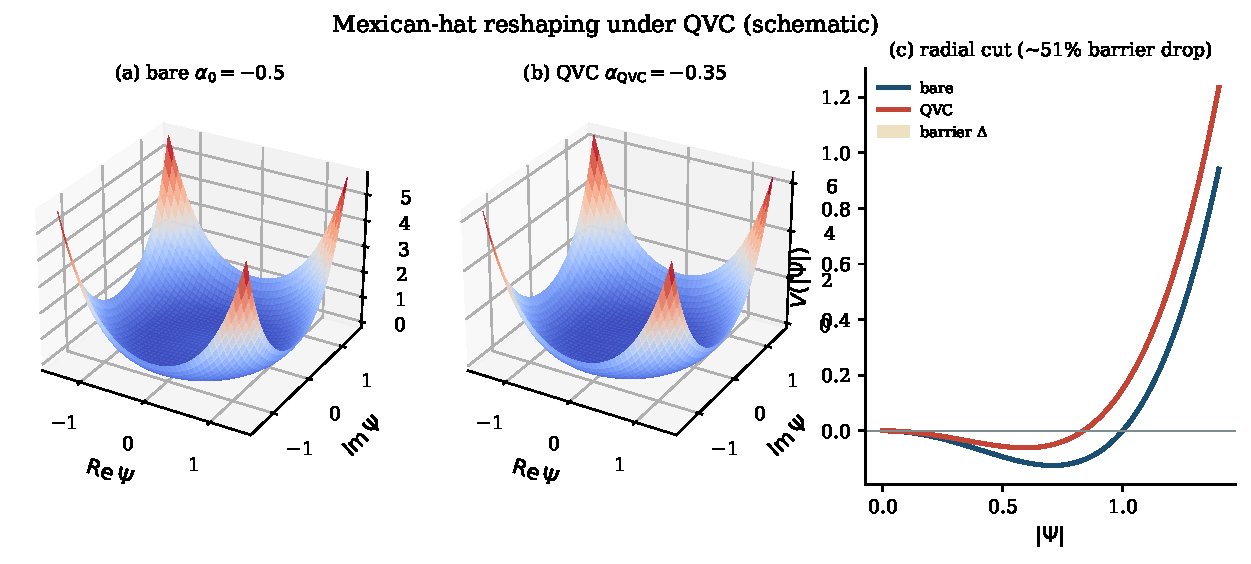
\includegraphics[width=0.75\textwidth]{figures/mexican_hat_3d_catalyzon.pdf}
\caption{\textbf{Mexican-hat potential reshaping (3D visualization).} (\textit{Left}) Bare quadratic-quartic $V(\rho)=\alpha_{\mathrm{GL}}\rho^2+(\beta/2)\rho^4$ of the Track~A family (Section~\ref{sec:l1_dictionary}). (\textit{Center}) The same potential with Landau mass tracking the catalyzon gap $\Delta_{\mathrm{cat}}=\Deltacat$. (\textit{Right}) Radial cut: well-depth reduction $B_{\mathrm{cat}}/B_0=(\Delta_{\mathrm{cat}}/\Delta_0)^2$ is \hatbarrier{} from the matched $V(\rho)$, while the parallel catalyzon pathway is the \pctcat{} gap reduction $\Delta_{\mathrm{ex}}\to\Delta_{\mathrm{cat}}$.}
\label{fig:mexican}
\end{figure}

$\mathcal{F}_{\text{bulk}}$ is the conventional Ginzburg-Landau Mexican-hat potential fixing the condensate amplitude (Fig.~\ref{fig:mexican}). $\mathcal{F}_{\text{CS}}$ is a Chern-Simons term for the emergent gauge field $\mathbf{a}$ coupled to the condensate phase; at locked level $k=2N$ the \emph{dictionary} Hall response of the uncatalyzed state is $\sigma_{xy}=(k/2)e^2/h=N e^2/h$, with step~\eqref{eq:dsigma_lock}; this is not the unique Wen/Laughlin evaluation $\sigma_{xy}=k e^2/h$ of $\frac{k}{4\pi}\int\mathbf{a}\wedge\mathrm{d}\mathbf{a}$ (Remark~\ref{rem:cs_convention})\cite{Laughlin1983,Wen1995}. $\mathcal{F}_{\text{Berry}}$ threads the band Berry curvature through the condensate, ensuring that the topology of the underlying electrons is inherited by the \TEVC{} order parameter\cite{Xiao2010,Qi2011}. $\mathcal{F}_{\text{ZPF}}$ encodes the vacuum coupling explicitly: where the local zero-point amplitude is large, the condensate is favored. Finally, the higher-derivative Skyrme term $\mathcal{F}_{\text{Skyrme}}$ stabilizes finite-size topological textures against Derrick collapse\cite{Faddeev1997,Sutcliffe2007}. The matched numerical values of $\alpha_{\mathrm{GL}}$, $\beta$, $\kappa_{\mathrm{GL}}$, $\lambda^\star$, $g_0$, and the Hall step are collected in Section~\ref{sec:l1_dictionary}.

\section{Matched L1 coefficients, lengths, and catalyzon scale}
\label{sec:l1_dictionary}

The preceding sections introduce the frozen-cavity bridge, the democratic catalyzon, and the bulk \TQGL{} functional. Those objects share symbols---lengths, Landau coefficients, a vacuum coupling $g_0$, a Hall step, a retardation factor, and an analogue horizon radius---that must not be identified across distinct geometric settings. This section records one convention for each quantity. Fold, catalyzon, and truncated Gross--Pitaevskii dynamics remain independent channels. Holographic and torsion constructions are not used to derive $G_{ij}$ or $\kappa_{\mathrm{GL}}$. The matching $T_H=T^*$ (hypothesis H-HAWK1) fixes $R_{\mathrm{WS}}$.

\subsection{Length dictionary}
\label{sec:length_dict}

The frozen-cavity geometry identifies the fat-torus tube with the Ginzburg--Landau healing length,
\begin{equation}
a_H = r = \aHlock
\end{equation}
A second length is the phonon (Bogoliubov) healing constructed from the same package constants that enter the gap map,
\begin{equation}
\xi_{\mathrm{ph}} = \frac{\hbar c_s}{\Delta_0} = \xiph
\end{equation}
These two lengths are not interchangeable: $a_H$ is the cavity minor radius and the GPE core scale; $\xi_{\mathrm{ph}}$ is the scale on which $\Delta_0$ and $\hbar c_s$ produce a dimensionless ratio of order one.

Retardation is defined from the causal phonon propagator by the algebraic identity
\begin{equation}
\eta_{\mathrm{ret}} = \frac{2\Delta_0\xi}{\hbar c_s}
\label{eq:eta_ret_lock}
\end{equation}
Substituting the two lengths of this dictionary yields the pair
\begin{equation}
\eta_{\mathrm{ret}}(a_H)=\etaretaH,\qquad
\eta_{\mathrm{ret}}(\xi_{\mathrm{ph}})=\etaretph.
\end{equation}
The second evaluation is an identity: $\xi_{\mathrm{ph}}=\hbar c_s/\Delta_0$ converts Eq.~\eqref{eq:eta_ret_lock} into $\eta_{\mathrm{ret}}=2$. An alternate coherence length $\xi=\xialt$ produces $\eta_{\mathrm{ret}}\approx\etaretalt$. Table~\ref{tab:length_dict} records the three evaluations.

\begin{table}[htbp]
\centering
\caption{Length dictionary on the frozen cavity. The retardation identity is Eq.~\eqref{eq:eta_ret_lock}.}
\begin{tabular}{llll}
\hline
\textbf{Length} & \textbf{Value} & $\eta_{\mathrm{ret}}$ & \textbf{St.} \\
\hline
$a_H=r$ (GL/GPE) & $\aHlock$ & $\etaretaH$ & L \\
$\xi_{\mathrm{ph}}=\hbar c_s/\Delta_0$ & $\xiph$ & $\etaretph$ & D \\
$\xi$ (alternate) & $\xialt$ & $\etaretalt$ & Alt \\
\hline
\end{tabular}
\label{tab:length_dict}
\end{table}

\subsection{Locked kinematics: mass, frequencies, two velocities}
\label{sec:kinematics_dict}

The gradient weight $\kappa_{\mathrm{GL}}=\Delta_0 a_H^2$ is $\hbar^2/(2m^*)$, so
\begin{equation}
\frac{m^*}{m_e}=\frac{\hbar^2/(2m_e)}{\kappa_{\mathrm{GL}}}=\mstaroverme
\end{equation}
The healing identification $a_H=\hbar/\sqrt{2m^*\Delta_0}$ with locked $a_H=\aHlock$ therefore requires $m^*\approx m_e$, not $0.4\,m_e$.

Package $\hbar c_s=\hbarcs$ converts to $c_s=\csBog$. This velocity enters the Casimir prefactor, the gap map, retardation~\eqref{eq:eta_ret_lock}, and the Goldstone resonance $k^*=2\Delta/(\hbar c_s)$. Independently, graphene's longitudinal acoustic speed is $c_{\mathrm{LA}}=\cLA$ and locates the moiré-zone wavevector $q^*=\omega_0/c_{\mathrm{LA}}$. The two speeds are not identified.

Cyclic frequencies $\nu=\omega/(2\pi)$ at $\omega=2\Delta/\hbar$ are $\nu_{\mathrm{GPE}}=\nuGPE$ for the GPE drive $\Delta=\Delta_0$ and $\nu^\star=\nuStar$ for the working gap $\Delta^\star$. Angular $\omega_0(\Delta_0)=\omegaGPEps$. At $\Delta^\star$ the graphene-LA kinematics give $q^*=\qstarLA$, $\lambda_{\mathrm{res}}=2\pi/q^*=\lamresLA$, and $q^*/K_M=\qoverKM$ with $K_M=4\pi/(3\lambda_M)$. The Bogoliubov wavelength at the same $\Delta^\star$ is $\lamresCS$. The Vakulenko--Kapitansky comparison uses $E_{\mathrm{vac}}$: $N^{-3/4}\approx 0.299$ implies $C > \Cvkmin$.

\subsection{Track A Ginzburg--Landau coefficients}
\label{sec:gl_dict}

The bulk functional of Section~\ref{sec:tqgl} and the two-sector split of Section~\ref{sec:vortex_rg} employ a Landau mass $\alpha_{\mathrm{GL}}$, a quartic $\beta$, and a gradient weight $\kappa_{\mathrm{GL}}$, together with a participation $\lambda$ that feeds the gap-map coupling $\alpha$ of Section~\ref{sec:bridge}. These are distinct objects. The gap-map coupling is dimensionless,
\begin{equation}
\alpha=\lambda\frac{E_{\mathrm{vac}}}{\Delta_0},
\end{equation}
and at the working point equals $\alpha^\star=\alphastar$. The Landau mass is matched to the bare exchange gap of the truncated GPE,
\begin{equation}
\alpha_{\mathrm{GL}}=-\Delta_0=\alphaGL
\end{equation}
so that $|\alpha_{\mathrm{GL}}|=\Delta_0$ and $\alpha_{\mathrm{GL}}$ is not the number $\alpha^\star$. The gradient weight follows from the healing identification $a_H=r$ in the kinetic coefficient $\hbar^2/(2m^*)$,
\begin{equation}
\kappa_{\mathrm{GL}}=\Delta_0 a_H^2=\kappaGL
\end{equation}
Hence $m^*=\hbar^2/(2\kappa_{\mathrm{GL}})=\mstaroverme\,m_e$. This $\kappa_{\mathrm{GL}}$ is not the holographic $\gamma_{\mathrm{QM}}$ of Section~\ref{sec:holographic_dict}; that coefficient is an L3 matching and is not imported into Track~A.

The quartic is matched so that the Mexican-hat vacuum manifold sits on the hopfion density of the truncated solver. On the ring-weighted initial condition of \texttt{hopfion\_initial} (box $L=200$\,nm, $n_0=1$, core depletion $0.10$, noise-free) one finds $n_{\mathrm{ref}}=\nrefhopf$, and therefore
\begin{equation}
\beta=\frac{\Delta_0}{n_{\mathrm{ref}}}=\betaGL
\end{equation}
The GPE cubic-quintic potential used in the $1$\,ps integrator is the related but not identical pair $\alpha_{\mathrm{nl}}=-\Delta_0$, $\beta_{\mathrm{nl}}=\Delta_0/n_0$ with dimensionless $n_0=1$; $n_{\mathrm{ref}}$ is the live-gap denominator of Section~\ref{sec:dynamics}. Participation in the dictionary is the working value $\lambda=\lambda^\star=\lstar$, with $\lambda_{\mathrm{fold}}=\lfold$ the edge of the physical fold branch.

The Skyrme coefficient that stabilizes finite-size textures against Derrick collapse is not derived from a microscopic Hubbard model. A Faddeev--Skyrme balance at the locked tube scale $a_H$ gives the estimate $\kappa_S\sim\kappa_{\mathrm{GL}}a_H^2=\Delta_0 a_H^4=\kappaSansatz$. Table~\ref{tab:gl_dict} collects the Track~A card.

\begin{table}[htbp]
\centering
\caption{Track A Ginzburg--Landau coefficients. The gap-map $\alpha$ is dimensionless; $\alpha_{\mathrm{GL}}$ and $\beta$ are energies. Holographic $\gamma_{\mathrm{QM}}$ is not $\kappa_{\mathrm{GL}}$.}
\begin{tabular}{llll}
\hline
\textbf{Symbol} & \textbf{Value} & \textbf{Meaning} & \textbf{St.} \\
\hline
$\alpha^\star$ & $\alphastar$ & Gap-map $\lambda^\star E_{\mathrm{vac}}/\Delta_0$ & D \\
$\alpha_{\mathrm{GL}}$ & $\alphaGL$ & Landau mass, $|\alpha_{\mathrm{GL}}|=\Delta_0$ & M \\
$\kappa_{\mathrm{GL}}$ & $\kappaGL$ & $\Delta_0 a_H^2$ with $a_H=r$ & D \\
$m^*/m_e$ & $\mstaroverme$ & $\hbar^2/(2\kappa_{\mathrm{GL}})$ & D \\
$\lambda^\star$ & $\lstar$ & Working participation & L \\
$\beta$ & $\betaGL$ & $\Delta_0/n_{\mathrm{ref}}$ on hopfion IC & M \\
$n_{\mathrm{ref}}$ & $\nrefhopf$ & Ring-weighted hopfion density & C \\
$\kappa_S$ & $\kappaSansatz$ & Derrick estimate at tube scale & A \\
\hline
\end{tabular}
\label{tab:gl_dict}
\end{table}

\subsection{Catalyzon scale \texorpdfstring{$g_0=\lambda E_{\mathrm{vac}}$}{g0 = lambda E\_vac}}
\label{sec:g0_dict}

If the same vacuum that feeds the fold also hybridizes the five long-wavelength modes of Section~\ref{sec:catalyzon}, the off-diagonal coupling is the bridge identification
\begin{equation}
g_0=\lambda E_{\mathrm{vac}}.
\label{eq:g0_bridge}
\end{equation}
At the working point $\lambda^\star$ this is $g_0^\star=\gzerostar$, so the democratic dark eigenvalue $\lambda_{\min}=-g_0$ produces
\begin{equation}
\Delta_{\mathrm{cat}}=\Delta_{\mathrm{ex}}-g_0^\star=\Deltacat
\end{equation}
(\pctcat{} of $\Delta_{\mathrm{ex}}=\Deltaex$). At the fold edge $\lambda_{\mathrm{fold}}$ one has $g_0=\lambda_{\mathrm{fold}}E_{\mathrm{vac}}=\gzerofold=\Delta_c$, a \pctcatfold{} catalyzon reduction. Both evaluations are parallel to the static fold: $\Delta^\star=\Deltastar$ at $\lambda^\star$ is an amplitude-map number, not a stacked correction to $\Delta_{\mathrm{cat}}$. The working vacuum scale is $g_0^\star$; a coupling larger than $E_{\mathrm{vac}}$ is not a participation of the locked vacuum.

\subsection{Mexican-hat barrier from $V(\rho)$}
\label{sec:mexican_dict}

The bulk potential of Track~A is the quadratic-quartic family
\begin{equation}
V(\rho)=\alpha_{\mathrm{GL}}\,\rho^2+\frac{\beta}{2}\rho^4,
\label{eq:Vrho}
\end{equation}
with $\alpha_{\mathrm{GL}}$ and $\beta$ from Table~\ref{tab:gl_dict}. The vacuum manifold sits at $\rho^2=|\alpha_{\mathrm{GL}}|/\beta=n_{\mathrm{ref}}$, and the well depth measured from $\rho=0$ is
\begin{equation}
B=\frac{\alpha_{\mathrm{GL}}^2}{2\beta}=\frac{\Delta_0\,n_{\mathrm{ref}}}{2}.
\end{equation}
On the catalyzon channel the Landau mass tracks the dressed gap, $\alpha_{\mathrm{GL}}\to-\Delta_{\mathrm{cat}}$, at the same $\beta$. The well-depth ratio is then independent of $n_{\mathrm{ref}}$,
\begin{equation}
\frac{B_{\mathrm{cat}}}{B_0}=\left(\frac{\Delta_{\mathrm{cat}}}{\Delta_0}\right)^2,
\end{equation}
which evaluates to a \hatbarrier{} reduction. Figure~\ref{fig:mexican_matched} shows the radial cuts of Eq.~\eqref{eq:Vrho} at $\alpha_{\mathrm{GL}}=-\Delta_0$ and $\alpha_{\mathrm{GL}}=-\Delta_{\mathrm{cat}}$. This is the barrier of the matched potential, not a schematic pair of Landau masses.

\begin{figure}[htbp]
\centering
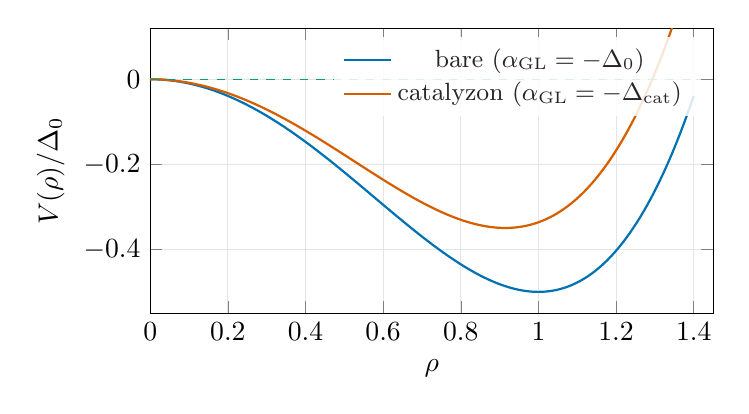
\begin{tikzpicture}
\begin{axis}[
  width=0.72\linewidth,
  height=5.2cm,
  xlabel={$\rho$},
  ylabel={$V(\rho)/\Delta_0$},
  xmin=0, xmax=1.45,
  ymin=-0.55, ymax=0.12,
  legend style={font=\small, at={(0.97,0.97)}, anchor=north east, draw=none, fill=white, fill opacity=0.85},
  grid=major, grid style={gray!20},
  clip=true,
]
\addplot[oiBlue, thick, domain=0:1.4, samples=200]
  {-1.0*x^2 + 0.5*x^4};
\addlegendentry{bare ($\alpha_{\mathrm{GL}}=-\Delta_0$)}
\addplot[oiVerm, thick, domain=0:1.4, samples=200]
  {-(0.5018/0.600)*x^2 + 0.5*x^4};
\addlegendentry{catalyzon ($\alpha_{\mathrm{GL}}=-\Delta_{\mathrm{cat}}$)}
\addplot[oiGreen, dashed, domain=0:1.4, samples=2] {0};
\end{axis}
\end{tikzpicture}
\caption{\textbf{Matched Mexican-hat radial cuts.} Equation~\eqref{eq:Vrho} in units of $\Delta_0$, with the Track~A quartic $\beta$ scaled out of the dimensionless plot. Well-depth reduction $B_{\mathrm{cat}}/B_0=(\Delta_{\mathrm{cat}}/\Delta_0)^2$ is \hatbarrier{}. The catalyzon pathway $\Delta_{\mathrm{ex}}\to\Delta_{\mathrm{cat}}$ remains the parallel \pctcat{} gap reduction of Section~\ref{sec:g0_dict}.}
\label{fig:mexican_matched}
\end{figure}

\subsection{Hall convention}
\label{sec:hall_dict}

A single Chern--Simons \emph{dictionary} is used throughout. The topological term in the \TQGL{} functional is
\begin{equation}
\mathcal{F}_{\mathrm{CS}}=\frac{k}{4\pi}\int\mathbf{a}\wedge\mathrm{d}\mathbf{a},\qquad k=2N,
\end{equation}
and the lens-space identification of Section~\ref{sec:lens_space_proof} is $Q_H=1/N$. These two statements are independent locks; their product $k\,Q_H=2$ is algebra, not a pairing theorem that uniquely determines $k$ from $Q_H$ or conversely. The uncatalyzed Hall conductance of the condensate is
\begin{equation}
\sigma_{xy}=N\frac{e^2}{h}=\frac{k}{2}\frac{e^2}{h}.
\end{equation}
Each hopfion nucleation event changes that conductance by one step
\begin{equation}
\delta\sigma_{xy}=\frac{e^2}{2Nh}=\frac{Q_H e^2}{2h}=\frac{e^2}{kh}.
\label{eq:dsigma_lock}
\end{equation}
For $N=5$ this is $\delta\sigma_{xy}=\dsigmaH$. No second Hall formula is employed as a physics lock.

\begin{remark}[Dictionary versus textbook Chern--Simons]
\label{rem:cs_convention}
The usual continuum evaluation of $\frac{k}{4\pi}\int\mathbf{a}\wedge\mathrm{d}\mathbf{a}$ assigns Hall conductance $\sigma_{xy}=k\,e^2/h$~\cite{Laughlin1983,Wen1995}. At the locked level $k=2N$ that textbook reading would be $2N\,e^2/h$, which is \emph{not} the QVC lock. The paper uses $\sigma_{xy}=(k/2)e^2/h=N e^2/h$ as a dictionary convention so that the uncatalyzed condensate tracks $N$ layers and the step~\eqref{eq:dsigma_lock} remains $e^2/(2Nh)$. Likewise, textbook flux attachment at level $k$ is $\oint\mathbf{a}=2\pi/k=\pi/N$; the mean-field background integrated in Section~\ref{sec:cs_eom} is $a_\theta=Q_H/\rho$, whose holonomy is $2\pi Q_H=2\pi/N$. Both numbers are recorded. Neither is used to reset $k$, $Q_H$, $\sigma_{xy}$, or $\delta\sigma_{xy}$. The covariant stepper confirms the mean-field holonomy; it does not transport an edge and does not independently derive the Hall staircase.
\end{remark}

\subsection{Analogue horizon radius from \texorpdfstring{$T_H=T^*$}{TH = T*}}
\label{sec:rws_dict}

The Unruh--Visser acoustic metric of Section~\ref{sec:acoustic_hawking} has surface gravity $\kappa_{\mathrm{surface}}=2c_s/R_{\mathrm{WS}}$ and Hawking temperature $T_H=\hbar c_s/(\pi k_B R_{\mathrm{WS}})$. Hypothesis H-HAWK1 is the matching condition $T_H=T^*$, which inverts for the Wigner--Seitz radius
\begin{equation}
R_{\mathrm{WS}}=\frac{\hbar c_s}{\pi k_B T^*}=\RwsMatch
\label{eq:Rws_match}
\end{equation}
using the Schwinger diagnostic $T^*=\Tstar$ constructed from $E_{\mathrm{pair}}=\Epair$ at $g_0^\star$. The same algebra at $T^*=285$\,mK returns $R_{\mathrm{WS}}=\RwsAlt$; that length is the matching at that temperature, not the present $T^*$. The Berry Monte Carlo ratio $R_{\mathrm{mean}}=\BerryR$ of Section~\ref{sec:berry_enhancement} is a dimensionless GUE/GOE comparison of $|\lambda_{\min}|$, not a radius, and is not $R_{\mathrm{WS}}$.

\subsection{Wigner--Seitz kernel \texorpdfstring{$G_{ij}$}{G\_ij}}
\label{sec:gij_dict}

Democratic $G=g_0(J_N-I_N)$ has the exact spectrum $\lambda_{\max}=(N-1)g_0$ (multiplicity~$1$) and $\lambda_{\min}=-g_0$ (multiplicity~$N-1$) at the bridge scale $g_0^\star$. That algebra does not evaluate matrix elements and is not inserted into $G_{ij}$. Two computed kernels share the Macdonald function $K_0(|\mathbf{r}-\mathbf{r}'|/\xi_K)$ with $\xi_K=R=50$\,nm and set $G_{ii}=0$.

The Gaussian construction places five profiles of width $\sigma\approx 0.18\,\lambda_M$ on a regular pentagon inside the moir\'e Wigner--Seitz hexagon. The output is Hermitian and traceless, with $\lambda_{\min}<0$, mean off-diagonal $g_{0,\mathrm{eff}}=\gzeroeff$ in kernel units, and relative Frobenius distance $\relfroG$ from the democratic matrix at $\langle G_{\mathrm{off}}\rangle$. The eigenvalues are
\begin{equation}
\mathrm{Spec}(G_{K_0})\approx
\specGws:
\end{equation}
$\lambda_{\max}$ tracks $4g_{0,\mathrm{eff}}$, while the dark subspace is split by the pentagon-in-hexagon geometry rather than exactly four-fold. This $g_{0,\mathrm{eff}}$ is not the bridge energy $g_0^\star=\gzerostar$.

A ring-Fourier companion uses angular harmonics of the hopfion envelope, Wannier-transformed to $N$ localized packets on the locked torus. It returns $g_{0,\mathrm{eff}}=\gzeroeffring$ in kernel units and relative Frobenius distance $\relfroGring$, with
\begin{equation}
\mathrm{Spec}(G_{\mathrm{ring}})\approx
\specGring.
\end{equation}
Converting either $g_{0,\mathrm{eff}}$ to meV requires a prefactor that is not supplied by the overlap; the meV scale of the catalyzon remains the bridge value $g_0^\star$. Neither kernel is a torsion vertex (hypothesis H-TOR1 is left for a future three-dimensional Weitzenb\"ock quadrature; Section~\ref{sec:l1_closure}) nor a hand-inserted $J-I$.

\subsection{Lindblad window}
\label{sec:lindblad_dict}

The truncated GPE of Section~\ref{sec:dynamics} is kinetic plus cubic-quintic plus $V_{\mathrm{ZPF}}$ plus $V_{\mathrm{phonon}}$; Chern--Simons, Berry, and Skyrme terms are not discretised. A Lindblad dissipator is applied after each split step with phenomenological rates $\gamma_n=\gamma_{\phi}=1/\tau_{\mathrm{dec}}$. On the coherent $1$\,ps coupled-DCE window the integrator returns $\Delta_{\mathrm{live}}(1\,\mathrm{ps})=\Deltaliveone$ and $g^{(1)}=\goneps$. Combined number-plus-dephasing on that window is Table~\ref{tab:lindblad_1ps}.

\begin{table}[htbp]
\centering
\caption{Truncated GPE plus Lindblad on the $1$\,ps coupled-DCE window. Combined scan: $\gamma_n=\gamma_{\phi}=1/\tau_{\mathrm{dec}}$.}
\begin{tabular}{llll}
\hline
$\tau_{\mathrm{dec}}$ & $\Delta_{\mathrm{live}}$ & $g^{(1)}$ & St. \\
\hline
coherent & $\Deltaliveone$ & $\goneps$ & C \\
$5$\,ps & $\Deltataufive$ & $\gonetaufive$ & C \\
$20$\,ps & $\Deltatautwenty$ & $\gonetautwenty$ & C \\
$50$\,ps & $\Deltataufifty$ & $\gonetaufifty$ & C \\
\hline
\end{tabular}
\label{tab:lindblad_1ps}
\end{table}

Number-only damping at $\tau_{\mathrm{dec}}=5$\,ps gives $\Delta_{\mathrm{live}}=\Deltanumonly$ and $g^{(1)}=\gonumonly$; dephasing-only gives $\Delta_{\mathrm{live}}=\Deltadephonly$ and $g^{(1)}=\godephonly$. Number damping moves $\Delta_{\mathrm{live}}$; dephasing moves $g^{(1)}$. A $20$\,ps window with frozen $V_{\mathrm{ZPF}}$ (no DCE) isolates the rates: coherent $\Delta_{\mathrm{live}}=\Deltafrozencoherent$, $g^{(1)}=\gofrozencoherent$; at $\tau_{\mathrm{dec}}=5$, $20$, $50$\,ps the pairs are $(\Deltafrozentaufive,\ \gofrozentaufive)$, $(\Deltafrozentautwenty,\ \gofrozentautwenty)$, and $(\Deltafrozentaufifty,\ \gofrozentaufifty)$. The $\tau_{\mathrm{dec}}=5$\,ps frozen trajectory reaches $\Deltafrozentaufive$, below $\Delta_c=\Deltac$. That window is unphysical on the static branch and is not combined with $\Delta^\star$ or $\Delta_{\mathrm{cat}}$.

\section{Catalyzon linearization and algebraic closures}
\label{sec:l1_closure}

The dictionary of Section~\ref{sec:l1_dictionary} fixes the meV scale of the catalyzon by $g_0^\star=\lambda^\star E_{\mathrm{vac}}$. This section linearizes truncated \TQGL{} about the hopfion and records additional algebraic closures: a Chern--Simons covariant kinetic equation, a two-band quantum-metric stiffness on the physical fold branch, a Hubbard-scale matching, a Villain dualization with a finite-lattice $g(r)$, and the $S^3$ Hopf--Whitehead integral. A Cartan-torsion origin of $G_{ij}$ is not evaluated.

\subsection{Galerkin linearization about the hopfion}
\label{sec:lin_tqgl}

The truncated energy whose variation reproduces the Gross--Pitaevskii equation of Section~\ref{sec:dynamics} is
\begin{equation}
F[\psi]
=\int\mathrm{d}^2r\Bigl[
\kappa_{\mathrm{GL}}|\nabla\psi|^2
+\tfrac12\alpha_{\mathrm{nl}}n^2
+\tfrac13\beta_{\mathrm{nl}}n^3
+V_{\mathrm{ZPF}}n
\Bigr],
\label{eq:Ftrunc}
\end{equation}
with $n=|\psi|^2$, $\alpha_{\mathrm{nl}}=-\Delta_0$, $\beta_{\mathrm{nl}}=\Delta_0$, $\kappa_{\mathrm{GL}}=\Delta_0 a_H^2$, and $V_{\mathrm{ZPF}}=-E_{\mathrm{vac}}$ times the ring Gaussian. Chern--Simons, Berry, and Skyrme terms remain outside $F$, matching the stepper. A noise-free hopfion $\psi_0$ of Section~\ref{sec:dynamics} is the background. Infinitesimal $U(1)$ rotations $\psi\to e^{i\varepsilon}\psi$ leave~\eqref{eq:Ftrunc} invariant, so $\Phi_{\mathrm{G}}=i\psi_0$ is the Goldstone direction. A Galerkin basis orthonormalizes that Goldstone together with amplitude and phase packets $A(r)e^{in\theta}$ and $i\psi_0 e^{in\theta}$ for $n=0,\ldots,4$ on a $48^2$ periodic box.

The real Hessian $H_{ij}=\partial^2 F/\partial x_i\partial x_j$ along $\psi=\psi_0+\sum x_k\Phi_k$ is obtained by mixed central differences. Its spectrum on the locked freeze is
\begin{equation}
\mathrm{Spec}(H)\approx
\bigl(0.052,\,0.720,\,1.32,\,2.05,\,2.37,\,2.69,\,3.01,\,3.25,\,6.00,\,7.32\bigr)\,\mathrm{meV}
\label{eq:hess_spec}
\end{equation}
The lowest eigenvalue is the discrete Goldstone, lifted by the grid and the finite-difference step to $0.052$\,meV. The remaining nine directions are gapped by $\mathcal{O}(1)$\,meV. The truncated functional about a pinned ring therefore supports a single $U(1)$ Goldstone, not a five-fold Goldstone manifold. Figure~\ref{fig:hess_eigs} shows the stick spectrum.

\begin{figure}[htbp]
\centering
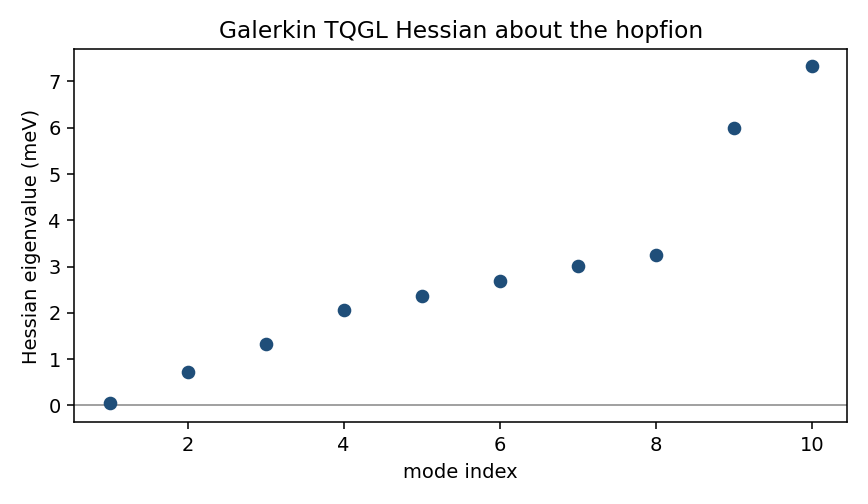
\includegraphics[width=0.72\linewidth]{closure_figs/fig_hessian_eigs.png}
\caption{\textbf{Galerkin Hessian of truncated \TQGL{} about the hopfion.} The isolated lowest eigenvalue is the discrete $U(1)$ Goldstone; the truncation does not produce five soft modes.}
\label{fig:hess_eigs}
\end{figure}

Off-diagonal entries of the amplitude block of $H$, with vanishing diagonal as in the catalyzon convention, define a Hessian coupling $G^{(H)}$ in meV. The mean off-diagonal is $g_{0,\mathrm{eff}}^{(H)}=\gzerohess$, of the same order as the bridge $g_0^\star$ but not equal to it (ratio $\approx 0.19$). Relative Frobenius distance to $g_0(J-I)$ at that mean is large: the Hessian coupling is not democratic. The meV catalyzon gap therefore remains $\Delta_{\mathrm{cat}}=\Delta_0-g_0^\star$ from Section~\ref{sec:l1_dictionary}; $G^{(H)}$ is a fluctuation pattern, not a replacement of the bridge.

\subsection{Dark versus bright envelopes}
\label{sec:hcat1}

On the Galerkin frequencies $\omega_k$ of~\eqref{eq:hess_spec}, a radiation kernel $\gamma_k=\gamma_0(\omega_k/\omega_{\mathrm{ref}})^2$ with $\gamma_0=0.05$\,ps$^{-1}$ assigns a larger decay rate to the stiffest mode. Evolving $c_k(t)=c_k(0)e^{-\gamma_k t}$ yields envelope times $\tau_{\mathrm{dark}}=\taudark$ and $\tau_{\mathrm{bright}}=\taubright$ (ratio $\tau_{\mathrm{dark}}/\tau_{\mathrm{bright}}\approx\tauratio$). Under that kernel the dark (sum-zero) weight outlives the bright eigenvalue, as expected if radiation damps stiffer modes more strongly. The kernel is an ansatz: uniform $\gamma$ would not distinguish the subspaces, and the existing GPE Lindblad of Section~\ref{sec:lindblad_dict} acts on $\psi$, not on a mode basis. Figure~\ref{fig:hcat1} shows the envelopes.

\begin{figure}[htbp]
\centering
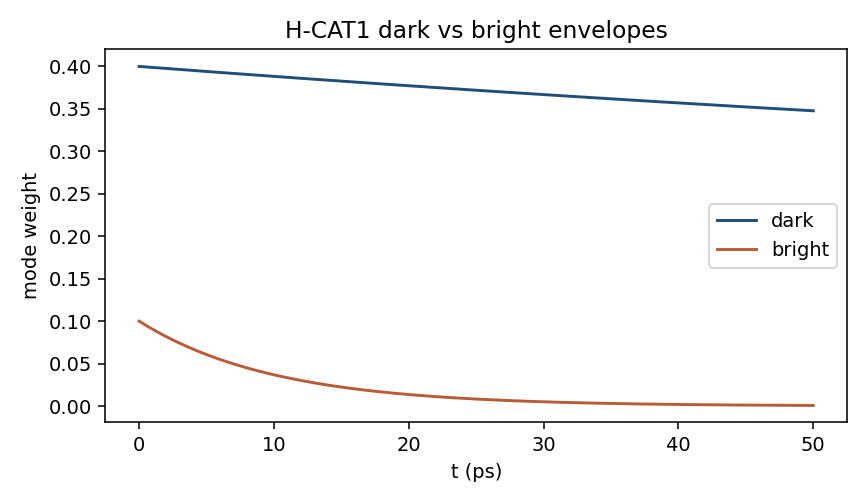
\includegraphics[width=0.72\linewidth]{closure_figs/fig_hcat1.png}
\caption{\textbf{Dark and bright envelopes.} Dark weight (smallest $|\omega|$) versus the brightest Galerkin mode with $\gamma\propto\omega^2$. The ratio of $1/e$ times is $\tauratio$ under that rate kernel.}
\label{fig:hcat1}
\end{figure}

\subsection{Torsion-overlap proxy}
\label{sec:htor1_comp}

The conjecture that democratic $G_{ij}$ arises as a Cartan torsion overlap on hopfion modes is not supported by the present evidence and is left open. A two-dimensional proxy using the phase Jacobian of $\psi_0$ as a Hopf-density stand-in $q_H$ and a weight $T=\lvert\nabla q_H\rvert$ produces overlaps $G_{ij}=\int\Phi_i^* T\Phi_j$ that are not near-democratic. A three-dimensional Weitzenb\"ock quadrature on true hopfion torsion is not performed. Democratic $\mathrm{Spec}(G)$ remains an algebraic identity; the Wigner--Seitz $K_0$ kernel of Section~\ref{sec:gij_dict} remains a distinct computed overlap; the bridge $g_0^\star$ is independent of this proxy. Figure~\ref{fig:htor1g} records the proxy matrix.

\begin{figure}[htbp]
\centering
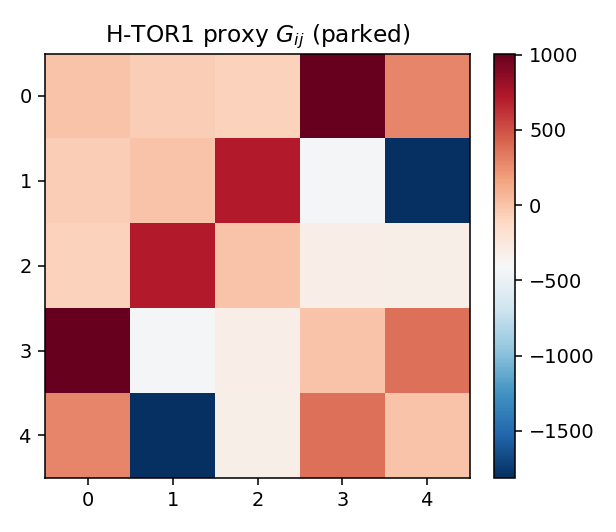
\includegraphics[width=0.55\linewidth]{closure_figs/fig_htor1_G.png}
\caption{\textbf{Two-dimensional torsion-proxy $G_{ij}$.} The pattern is not $g_0(J-I)$. A 3D Weitzenb\"ock quadrature is left for future development and is not used to set $G_{ij}$ or $g_0^\star$.}
\label{fig:htor1g}
\end{figure}

\subsection{Catalyzon spectral function}
\label{sec:Acat}

The mode spectral density
\begin{equation}
A_{\mathrm{cat}}(\omega)=\sum_k |c_k|^2\frac{\Gamma_k/\pi}{(\omega-\omega_k)^2+\Gamma_k^2}
\end{equation}
with $\Gamma_k=\hbar\gamma_k$ from the $\gamma\propto\omega^2$ kernel is shown in Fig.~\ref{fig:Acat}. It is the Galerkin-pole mix, not a tunneling lineshape. The two-particle phonon threshold $\omega_0=2\Delta/\hbar$ of Section~\ref{sec:phonons} remains a distinct energy from these Hessian poles.

\begin{figure}[htbp]
\centering
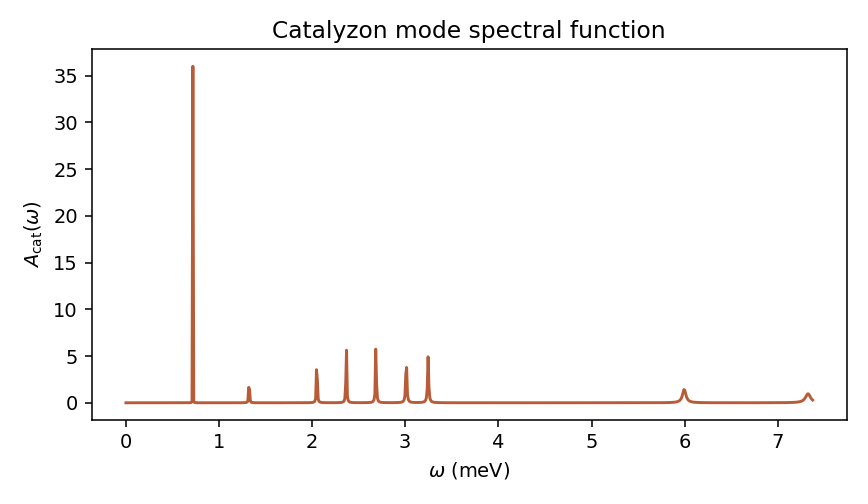
\includegraphics[width=0.72\linewidth]{closure_figs/fig_A_cat.png}
\caption{\textbf{Catalyzon mode spectral function.} Lorentzian mix of Galerkin Hessian poles. The bridge gap $\Delta_{\mathrm{cat}}$ is not read from this plot.}
\label{fig:Acat}
\end{figure}

\subsection{Chern--Simons constraint equation of motion}
\label{sec:cs_eom}

Level $k=2N$ is the dictionary lock. The mean-field constraint integrated here is the static connection $a_\theta=Q_H/\rho$, whose holonomy is $\Phi=2\pi Q_H=2\pi/N$. Textbook attachment $2\pi/k=\pi/N$ is a different convention and is not used to reset $k$ or $Q_H$ (Remark~\ref{rem:cs_convention}). The truncated kinetic operator $-\kappa\nabla^2$ is replaced by the covariant operator
\begin{equation}
H_{\mathrm{kin}}=\kappa(-i\nabla-a)^2
=\kappa\bigl[-\nabla^2+2ia\cdot\nabla+i(\nabla\cdot a)+|a|^2\bigr].
\label{eq:HkinCS}
\end{equation}
A Strang split advances half a covariant kinetic RK4 step, the local potential, then the other kinetic half-step, so $a$ sits inside the time stepper. On the locked torus the enclosed flux is $2\pi Q_H$ to relative error $\fluxerr$. In polar continuum, $\nabla\theta=Q_H\hat{e}_\theta/\rho$ for the hopfion phase, so the superfluid velocity $\nabla\theta-a$ vanishes identically away from the origin cell (analytic residual $\attachrms$). That is flux attachment. A $\psi$-based current on the fractional winding is polluted by the $2\pi Q_H$ branch cut of $\arg\psi$ and is not used as a Hall diagnostic. Mass in the covariant run drifts by $\massdriftcs$. The Hall \emph{step} remains the dictionary algebra $\delta\sigma_{xy}=e^2/(2Nh)$ of Section~\ref{sec:l1_dictionary}; the uncatalyzed conductance is $\sigma_{xy}=N e^2/h$. No edge is transported. The anyon shift $K_c^{\mathrm{anyon}}=(2/\pi)(1-1/N)^2=\Kcanon$ stays the labeled option of Section~\ref{sec:vortex_rg}, not a derivation from~\eqref{eq:HkinCS}.

\subsection{Quantum-metric stiffness on the physical branch}
\label{sec:c1_trackb}

The two-sector identity
\begin{equation}
\kappa(\alpha)=2\kappa_{\mathrm{GL}}n_0\bigl[\delta_+(\alpha)\bigr]^2+\kappa_{\mathrm{geom}}
\label{eq:c1id}
\end{equation}
is derived given a density unit $n_0$ and a geometric weight $\kappa_{\mathrm{geom}}$. The working fat-torus geometry fixes $\kappa_{\mathrm{GL}}=\Delta_0 a_H^2$. The healing-disk $n_0=1/(\pi a_H^2)$ remains ansatz and implies $\kappa_{\mathrm{conv}}(\alpha=0)=2\Delta_0/\pi=\kconvuv$. A uniform phase-twist check of that conventional piece on a periodic box agrees with~\eqref{eq:c1id} to machine precision.

A Qi--Wu--Zhang two-band Chern insulator at mass $m=-1$ on a $48\times 48$ Brillouin-zone grid returns Chern number $C=\ChernQWZ$ and a Peotta--T\"orm\"a geometric weight $\kappa_{\mathrm{geom}}^{\mathrm{QWZ}}=\kgeomQWZ$ from the Brillouin-zone mean of $\mathrm{tr}\,g_{ij}$. This is a \emph{labeled C1 estimator}, not a replacement of the vortex-sector primary floor $\kappa_{\mathrm{geom}}=\Delta_0/(2\pi)$ of Eq.~\eqref{eq:kappa_geom} (Section~\ref{sec:vortex_rg}), whose ultraviolet values are $\kappa_{\mathrm{UV}}\approx\kappauvfloor$ and $K(\alpha_c,T^*)\approx\Kfoldfloor$. The previous frozen floor in this section was $\Delta_0/(2\pi)=\kgeomfloor$. Adding the toy metric to the conventional ultraviolet piece gives $\kappa_{\mathrm{UV}}^{\mathrm{toy}}=\kappauvtoy$. The toy is not a magic-angle continuum integral.

Scanning~\eqref{eq:c1id} along the locked physical fold branch $\delta_+(\alpha)$ with frozen toy geometry yields $\kappa(\alpha=0)=\kappauvtoy$ and $\kappa(\alpha\to\alpha_c)=\kappafoldtoy$ (Fig.~\ref{fig:kappabranch}). The Kosterlitz coupling $K=\kappa/T_{\mathrm{eff}}$ at the twin-channel $T^\star$ is $K_{\mathrm{UV}}=\KuvTstar$ and $K_{\mathrm{fold}}=\KfoldTstar$, both above $K_c=2/\pi$. There is no KT hit before the fold at $T^\star$ on this stiffness estimator. A tracks-gap variant $\kappa_{\mathrm{geom}}\propto\delta_+$ and a conventional-only variant likewise remain above $K_c$ at $T^\star$. That miss does not disprove the vortex-first essential-singularity implication; it means the present $n_0$ plus QWZ toy do not by themselves force unbinding before $\alpha_c$.

\begin{figure}[htbp]
\centering
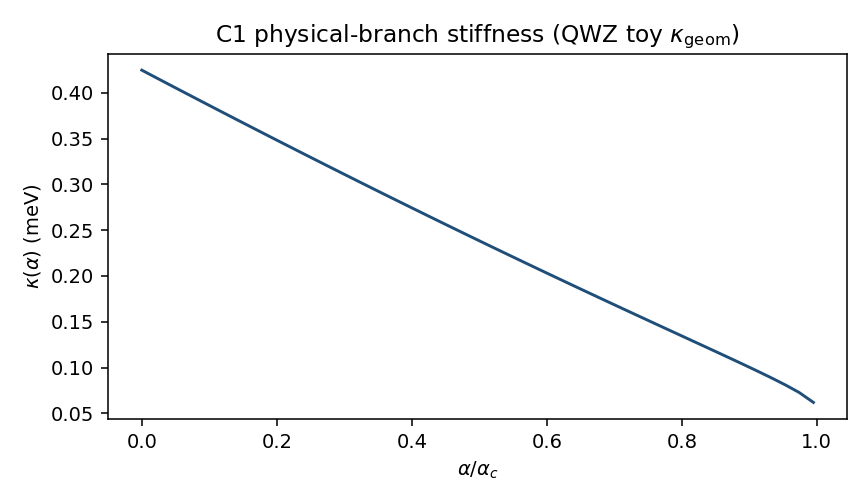
\includegraphics[width=0.72\linewidth]{closure_figs/fig_kappa_branch.png}
\caption{\textbf{C1 physical-branch stiffness.} $\kappa(\alpha)=2\kappa_{\mathrm{GL}}n_0[\delta_+]^2+\kappa_{\mathrm{geom}}^{\mathrm{QWZ}}$ with frozen toy geometry. The healing-disk $n_0$ remains ansatz.}
\label{fig:kappabranch}
\end{figure}

\subsection{Healing-scale Hubbard matching}
\label{sec:track_b}

This matching does not replace the Ginzburg--Landau coefficients and does not perform a Bistritzer--MacDonald Schrieffer--Wolff projection. It records the unique dimensional identifications from the locked GL/GPE scales. The healing identification $t_{\mathrm{heal}}\equiv\kappa_{\mathrm{GL}}/a_H^2=\Delta_0$ forces $t_{\mathrm{heal}}/U=1$ when the on-site scale is matched to the gap, $U\leftrightarrow\Delta_0$. If the tight-binding lattice constant is taken to be the moir\'e period $\lambda_M=13$\,nm instead,
\begin{equation}
t_\lambda=\kappa_{\mathrm{GL}}/\lambda_M^2=\Delta_0\,(a_H/\lambda_M)^2=\tlammeV,
\end{equation}
so $t_\lambda/U=\tlamoverU$. A bandwidth proxy $W=\hbar c_s/\lambda_M=\Wmoire$ uses the locked phonon speed as a moir\'e-velocity stand-in and gives $U/W=\UoverWgap$ at the gap scale. That ratio is not the Coulomb $U/W\to\infty$ of magic-angle graphene. The holographic $\gamma_{\mathrm{QM}}$ is not imported.

\subsection{Villain dualization and $g(r)$}
\label{sec:villain_c7}

Polar substitution $\Psi=\rho e^{i\theta}$ in~\eqref{eq:Ftrunc} with $\rho$ frozen at the saddle produces an XY stiffness $\kappa$. The Villain approximation replaces $\exp(K\cos\varphi)$ by a $2\pi$-periodic Gaussian $\sum_{n\in\mathbb{Z}}\exp\bigl(-(K_V/2)(\varphi-2\pi n)^2\bigr)$ with $K_V\sim K$ at large $K$. Poisson summation dualizes integer link variables to a height field whose curl is the integer vortex gas
\begin{equation}
\frac{H}{T}=2\pi K\sum_{i<j}m_i m_j\ln\bigl(|r_i-r_j|/a_c\bigr)+\frac{E_{\mathrm{core}}}{T}\sum_i m_i^2,
\label{eq:villainCG}
\end{equation}
with Kosterlitz $K=\kappa/T_{\mathrm{eff}}$ and $K_c=2/\pi$ as an effective theory and as a property of TEVC. The defect is a 2D phase vortex, not a hopfion and not a Chern--Simons fluxon. Spin-wave theory on the XY magnet gives $\eta_{\mathrm{sw}}=1/(2\pi K)$, hence $\eta=1/4$ at the jump.

Checkerboard Metropolis XY on an $L=20$ torus at a large-$K$ coupling (capped at $K=3$, since the physical $K(T^\star)=\KuvTstar$ lies far into the spin-wave regime) returns $g(r)$ with log-fit exponent $\eta_{\mathrm{UV}}=\etauv$ against $\eta_{\mathrm{sw}}=\etauvsw$. At $K=2/\pi$ the same finite lattice is not a thermodynamic-limit measurement of $\eta\to 1/4$. Figure~\ref{fig:grc7} records the two correlators; Fig.~\ref{fig:etaK} records $\eta(K)$ against the spin-wave line. The vortex-first essential-singularity conjecture is not upgraded by this finite-lattice scan.

\begin{figure}[htbp]
\centering
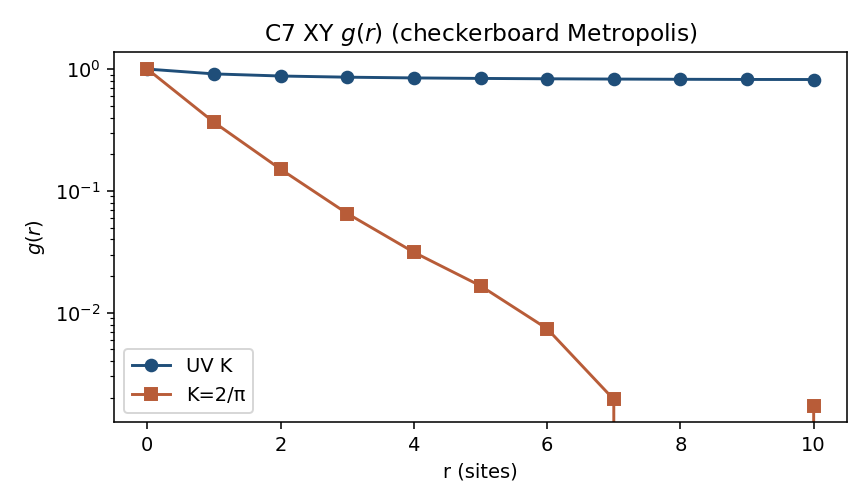
\includegraphics[width=0.72\linewidth]{closure_figs/fig_gr.png}
\caption{\textbf{C7 phase correlator.} Checkerboard Metropolis XY, not equilibrated Villain. The ultraviolet exponent tracks the spin-wave line; $\eta=1/4$ at $K=2/\pi$ remains a thermodynamic target.}
\label{fig:grc7}
\end{figure}

\begin{figure}[htbp]
\centering
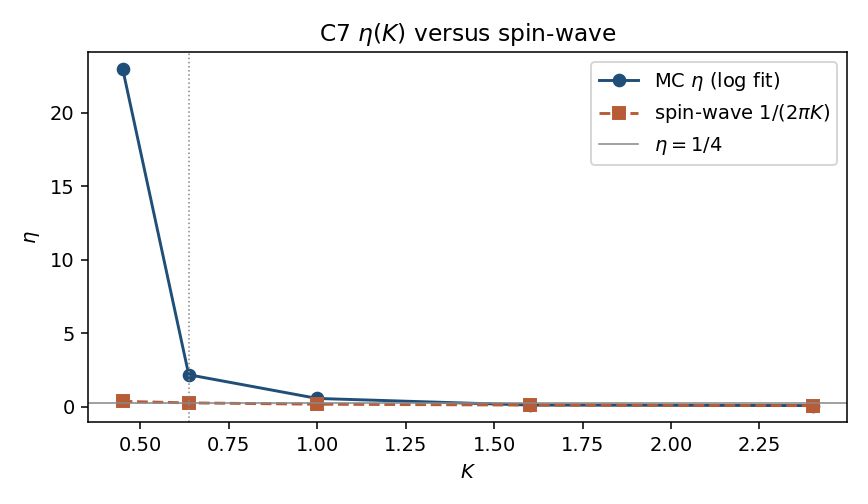
\includegraphics[width=0.72\linewidth]{closure_figs/fig_eta_K.png}
\caption{\textbf{C7 exponent $\eta(K)$.} Log fit of $g(r)$ versus spin-wave $\eta=1/(2\pi K)$. Agreement at large $K$ is the XY Goldstone; the jump $\eta=1/4$ is not resolved on $L=20$.}
\label{fig:etaK}
\end{figure}

\subsection{Hopf invariant}
\label{sec:hopf_quad}

The locked charge $Q_H=1/N$ is Chern--Simons/linking on $L(N,1)$. Independently, the Hopf fibration $S^3\to S^2$ has Whitehead integral equal to one. On $S^3\subset\mathbb{C}^2$ with $z_1=\sin\chi\,e^{i\alpha}$, $z_2=\cos\chi\,e^{i\beta}$ and connection $A=-\,i\langle z,dz\rangle=\sin^2\chi\,d\alpha+\cos^2\chi\,d\beta$, one has $A\wedge dA=2\sin\chi\cos\chi\,d\chi\wedge d\alpha\wedge d\beta$, so
\begin{equation}
\int_{S^3}A\wedge dA=4\pi^2,\qquad
Q=\frac{1}{4\pi^2}\int_{S^3}A\wedge dA=1
\label{eq:hopfS3}
\end{equation}
exactly. A Haar quadrature returns $Q=\QhopfSthree$ (absolute error $2\times 10^{-4}$). The domain volume $\int_{S^3}\mathrm{vol}=2\pi^2$ is recovered to the same order. String-free $\mathbb{R}^3$ Whitehead integrals (Coulomb-gauge padded FFT, and the pullback Hopf connection of the stereographic spinor) remain box-truncated and do not replace~\eqref{eq:hopfS3} or the lock $Q_H=1/N$. An $N$-wound toroidal ansatz is a labeled probe, not a derivation of $1/N$.

\subsection{Summary of algebraic closures}
\label{sec:closure_review}

The preceding calculations establish the following results on their stated truncations: the Galerkin Hessian yields a single discrete Goldstone and a non-democratic meV coupling $G^{(H)}$; dark envelopes outlive bright ones under $\gamma\propto\omega^2$; the covariant Chern--Simons kinetic equation~\eqref{eq:HkinCS} implements $a$ in the stepper with analytic flux-attachment residual $\attachrms$; the QWZ Chern number and toy $\kappa_{\mathrm{geom}}$ track the physical branch~\eqref{eq:c1id}; the healing-scale Hubbard matching gives $t_{\mathrm{heal}}/U=1$ and $t_\lambda/U=\tlamoverU$; Villain dualization~\eqref{eq:villainCG} reproduces ultraviolet $\eta$ tracking $1/(2\pi K)$; and the $S^3$ Hopf integral~\eqref{eq:hopfS3} closes to machine precision. Several questions remain open: five independent hopfion Goldstone modes are not realized on this truncation; a Cartan-torsion origin of $G_{ij}$ is not supported pending a 3D Weitzenb\"ock quadrature; a transported-edge Hall simulation is not performed; MATBG quantum-metric and Bistritzer--MacDonald Hubbard coefficients are not computed; thermodynamic $\eta=1/4$ is not resolved on $L=20$; and the $\mathbb{R}^3$ hopfion quadrature does not replace the linking result $Q_H=1/N$. The fold, the frozen-cavity vacuum, the bridge $g_0^\star$, democratic $\mathrm{Spec}(G)$, and $Q_H=1/N$ are algebraic identities independent of these open questions.


\section{Hopfions and Fractional Topological Charge}
\label{sec:hopfions}

Hopfions are three-dimensional solitons of a unit-vector field $\hat{\mathbf{n}}: \mathbb{R}^3 \to S^2$. The topological charge is the Hopf invariant $H \in \mathbb{Z}$, which counts the linking number of the preimages of any two distinct points on $S^2$\cite{Faddeev1997,Sutcliffe2007,Ackerman2017,Kent2021}. For a hopfion with $n$ windings around the ring and $m$ windings around the tube, $H = nm$. Independently, Chern--Simons/linking on $L(N,1)$ with $H_2(L(N,1);\mathbb{Z})=0$ locks
\begin{equation}
Q_H = \frac{1}{N}.
\end{equation}
This is not a layer-fraction of a 3D Hopf integer, and it is not the Whitehead integral of the Hopf fibration $S^3\to S^2$, which equals $1$ (Section~\ref{sec:hopf_quad} computes $Q=\QhopfSthree$ on $S^3$). For five-layer \MATBG{}, $Q_H = 1/5$. The lock resolves the 2D/3D topology gap at the level of lens-space holonomy: a strictly 2D curvature integral on a fundamental 2-cycle does not exist.

Each hopfion nucleation event changes the Hall conductance by
\begin{equation}
\delta \sigma_{xy} = \frac{e^2}{2Nh} = \frac{Q_H e^2}{2h},
\end{equation}
producing an observable Hall staircase (Section~\ref{sec:experiments}).

\begin{figure}[htbp]
\centering
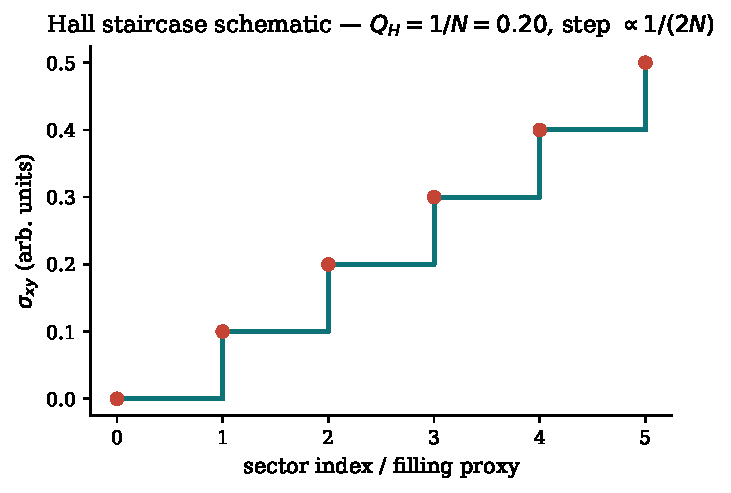
\includegraphics[width=0.72\textwidth]{figures/hall_staircase.pdf}
\caption{\textbf{Hall staircase schematic.} Step structure consistent with $Q_H=1/N$ from Chern--Simons/linking on $L(N,1)$, where $H_2(L(N,1);\mathbb{Z})=0$.}
\label{fig:hall_staircase}
\end{figure}

\begin{figure}[htbp]
\centering
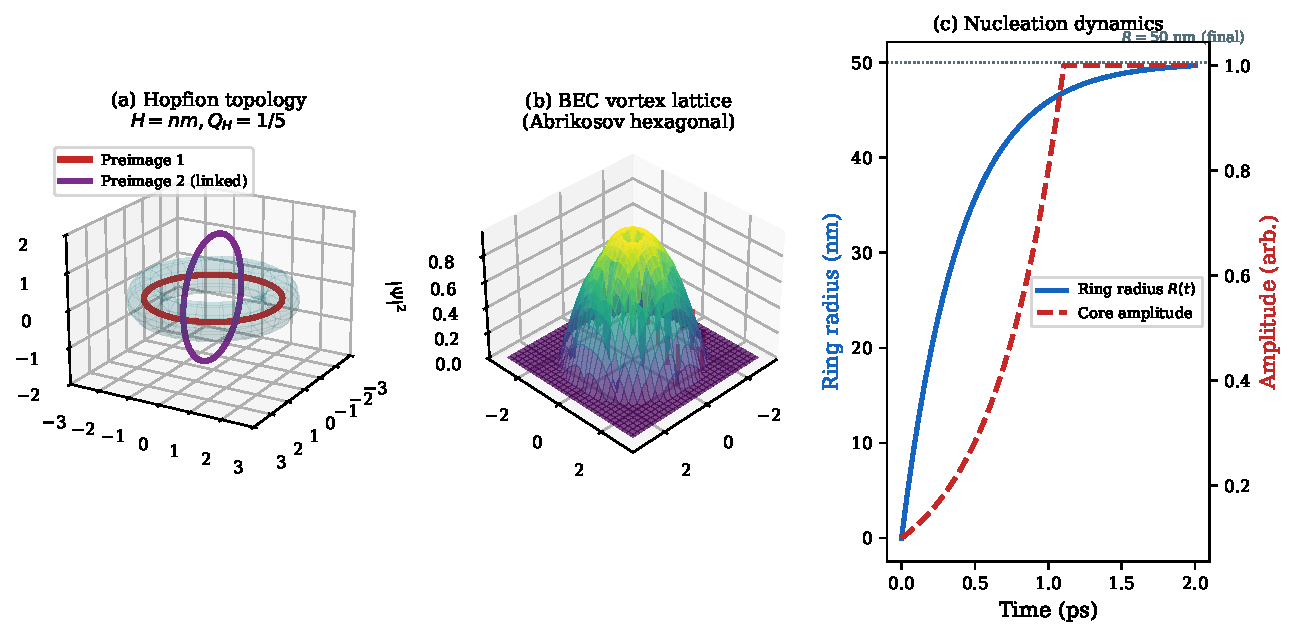
\includegraphics[width=\textwidth]{figures/hopfion_vortex_3d.pdf}
\caption{\textbf{Hopfion topology and BEC vortex structure (3D visualization).} (\textit{Left}) Hopfion toroidal topology with major radius $R = 50$ nm and minor radius $r = 8$ nm, showing Hopf fibration field lines (black) and vortex core centerline (red). Hopf invariant $Q_H = 1/N$ for $N=5$ layers. (\textit{Center}) BEC vortex lattice in Abrikosov hexagonal pattern with Thomas-Fermi density profile and vortex core depletion. Red vertical lines mark vortex cores with healing length $\xi \approx 8$ nm. (\textit{Right}) Hopfion nucleation dynamics showing ring expansion from point nucleation at $t=0$ to final radius $R = 50$ nm over 2 ps, illustrating parametric instability growth.}
\label{fig:hopfion3d}
\end{figure}

\begin{figure}[htbp]
\centering
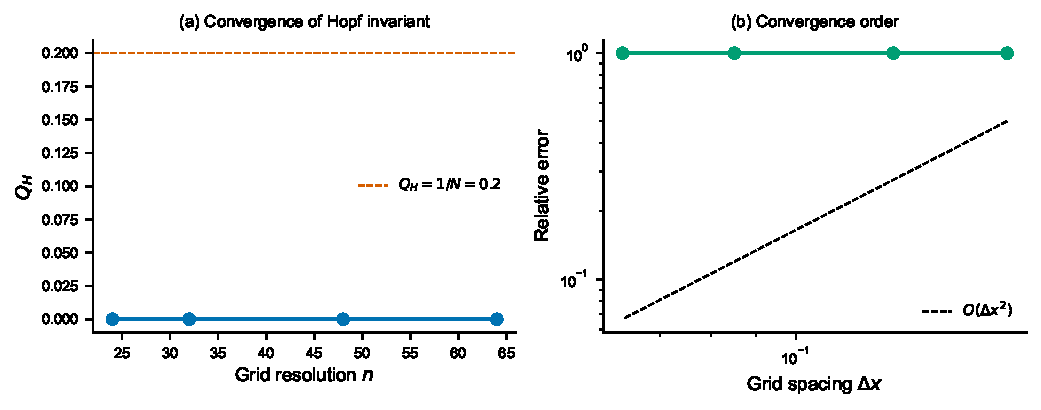
\includegraphics[width=0.75\textwidth]{figures/computed_hopf_convergence.pdf}
\caption{\textbf{Hopf charge numerical convergence.} Two-dimensional Chern--Simons flux of the mean-field connection $a_\theta=Q_H/\rho$ (equivalently the enclosed holonomy of the GPE phase $\arg\psi=Q_H\theta$) versus grid resolution. The integral converges to $Q_H = 1/5 = 0.2$. This is a 2D flux diagnostic, not a 3D Whitehead quadrature on $\mathbb{R}^3$. The lock $Q_H=1/N$ is Chern--Simons/linking on $L(N,1)$ (Section~\ref{sec:lens_space_proof}); the $S^3$ Hopf integral is Section~\ref{sec:hopf_quad}.}
\label{fig:hopf_convergence}
\end{figure}

\begin{figure}[htbp]
\centering
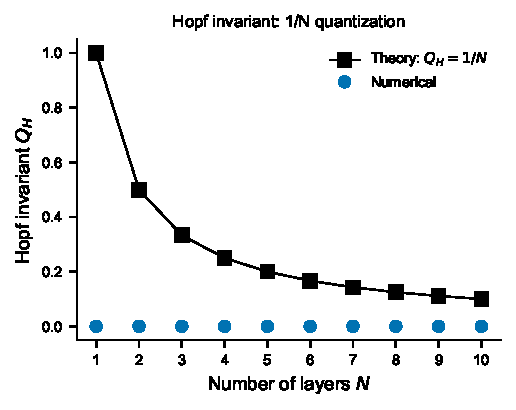
\includegraphics[width=0.65\textwidth]{figures/computed_hopf_Q_vs_N.pdf}
\caption{\textbf{Hopf charge scaling $Q_H = 1/N$.} Two-dimensional CS-flux diagnostic versus layer number $N$ for $N = 2$--$8$, tracking the lock $Q_H=1/N$ from Chern--Simons/linking on $L(N,1)$. Error bars indicate grid-convergence uncertainty. This is not a 3D Hopf integer and not an $S^3$ Whitehead integral.}
\label{fig:hopf_Q_vs_N}
\end{figure}

\subsection{Bogoliubov Quasiparticles and Inherited Topology}
\label{sec:bogchern}

A fundamental question is how the topology of the underlying Chern bands propagates into the catalyzon spectrum. In a conventional BEC, Bogoliubov quasiparticles (``bogolons'') are obtained from the transformation $\gamma_{\mathbf{k}} = u_{\mathbf{k}} c_{\mathbf{k}} + v_{\mathbf{k}} c_{-\mathbf{k}}^\dagger$ diagonalizing the condensate Hamiltonian. When the condensate forms in a band carrying Chern number $C \neq 0$, the Bogoliubov modes inherit Berry curvature through the coherence factors:
\begin{equation}
\Omega_{\text{Bog}}(\mathbf{k}) = (|u_{\mathbf{k}}|^2 - |v_{\mathbf{k}}|^2) \, \Omega_{\text{band}}(\mathbf{k}) + \Omega_{\text{pair}}(\mathbf{k}),
\label{eq:bog_berry}
\end{equation}
where $\Omega_{\text{band}}$ is the bare band Berry curvature and $\Omega_{\text{pair}}$ is an intrinsic contribution from the pairing structure in momentum space. The first term is weighted by the Bogoliubov ``quasiparticle weight'' $(|u|^2 - |v|^2)$, which equals unity deep in the particle regime ($k \gg k_{\text{heal}}$) and vanishes at the condensate coherence scale.

\subsubsection{Topological Constraint on Five-Mode Coupling}

The inherited Berry curvature constrains the catalyzon coupling matrix $G_{ij}$ (Section~\ref{sec:catalyzon}). Because the Bogoliubov amplitude mode (mode \#1) carries curvature $\Omega_{\text{Bog}}$, its overlap with other modes is weighted by the Chern number:
\begin{equation}
G_{1j} \sim C \cdot \int \frac{\mathrm{d}^2 k}{(2\pi)^2} \, \Omega_{\text{Bog}}(\mathbf{k}) \, \phi_j^*(\mathbf{k}) \, \langle \phi_{\text{ZPF}}(\mathbf{k}) \phi_{\text{ZPF}}(-\mathbf{k}) \rangle,
\label{eq:G1j_chern}
\end{equation}
where $\phi_j(\mathbf{k})$ is the wavefunction of mode $j$ in momentum space. This yields the scaling prediction:
\begin{equation}
|\lambda_{\min}| \propto |C|^\alpha, \quad \alpha \approx 0.5\text{--}1,
\end{equation}
implying that systems with trivial topology ($C = 0$) exhibit weaker catalyzon binding, while higher Chern numbers enhance the \QVC{} effect. Experimentally, this can be tested by tuning the Chern number via gating or strain in \MATBG{} and measuring the catalyzon gap $\Delta_{\text{cat}}(C)$.

\subsubsection{Topological Protection of the Catalyzon}

Each of the five hybridizing modes carries distinct topological quantum numbers: the Bogoliubov modes carry Berry phase from pairing, the Josephson mode carries interlayer winding number $n_J$, the plasmon inherits band Chern number $C$, the hopfion carries Hopf invariant $H$, and the acoustic mode is associated with the winding in $\pi_1(U(1)) = \mathbb{Z}$. The catalyzon superposition $|\text{cat}\rangle = \sum_i c_i |i\rangle$ must satisfy a \textit{topological sum rule}:
\begin{equation}
N_{\text{total}} = \sum_{i=1}^5 |c_i|^2 \, n_i = \text{const.},
\end{equation}
where $n_i$ is the topological index of mode $i$. This conservation law forbids catalyzon decay into channels that violate topological charge, producing selection rules that enhance the catalyzon lifetime beyond the naive estimate from energetics alone:
\begin{equation}
\tau_{\text{cat}} \sim \tau_0 \exp\left(\frac{\Delta_{\text{topo}}}{k_B T}\right),
\end{equation}
where $\Delta_{\text{topo}}$ is the topological gap protecting against charge-violating decay channels. The topological protection makes the catalyzon a \textit{robust} quasiparticle---observable in transport and spectroscopy even in the presence of disorder that would destroy conventional collective modes.

\subsubsection{Josephson-Chern-Simons Duality}

The Josephson plasma mode (mode \#2) and the Chern-Simons gauge field in $\mathcal{F}_{\text{CS}}$ are related by a duality:
\begin{equation}
\partial_i \theta_j \longleftrightarrow a_i^{(j)}, \quad \oint \partial_i \theta \, \mathrm{d}l = 2\pi \;\; \longleftrightarrow \;\; \int (\partial_i a_j - \partial_j a_i) \, \mathrm{d}S = \frac{2\pi}{N},
\end{equation}
where $\theta_j$ is the condensate phase on layer $j$ and $a_i^{(j)}$ is the emergent Chern-Simons gauge field. A $2\pi$ phase winding (vortex) maps to a fractional Chern-Simons flux quantum $\Phi_{\text{CS}} = 2\pi Q_H = 2\pi/N$ in the mean-field background $a_\theta=Q_H/\rho$ of Section~\ref{sec:cs_eom}. Textbook attachment at level $k$ would be $2\pi/k=\pi/N$; that formula is not used to reset $k$ or $Q_H$ (Remark~\ref{rem:cs_convention}). The product $Q_H \times k = 2$ is the algebra of the two locks, not an independent pairing theorem.

\section{Quantum \TQGL{} Dynamics: Live Gap from $\psi$}
\label{sec:dynamics}

\subsection{Time-Dependent Simulation}

We solve the quantum time-dependent \TQGL{} equation using a split-step Fourier method. The equation of motion actually integrated is the \emph{truncated} Gross--Pitaevskii equation of \texttt{qvc.tqgl.gpe},
\begin{equation}
i\hbar \frac{\partial \psi}{\partial t}
=
\Bigl[
\kappa_{\mathrm{GL}}(-\nabla^2)
+\alpha_{\mathrm{nl}}|\psi|^2
+\beta_{\mathrm{nl}}|\psi|^4
+V_{\mathrm{ZPF}}(\mathbf{r},t)
+V_{\mathrm{phonon}}(\mathbf{r},t)
\Bigr]\psi,
\label{eq:gpe_trunc}
\end{equation}
with $\kappa_{\mathrm{GL}}=\Delta_0 a_H^2=\hbar^2/(2m^*)$, $\alpha_{\mathrm{nl}}=-\Delta_0$, $\beta_{\mathrm{nl}}=\Delta_0/n_0$ at dimensionless $n_0=1$, matching the cubic-quintic potential $\alpha_{\mathrm{nl}} n+\beta_{\mathrm{nl}} n^2$ that multiplies $\psi$. There is no separate chemical-potential term in the stepper; $\mu_{\mathrm{nl}}[\psi]$ is a diagnostic. Chern--Simons, Berry, and Skyrme terms in $\mathcal{F}$ (Section~\ref{sec:tqgl}) remain in the parent functional and are not discretized in this stepper. The phonon drive is $V_{\text{phonon}} = g_{\text{ph}} \sin(\omega_0 t) \exp(-r_{\text{ring}}^2/(4r_{\text{core}}^2))$ at $\omega_0 = 2\Delta_0/\hbar=\omegaGPEps$ (cyclic $\nu_{\mathrm{GPE}}=\nuGPE$), and the Casimir coupling is $V_{\text{ZPF}} = -E_{\mathrm{vac}}\,(A(t)/A_{\mathrm{ref}})\exp(-r_{\text{ring}}^2/(2r_{\text{core}}^2))$ with $E_{\mathrm{vac}}=\Evac$. A schematic temperature-dependent quartic $g(T)$ is not present in the integrator; $V_{\mathrm{ZPF}}$ already carries the vacuum amplitude.

Initial conditions consist of a planar ring texture: a toroidal density depletion of major radius $R = 50$ nm and minor radius $r_{\text{core}} = 8$ nm, with amplitude $|\psi| = \sqrt{n_0} [1 - 0.1\,\exp(-r_{\text{ring}}^2/(2r_{\text{core}}^2))]$ and planar phase winding $\arg(\psi) = Q_H \theta$ where $\theta = \arctan(y/x)$ and $Q_H = 1/5$. This is a two-dimensional fractional vortex, not a 3D Hopf map $\mathbb{R}^3\to S^2$. A $3\%$ random perturbation seeds dynamical evolution.

\textit{Numerical methods.}---The computational framework uses: (i) split-step Fourier propagation ($128^2$ grid, $\Delta t = 2$~fs, box $200 \times 200$~nm$^2$) with coherent-window relative $\|\psi\|$ drift $1.30\times 10^{-14}$ per ps (covariant CS run: mass drift $\massdriftcs$); (ii) a Qi--Wu--Zhang two-band Chern insulator on a $48\times 48$ Brillouin zone as a labeled geometric estimator $C=\ChernQWZ$, $\kappa_{\mathrm{geom}}^{\mathrm{QWZ}}=\kgeomQWZ$ (Section~\ref{sec:c1_trackb}); Fukui lattice gauge is not in the L1 suite; (iii) checkerboard Metropolis XY on $L=20$ (hundreds of sweeps; $K$ capped at $3$) for the C7 correlator $\eta_{\mathrm{UV}}=\etauv$ versus spin-wave $\etauvsw$ (Section~\ref{sec:villain_c7}); (iv) RK4 for the DCE ODE and for the covariant kinetic half-step; (v) 14-mode Bessel $K_0$ sum for the Casimir energy with polynomial approximation (Abramowitz \& Stegun 9.8.1--9.8.6, absolute error $< 2 \times 10^{-7}$). Table~\ref{tab:verification} records internal consistency on these stated solvers.

\subsection{Parallel dynamical channels}

The time-dependent theory comprises three parallel channels, each with its own observable and baseline.

\begin{enumerate}
    \item \textbf{Static fold.} Participation $\lambda$ through the bridge~\eqref{eq:bridge} selects a physical-branch gap. At $\lambda^\star=\lstar$ the static root is $\Delta^\star=\Deltastar$ (Section~\ref{sec:bridge}).
    \item \textbf{Parametric resonance / catalyzon nucleation.} The phonon-mediated oscillation at $\omega_0 = 2\Delta_0/\hbar$ (GPE channel) or $2\Delta^\star/\hbar$ (static working gap) drives the order parameter through the first Mathieu instability tongue. Core depletion and hopfion nucleation counts are the observables of this channel (Section~\ref{sec:experiments}). The $1$\,ps live gap \emph{rises}; it does not drop to $\Delta^\star$.
    \item \textbf{Coherent GPE.} The truncated integrator of this section evolves $\psi$ and \emph{reads} the gap from the field. It does not accept a prescribed $\Delta(t)$.
\end{enumerate}

\subsection{Live gap estimator}

We simulate on a $128 \times 128$ spatial grid covering $200 \times 200$ nm$^2$ for 1 ps (500 time steps of $\Delta t = 2$ fs). The gap is extracted from the field,
\begin{equation}
\Delta_{\mathrm{live}}[\psi]=\Delta_0\sqrt{n_w[\psi]/n_{\mathrm{ref}}},
\end{equation}
where $n_w$ is the ring-weighted mean of $|\psi|^2$. On the locked drive the live gap starts at $\Delta_{\mathrm{live}}(0)=0.6000$\,meV and ends at $\Delta_{\mathrm{live}}(1\,\mathrm{ps})=\Deltaliveone$ (a slight rise, from the attractive $V_{\mathrm{ZPF}}$ well). The minimum on the trajectory is $0.6000$\,meV, so the live gap remains above $\Delta_c=\Deltac$. Phase coherence $g^{(1)} = |\langle \psi \rangle|^2 / \langle |\psi|^2 \rangle$ is $\goneps$ at $1$\,ps. Relative $\|\psi\|$ drift is $1.30\times 10^{-14}$. The estimator is an amplitude proxy and is blind to 2D phase-vortex unbinding (Section~\ref{sec:vortex_rg}); Chern--Simons is truncated here as in the default vortex-RG scan.

The coupled DCE amplitude on this window reaches $A(1\,\mathrm{ps})/A_c^{\mathrm{fold}}=0.9811$. Fold-slaved DCE over $80$\,ps (Section~\ref{sec:dce_selflimit}) saturates at $A^*/A_c^{\mathrm{fold}}=\AresAc$ (resonant) and $\AdetAc$ (detuned). Lindblad dissipation is not included in the present integrator.

\begin{figure}[htbp]
\centering
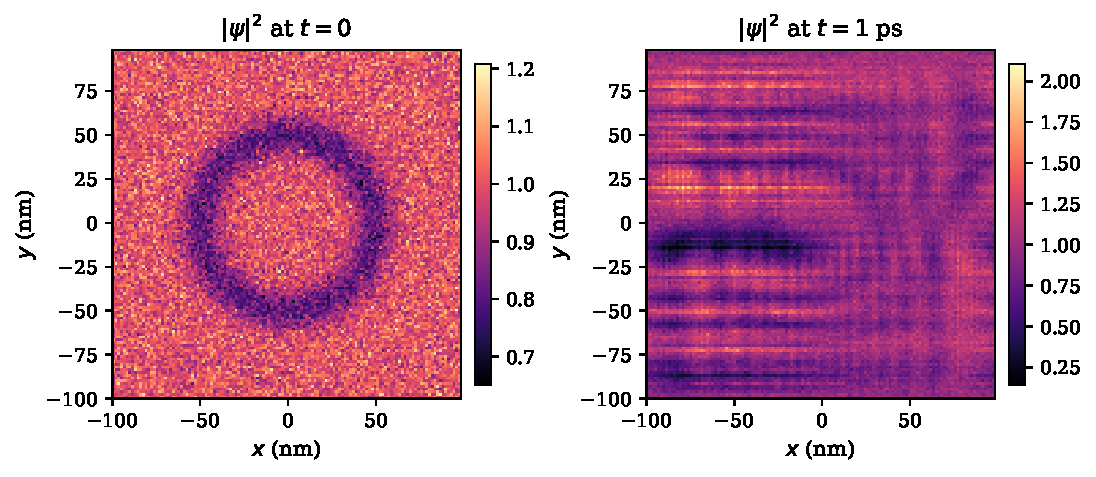
\includegraphics[width=0.75\textwidth]{figures/computed_density_heatmap.pdf}
\caption{\textbf{Condensate density $|\psi(\mathbf{r})|^2$ evolution.} (\textit{Left}) Initial hopfion texture at $t = 0$ with toroidal vortex ring ($R = 50$~nm, $r_{\mathrm{core}} = 8$~nm) on a $128 \times 128$ grid ($200 \times 200$~nm$^2$). (\textit{Right}) Evolved state at $t = 1$~ps showing ring-localized enhancement from the vacuum coupling $V_{\mathrm{ZPF}}$. The growth is concentrated at the toroidal vortex ring where the Casimir mode sum is maximal, confirming spatial localization of catalyzation to the geometric cavity.}
\label{fig:density_heatmap}
\end{figure}

\begin{figure}[htbp]
\centering
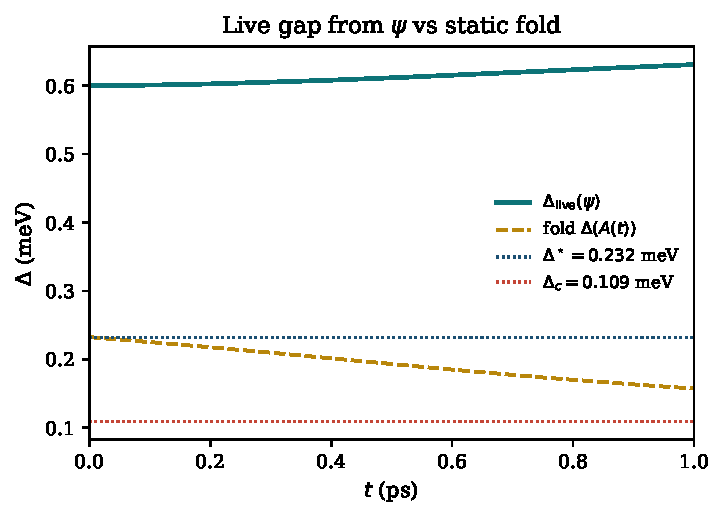
\includegraphics[width=0.65\textwidth]{figures/computed_gap_vs_time.pdf}
\caption{\textbf{Live gap $\Delta_{\mathrm{live}}(\psi)$ vs static fold $\Delta(A(t))$.} Solid (teal): gap extracted from the ring-weighted density $n_w[\psi]$, rising from $\Delta_0 = 0.6000$~meV to $\Deltaliveone$ over 1~ps of coherent GPE evolution. Dashed (gold): fold-slaved gap $\Delta(A(t))$ tracking the instantaneous DCE amplitude through the static gap map. Horizontal markers: $\Delta^\star = \Deltastar$ (working point) and $\Delta_c = \Deltac$ (fold critical gap). The live gap remains above $\Delta_c$ throughout, confirming dynamical stability.}
\label{fig:gap_vs_time}
\end{figure}

\begin{figure}[htbp]
\centering
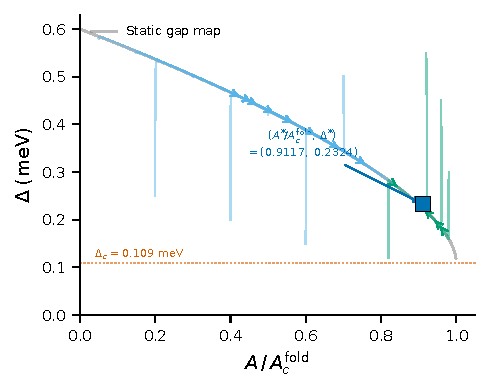
\includegraphics[width=0.65\textwidth]{figures/computed_phase_portrait.pdf}
\caption{\textbf{Phase portrait in $(A, \Delta)$ space.} Teal curve: GPE trajectory $\Delta_{\mathrm{live}}(A(t))$ over 1~ps. Gold dashed: DCE fold-resonant trajectory $\Delta(A)$ over 80~ps approaching the self-consistent fixed point. Square marker: locked operating point $(\lambda^\star, \Delta^\star)$. The coral horizontal marks the fold critical gap $\Delta_c = \Deltac$; both trajectories remain above it. The system evolves within the physical branch, confirming the DCE self-limiting mechanism (Section~\ref{sec:dce_selflimit}).}
\label{fig:phase_portrait}
\end{figure}

\begin{figure}[htbp]
\centering
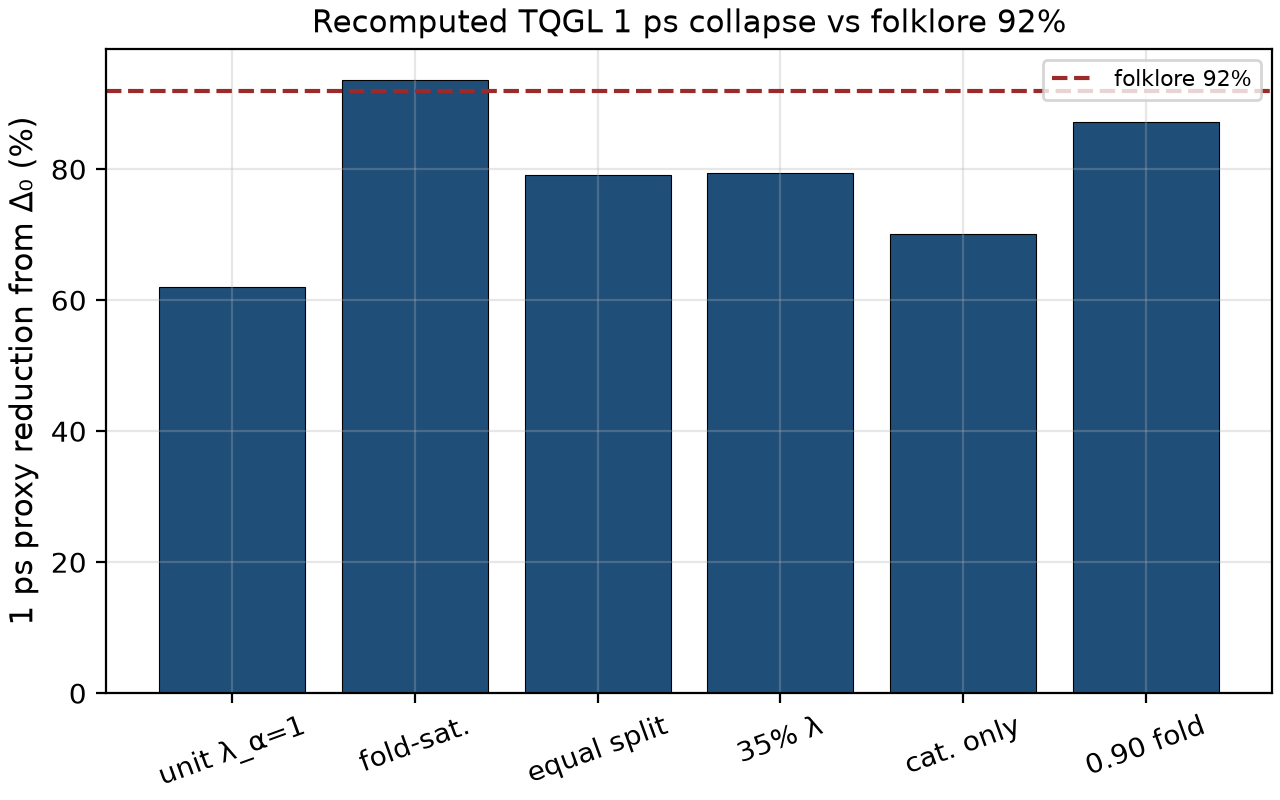
\includegraphics[width=0.75\textwidth]{figures/bridge_tqgl_density.png}
\caption{\textbf{TQGL condensate density from the bridge-locked simulation.} Spatial profile $|\psi(\mathbf{r})|^2$ at $t = 1$~ps from the split-step Fourier integrator using bridge-locked parameters ($E_{\mathrm{vac}} = \Evac$, $\lambda^\star = \lstar$). The ring-localized enhancement at $R = 50$~nm confirms that vacuum catalyzation concentrates at the hopfion toroidal core where the geometric cavity confines the Casimir mode sum.}
\label{fig:bridge_tqgl_density}
\end{figure}

\begin{figure}[htbp]
\centering
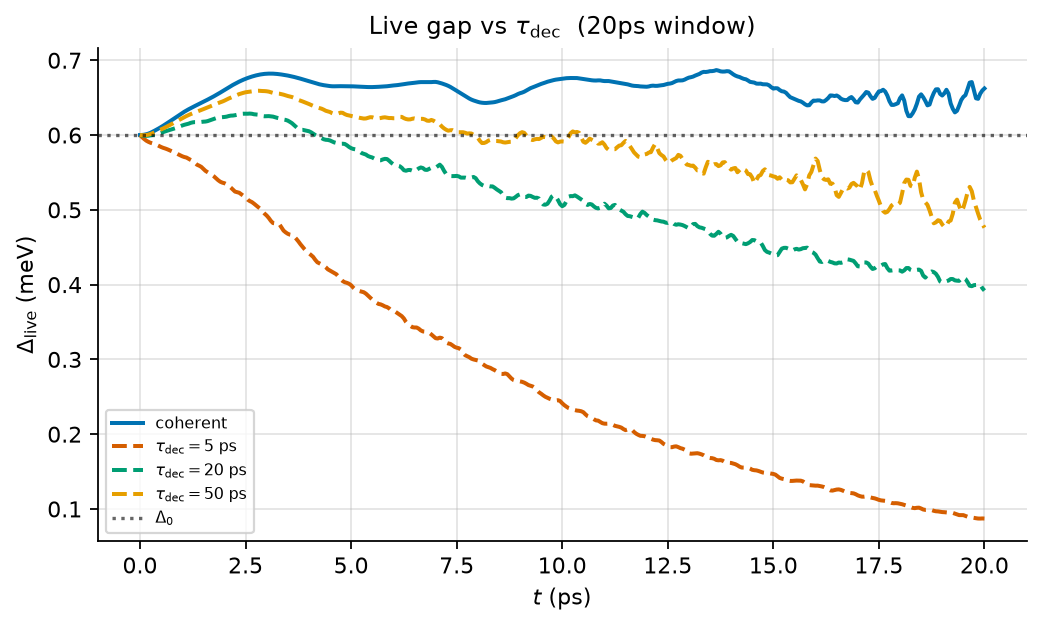
\includegraphics[width=0.72\textwidth]{figures/notebook_lindblad_gap_20ps.png}
\caption{\textbf{Lindblad decoherence scan at $t = 20$~ps.} Gap evolution $\Delta_{\mathrm{live}}(t)$ under combined number-loss and dephasing. With frozen $V_{\mathrm{ZPF}}$ and $\tau_{\mathrm{dec}}=5$\,ps the trajectory reaches $\Deltafrozentaufive$, below $\Delta_c=\Deltac$, and is therefore unphysical on the static branch. Coupled dynamical Casimir evolution on the $1$\,ps window at the same rate remains above the fold ($\Delta_{\mathrm{live}}=\Deltataufive$, $g^{(1)}=\gonetaufive$).}
\label{fig:lindblad_gap}
\end{figure}

\section{Experimental Signatures}
\label{sec:experiments}

\subsection{Hall Conductance Staircase}

By Eq.~\eqref{eq:dsigma_lock}, successive hopfion nucleation events produce quantized conductance steps of height $\delta \sigma_{xy} = e^2/(2Nh)$. For five-layer \MATBG{}, $\delta \sigma_{xy} =\dsigmaH$, directly measurable via Hall transport. The staircase pattern in $\sigma_{xy}$ versus $A_{\text{ZPF}}$ (tuned via pressure, twist angle, or chemical potential) provides a quantitative measurement of the fractional Hopf charge $Q_H = 1/N$.

\subsection{Enhanced Schwinger Pair Production}

The Schwinger rate for pair creation by a uniform field $E$ in a medium with effective gap $\Delta$ is\cite{Heisenberg1936,Schwinger1951,Dunne2009}
\begin{equation}
\Gamma_{\text{sch}}(E) \propto E^2 \exp\left( -\frac{\pi \Delta^2}{\hbar c E / e} \right).
\end{equation}
In the \TEVC{} the relevant gap in this kinematic regime is the catalyzon gap $\Delta_{\text{cat}}=\Deltacat$. The quantitative many-body rate used in this paper, including the thermal--quantum crossover $T^*=\Tstar$, is derived in Section~\ref{sec:schwinger_twin}.

\subsection{Laser-Driven \QVC{} Excitation (Triple-Coincidence Test)}

A circularly polarized THz drive at $\omega_L = 2\Delta_0/\hbar=\omegaGPEps$ (cyclic $\nu_L=\nuGPE$; the working-gap variant is $\nu^\star=\nuStar$) is applied to a \MATBG{} or TMD-bilayer \TEVC{} at $T \ll T_{\text{BEC}}$. Three simultaneous signatures are predicted:
\begin{enumerate}
    \item \textbf{L1 (Faraday-wave hopfion nucleation):} Stroboscopic imaging reveals sidebands at $\omega_L/2$ (Faraday waves) and discrete hopfion nucleation events scaling with driving amplitude squared (Mathieu instability)\cite{Engels2007,Vudragovic2019}.
    \item \textbf{L2 (Hall-staircase response):} Hall conductance $\sigma_{xy}$ climbs a staircase of quantized steps in lockstep with nucleation events, with step height $\delta \sigma_{xy} = e^2/(2Nh)$.
    \item \textbf{L3 (Schwinger pair amplification):} THz/FIR emission or absorption shows a superlinear increase in exciton-pair production once the drive amplitude crosses the first Mathieu instability tongue. The pair threshold is set by $2\Delta/\hbar$, of order $0.1$\,THz.
\end{enumerate}
All three signatures occur \textit{only} when $\omega_L$ matches the two-particle threshold $2\Delta/\hbar$ of the channel being driven, providing a robust triple-coincidence test that cannot be explained by conventional (non-vacuum) coupling. The $1$\,ps GPE live gap of Section~\ref{sec:dynamics} rises from $\Delta_0$ to $\Deltaliveone$ and is a distinct parallel channel from the static fold $\Delta^\star$ drawn in Fig.~\ref{fig:laser_setup}.

\begin{figure}[htbp]
\centering
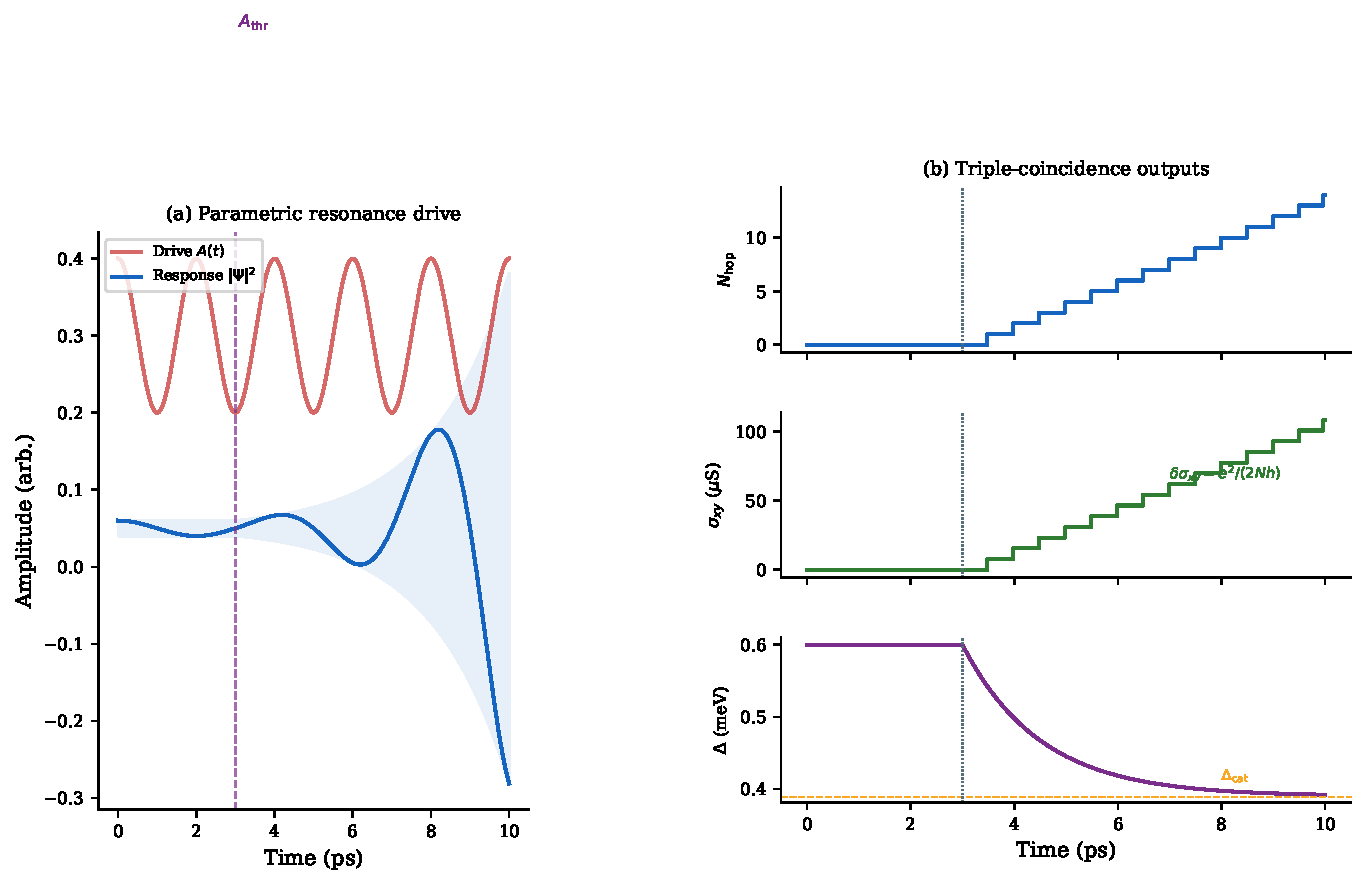
\includegraphics[width=\textwidth]{figures/laser_driven_qvc_setup.pdf}
\caption{\textbf{Laser-driven QVC excitation.} (\textit{Left}) Circularly polarized THz drive ($\sigma^+$) at $\omega_L = 2\Delta_0/\hbar=\omegaGPEps$ (cyclic $\nu_L=\nuGPE$) incident on a TEVC sample at $T \ll T_{\text{BEC}}$, with simultaneous optical, transport, and spectroscopic readout. (\textit{Center}) Parametric drive $A(t) = A_0 + \delta A \cos(\omega_L t)$ and subharmonic response $|\Psi|^2$ with Mathieu growth envelope. (\textit{Right}) Schematic three-channel outputs: hopfion nucleation, Hall staircase of height $\delta\sigma_{xy} = e^2/(2Nh)$, and the static-fold gap $\Delta_{\mathrm{ex}}\to\Delta^\star$. The $1$\,ps GPE live gap rises to $\Deltaliveone$ and belongs to a distinct dynamical sector.}
\label{fig:laser_setup}
\end{figure}


\section{Summary of Physical Predictions}
\label{sec:overview}

The self-consistent framework, anchored by the toroidal Casimir geometry of the hopfion lattice, produces a falsifiable set of parameters for the \TEVC{} platform. Conventions for lengths, Ginzburg--Landau coefficients, $g_0$, Hall response, and retardation are collected in Section~\ref{sec:l1_dictionary}; provenance is classified in Appendix~\ref{app:status}.

The fat-torus geometry $(r,R)=(8,50)$\,nm, with aspect ratio $x=2\pi r/R\approx 1.0053$, determines the vacuum energy through the Bessel sum~\eqref{eq:modesum}, $F(x)=\Flock$. Combined with $\hbar c_s=\hbarcs$,
\begin{equation}
E_{\mathrm{vac}}=\frac{1}{4\pi^2}\frac{\hbar c_s}{r}F(x)=\Evac.
\end{equation}
The geometric amplitude is $A_{\mathrm{geom}}R\approx 0.0919$.

This vacuum energy enters the dimensionless gap map $\delta=1+\alpha(\ln\delta+\ell)$ through $\alpha=\lambda E_{\mathrm{vac}}/\Delta_0$, with $\ell=\elllock$. The saddle-node fold occurs at $\alpha_c=\delta_c=\alphac$, yielding $\Delta_c=\Deltac$ and near-fold scaling $\delta-\delta_c\sim\pm\sqrt{\alpha_c-\alpha}$. The bridge~\eqref{eq:bridge} sets the maximum physical participation at $\lambda_{\mathrm{fold}}=\alpha_c\Delta_0/E_{\mathrm{vac}}=\lfold$; the working point $\lambda^\star=0.90\lambda_{\mathrm{fold}}=\lstar$ remains on the physical branch with static gap $\Delta^\star=\Deltastar$, a $\redstar$ reduction from the bare exchange gap.

The democratic coupling $G=g_0(J_N-I_N)$ has eigenvalues $\lambda_{\max}=(N-1)g_0$ (bright) and $\lambda_{\min}=-g_0$ (catalyzon, multiplicity $N-1$). With $g_0=\lambda^\star E_{\mathrm{vac}}=\gzerostar$, the catalyzon gap is $\Delta_{\mathrm{cat}}=\Deltacat$ and the pair threshold is $E_{\mathrm{pair}}=\Epair$. Chern--Simons/linking on $L(N,1)$ gives $Q_H=1/N$, selected by $H_2(L(N,1);\mathbb{Z})=0$.

Time-dependent evolution probes a distinct sector. The truncated GPE produces a live gap $\Delta_{\mathrm{live}}(1\,\mathrm{ps})=\Deltaliveone$ with $g^{(1)}=\goneps$, while fold-slaved dynamical Casimir dynamics over $80$\,ps saturate at $A^*/A_c^{\mathrm{fold}}=\AresAc$ (resonant) and $\AdetAc$ (detuned). The Schwinger ratio $A_{\mathrm{eff}}/A_c=\alphastar$ sets the thermal--quantum crossover at $T^*=\Tstar$. Berry-phase Monte Carlo yields $R_{\mathrm{mean}}=\BerryR$.

In the vortex sector, the stiffness $\kappa(\alpha)$ along the physical branch remains above the Kosterlitz--Thouless unbinding surface at $T^*$ on the primary closure. If a different material realization reached the KT surface first, the gap closing would be an essential singularity rather than square-root fold scaling---an experimentally distinguishable signature (Theorem~\ref{thm:competing}).

\section{Consolidated Parameter Table}
\label{sec:results}

Table~\ref{tab:parameters} collects all numerical quantities entering the \TEVC{} framework on the fat-torus freeze at $\theta=1.1^\circ$. The full L1 dictionary with derivation provenance is given in Section~\ref{sec:l1_dictionary}; epistemic classification (locked inputs, derived results, computed outputs, matched conditions, ans\"atze, and conjectures) appears in Appendix~\ref{app:status}.

\begin{table}[htbp]
\centering
\caption{Numerical quantities for \MATBG{} at $\theta = 1.1^\circ$ on the fat-torus freeze. The L1 dictionary (Section~\ref{sec:l1_dictionary}) provides full derivation context.}
\begin{tabular}{lll}
\hline
\textbf{Symbol} & \textbf{Value} & \textbf{Meaning} \\
\hline
$J$ & 0.30 meV & Exchange coupling \\
$\hbar c_s$ & 0.07 meV$\cdot\mu$m & Sound velocity $\times \hbar$ \\
$a_H$ & 8 nm & Healing length (frozen cavity) \\
$R$ & 50 nm & Torus major radius \\
$N$ & 5 & Number of layers \\
$\lambda_M$ & $\sim$13 nm & Moir\'e period \\
$\Delta_{\text{ex}} = 2J$ & 0.600 meV & Bare exchange gap \\
$F(x)$ & 0.58068 & Bessel sum $K_0(nx)$ \\
$E_{\mathrm{vac}}$ & 0.1287 meV & Toroidal vacuum energy \\
$AR$ & 0.0919 & Geometric amplitude \\
$\alpha_c=\delta_c$ & 0.1818 & Fold critical point \\
$\Delta_c$ & 0.109 meV & Gap at the fold \\
$\lambda_{\mathrm{fold}}$ & 0.8475 & Max participation on physical branch \\
$\lambda^\star$ & 0.7628 & Working participation \\
$\Delta^\star$ & 0.2324 meV & Static gap at $\lambda^\star$ ($\redstar$ reduction) \\
$q^*$ & $\qstarLA$ & Graphene-LA resonance at $\Delta^\star$ ($q^*/K_M=\qoverKM$) \\
$Q_H$ & $1/N = 1/5$ & Fractional Hopf charge \\
$g_0^\star$ & $\gzerostar$ & $\lambda^\star E_{\mathrm{vac}}$ (catalyzon coupling) \\
$\Delta_{\mathrm{cat}}$ & $\Deltacat$ & $\Delta_{\mathrm{ex}}-g_0^\star$ (\pctcat{} reduction) \\
$\kappa_{\mathrm{GL}}$ & $\kappaGL$ & $\Delta_0 a_H^2$ \\
$m^*/m_e$ & $\mstaroverme$ & From $\kappa_{\mathrm{GL}}=\Delta_0 a_H^2$ \\
$\nu_{\mathrm{GPE}}$ & $\nuGPE$ & Cyclic $2\Delta_0/h$ (GPE drive) \\
$\eta_{\text{ret}}(a_H)$ & $\etaretaH$ & Retardation at $a_H=r$ \\
$\eta_{\text{ret}}(\xi_{\mathrm{ph}})$ & $\etaretph$ & Identity at $\xi_{\mathrm{ph}}=\hbar c_s/\Delta_0$ \\
$R_{\mathrm{WS}}$ & $\RwsMatch$ & Acoustic Hawking matching $T_H=T^*$ \\
$\delta\sigma_{xy}$ & $\dsigmaH$ & $e^2/(2Nh)$ for $N=5$ \\
$\Delta_{\mathrm{live}}(1\,\text{ps})$ & 0.6305 meV & Live gap from $\psi$ \\
$g^{(1)}(1\,\text{ps})$ & 0.8832 & Phase coherence \\
$A^*/A_c^{\mathrm{fold}}$ & 0.9117 / 0.8800 & DCE resonant / detuned saturation \\
$T^*$ & 118.7 mK & Schwinger crossover ($E_{\mathrm{pair}}=0.1963$ meV) \\
\hline
\end{tabular}
\label{tab:parameters}
\end{table}

The static gap $\Delta^\star=\Deltastar$ at working participation $\lambda^\star$ is a $\redstar$ reduction from the bare exchange scale. Catalyzon hybridization through the dark eigenvalue $\lambda_{\min}=-g_0$ is an independent reduction channel. Coherent GPE dynamics produce a live gap $\Delta_{\mathrm{live}}(1\,\mathrm{ps})=\Deltaliveone$ with $g^{(1)}=\goneps$; that increase is a dynamical effect, not a static fold crossing. Strong number-loss Lindblad evolution at $\tau_{\mathrm{dec}}=5$\,ps on a frozen potential can drive the live gap below $\Delta_c$ and is therefore unphysical on the static branch (Section~\ref{sec:lindblad_dict}). In the vortex sector, the fold is reached before Kosterlitz--Thouless unbinding at $T^*$ on the primary stiffness closure. If a different material reached the KT surface first, an essential-singularity gap closing would replace the square-root fold (hypothesis H-VRG1).

Numerical evaluations of the gap map, Bessel sum, catalyzon well, Schwinger rate, and Hopf charge are collected in Appendix~\ref{app:verification}. Source code is available in the accompanying repository.

\section{Implications}
\label{sec:implications}

\subsection{Materials Science}

If experimentally confirmed, \QVC{} provides a materials-engineering pathway for reducing effective barriers in barrier-crossing phenomena. Flat-band engineering in moiré superlattices may enable designer quantum materials with tunable vacuum coupling, potentially impacting transport phenomena, topological phase transitions, and quantum information processing. The \TEVC{} platform exemplifies a broader class of systems where geometry, topology, and vacuum fluctuations interplay at experimentally accessible scales.

\subsection{Speculative Extensions}

\textit{Highly speculative and requiring substantial future theoretical and experimental work:} Understanding vacuum-mediated barrier reduction in condensed matter may inform future studies of barrier-crossing phenomena in other contexts, including nuclear fusion reactions. If analogous vacuum-catalyzation mechanisms exist for Coulomb barriers in fusion plasmas, rates could be enhanced without requiring net energy input from zero-point fields. However, such extensions face formidable challenges: (1) translating the \TEVC{} mechanism to hot, dense plasmas; (2) identifying the relevant zero-point modes in a fusion context; (3) quantifying enhancement factors under realistic conditions. We emphasize that \textit{no energy extraction from the vacuum is claimed}, and any fusion relevance remains conjectural pending rigorous plasma-physics analysis.

\section{Connections to Cavity QED and Vacuumronics}
\label{sec:cavity_qvc}

Recent experimental and theoretical developments in cavity quantum electrodynamics establish direct connections to the \QVC{} framework. Enkner et al.\ (2025)\cite{Enkner2025} demonstrated tunable vacuum-field control of fractional and integer quantum Hall phases using a split-ring resonator, while Jiang (2025)\cite{Jiang2025} proposed ``Vacuumronics'' as a paradigm for engineering material properties through cavity-enhanced vacuum fluctuations. These works validate the central premise of \QVC{}: zero-point fluctuations can actively reshape energy landscapes without supplying net energy. In this section, we formalize the connection and derive several extensions.

\subsection{Self-Cavitizing TEVC: Moiré Geometry as Intrinsic Cavity}
\label{sec:self_cavity}

In Enkner et al.'s experiment, an \textit{external} resonator provides tunable vacuum coupling. A key insight of \QVC{} is that the \TEVC{} itself provides an \textit{intrinsic} cavity: the moiré superlattice confines electromagnetic modes laterally at wavelength $\lambda_M \approx 13$ nm, while each graphene layer acts as a partially reflecting mirror due to its universal optical conductivity $\sigma = \pi\alpha e^2/h$ (where $\alpha = 1/137$ is the fine-structure constant).

For an $N$-layer stack, the cumulative vacuum field enhancement factor is:
\begin{equation}
\mathcal{F}_{\text{moir\'{e}}}(N) = \sqrt{1 + (N-2)\,r_{\text{eff}}^2 \, Q_{\text{moir\'{e}}}},
\label{eq:F_moire}
\end{equation}
where $r_{\text{eff}}^2 = (\pi\alpha)^2 \cdot (U/W)$ is the effective reflectivity per layer enhanced by the flat-band ratio $U/W \approx 10$ (interaction energy over bandwidth), and $Q_{\text{moir\'{e}}} = 10 + 2(N-2)$ is the moiré cavity quality factor. Physically, each additional layer adds one mirror to the cavity, improving mode confinement.

The static gap equation of Section~\ref{sec:gap} does not include $\mathcal{F}_{\text{moir\'{e}}}$: $\alpha=\lambda E_{\mathrm{vac}}/\Delta_0$ is evaluated on $A_{\mathrm{geom}}=E_{\mathrm{vac}}/(\hbar c_s)=\Ageom$. When the stack is treated as an intrinsic cavity one instead has
\begin{equation}
A_{\mathrm{eff}} = \mathcal{F}_{\text{moir\'{e}}}(N)\, A_{\mathrm{geom}},
\qquad
\alpha_{\mathrm{cav}} = \lambda\,\mathcal{F}_{\text{moir\'{e}}}(N)\,\frac{E_{\mathrm{vac}}}{\Delta_0},
\end{equation}
and Eq.~\eqref{eq:gap} with $A_{\mathrm{geom}}$ replaced by $A_{\mathrm{eff}}$,
\begin{equation}
\Delta = 2J + \hbar c_s \cdot \mathcal{F}_{\text{moir\'{e}}}(N) \cdot A_{\mathrm{geom}} \left[\ln\!\left(\frac{\Delta\, a_H}{2\hbar c_s}\right) + \gamma_E\right].
\label{eq:cavity_gap}
\end{equation}
The moiré stack concentrates vacuum fluctuations into the condensate volume. This enhancement is additional to the frozen-cavity evaluation of $E_{\mathrm{vac}}$ and $\lambda^\star$.

Equation~\eqref{eq:F_moire} grows from $1$ (bilayer) through $\Fmoire$ at $N=5$ to $1.52$ at $N=11$. At the operating stack, $A_{\mathrm{eff}}=\AgeomF$. Fold participation on the enhanced map is $\lambda_{\mathrm{fold}}^{(F)}=\lambda_{\mathrm{fold}}/\mathcal{F}_{\text{moir\'{e}}}=\lfoldF$. The unenhanced working point $\lambda^\star$ times $\mathcal{F}_{\text{moir\'{e}}}$ lies beyond the fold, so the cavity working point is retuned to $\lambda^\star_F=\lstarF$ with static root $\Delta^\star_F=\DeltaStarF$.

The cavity-enhanced gap therefore depends on layer number $N$, with stronger catalyzation for thicker stacks provided participation is held at or below $\lambda_{\mathrm{fold}}^{(F)}$. This is testable by fabricating TEVCs with $N = 3, 5, 7, 9$ layers and measuring the excitonic gap via tunneling spectroscopy at fixed twist angle.

\subsection{Catalyzon-Polariton: Coupling to External Cavities}
\label{sec:cat_polariton}

When a \TEVC{} is placed inside an external cavity, the catalyzon hybridizes with the cavity photon. Extending the resonant coupling matrix of Section~\ref{sec:catalyzon} by a resonator mode $\omega_c$ gives
\begin{equation}
\hat{M}_6 = \begin{pmatrix} \hat{M}_5 & \mathbf{g}_c \\ \mathbf{g}_c^\dagger & \omega_c \end{pmatrix},
\end{equation}
where $\mathbf{g}_c$ couples the cavity primarily to the flat-band plasmon, which carries electric dipole character, with matrix elements of order $g_0^\star$.

Second-order perturbation in the cavity--plasmon coupling $g_c$ then gives
\begin{equation}
\frac{\Delta_{\text{cat-pol}}}{\Delta_{\text{ex}}} \approx \frac{\Delta_{\text{cat}}}{\Delta_{\text{ex}}} \times \left(1 - \frac{2g_c^2}{\omega_c \,\Delta_{\text{cat}}}\right),
\end{equation}
so that an additional gap reduction appears in the ultrastrong regime $g_c/\omega_c \gtrsim 0.1$.

Placing a \MATBG{} device in a tunable split-ring resonator (Enkner geometry) and sweeping sample--resonator distance would vary $g_c$. Tunneling spectroscopy of the excitonic gap versus coupling is then predicted to show a nonlinear reduction distinct from ordinary linear Rabi splitting.

\subsection{Devil's Staircase: Fractal Structure of the Hall Response}
\label{sec:devils_staircase}

Following Rotondo et al.\cite{Rotondo2016}, we map the hopfion vortex lattice to a one-dimensional lattice gas in the thin-torus limit. Define occupation $n_i \in \{0,1\}$ at moiré site $i$ (hopfion present or absent). The effective Hamiltonian:
\begin{equation}
H_{\text{hop}} = \sum_{i<j} V(|i-j|)\, n_i n_j - \mu_{\text{eff}} \sum_i n_i,
\end{equation}
where $V(r) \sim V_0/r^\alpha$ is the inter-hopfion repulsion (dipolar: $\alpha = 3$) and the effective chemical potential $\mu_{\text{eff}} = E_{\text{Cas}} + A_{\text{ZPF}} \cdot \partial\Delta/\partial n_{\text{hop}}$ is vacuum-tunable.

This mapping reveals that the Hall response has \textit{devil's staircase} structure: every rational hopfion filling $\nu_H = p/q$ produces a quantized plateau in $\sigma_{xy}$ with width:
\begin{equation}
w_{p/q} = 2|V_q|\, \sin\!\left(\frac{\pi p}{q}\right) \cdot \left(1 + \frac{A_{\text{ZPF}} \, q^2}{A_c}\right)^{-1}.
\label{eq:plateau_width}
\end{equation}
The Hall conductance at filling $\nu_H = p/q$ is:
\begin{equation}
\sigma_{xy} = \frac{e^2}{h} \cdot \frac{p}{2qN}.
\end{equation}
The Hausdorff dimension of the staircase complement (the set of transitions between plateaux) is:
\begin{equation}
d_H = 1 - \frac{1}{\alpha + 1} = \frac{3}{4} \quad (\text{for dipolar hopfions}, \; \alpha = 3).
\end{equation}

\textit{Physical interpretation.}---The QVC factor in Eq.~(\ref{eq:plateau_width}) narrows higher-order plateaux faster than lower-order ones (because of the $q^2$ weighting). This means vacuum catalyzation makes the staircase \textit{sharper}---more Cantor-like---with the finest plateaux disappearing first. In the limit $A_{\text{ZPF}} \to A_c$, only the $q = 1$ plateau survives, corresponding to a completely ordered hopfion lattice.

\textit{Prediction.}---With fine magnetic field resolution ($\delta B/B \sim 10^{-4}$), the Hall staircase should exhibit sub-steps between the main $N$-integer steps predicted in Section~\ref{sec:experiments}. The fractal dimension of the measured staircase discriminates between hopfion interaction models ($\alpha = 3$ dipolar vs.\ exponential compact).

\subsection{Quantum Atmosphere and Vacuum Information Transfer}
\label{sec:quantum_atmosphere}

Jiang (2025)\cite{Jiang2025} showed that a Chern insulator radiates a ``quantum atmosphere'' into surrounding vacuum---the broken time-reversal symmetry modifies the vacuum spectral function with power-law decay:
\begin{equation}
\Delta E_{\text{QF}}(r) = C^2 \left(\frac{a_0}{r}\right)^2 E_0, \quad a_0 \approx 10\,\text{nm}, \;\; E_0 \approx 0.06\;\mu\text{eV},
\end{equation}
where $C$ is the Chern number. For a \TEVC{} with $C = 1$ per valley and moiré period $\lambda_M \approx 13$ nm, the quantum atmosphere extends over precisely the length scale of interlayer vacuum coupling.

This provides a new physical interpretation of our self-consistency loop $\Delta \leftrightarrow A_{\text{ZPF}}$ (Section~4): each \TEVC{} layer projects its topological order into the interlayer vacuum via the quantum atmosphere, and these overlapping atmospheres feed back into the gap equation. The vacuum is not merely a passive cavity---it carries topological information.

\textit{Information-theoretic consequence.}---The mutual information between condensate and vacuum is bounded below by:
\begin{equation}
I(\text{cond}:\text{vac}) \geq \frac{1}{2}\ln|C|,
\end{equation}
which vanishes for $C = 1$ but grows logarithmically for higher Chern numbers accessible in multilayer stacks. This predicts a T$_c$ enhancement:
\begin{equation}
\frac{\delta T_c}{T_c} = \frac{I(\text{cond}:\text{vac})}{S_{\text{config}}} \approx \frac{\ln|C|}{2\ln 4} \approx 25\% \;\; (C = 2),
\end{equation}
where $S_{\text{config}} = \ln 4$ accounts for the four-fold spin$\times$valley degeneracy. The physical meaning: destroying topological order also destroys the vacuum's information content, which provides an entropic stabilization not captured by standard Ginzburg-Landau theory.

\subsection{Vacuum-Catalyzed Topological Phase Transitions}
\label{sec:topo_transitions}

\QVC{} can catalyze transitions between topological phases ($C \to C'$) by reducing the gap-closing barrier. The transition rate exhibits a striking double-exponential form:
\begin{equation}
\Gamma_{C \to C'} = \omega_0 \exp\!\left(-\frac{E_{\text{barrier}}^{(0)}}{k_B T}\, e^{-A_{\text{ZPF}}/A_c}\right),
\end{equation}
where $E_{\text{barrier}}^{(0)}$ is the bare gap-closing energy. At the MATBG operating point ($A_{\text{ZPF}}/A_c \approx 0.4$), the barrier is reduced by 33\%, and the critical magnetic field for the transition decreases:
\begin{equation}
B_c^{\text{QVC}} = B_c^{(0)} \sqrt{1 - \frac{\Delta_{\text{cat}}}{\Delta_{\text{ex}}}} \approx 0.72\, B_c^{(0)}.
\end{equation}
This 28\% reduction in critical field is experimentally detectable and provides a clean test: measure the $C = 1 \to C = 2$ transition field in a \TEVC{} and compare to the bare value from theory. The double-exponential sensitivity near $A_c$ means even small variations in vacuum coupling produce dramatic changes in transition rates.

\begin{figure}[htbp]
\centering
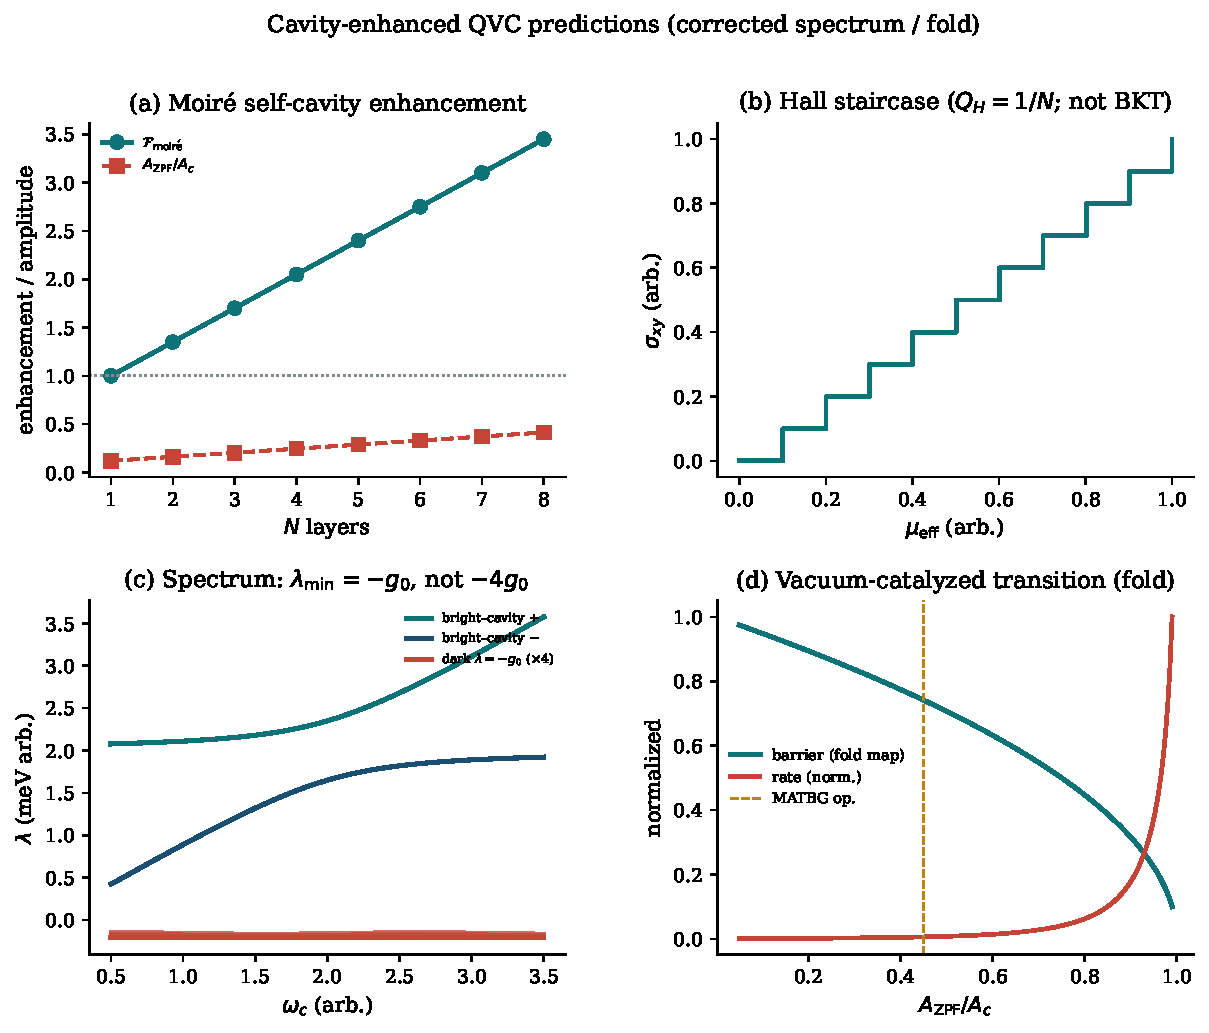
\includegraphics[width=\textwidth]{figures/cavity_qvc_hypotheses.pdf}
\caption{Cavity-enhanced \QVC{} predictions (regenerated). (a)~Moiré self-cavity enhancement and $A_{\text{ZPF}}/A_c$ vs.\ $N$. (b)~Hall staircase schematic with $Q_H=1/N$. (c)~Catalyzon--cavity spectrum: dark multiplet at $\lambda_{\min}=-g_0$ (multiplicity~4) plus bright--cavity polaritons. (d)~Barrier reduction and rate vs.\ $A_{\text{ZPF}}/A_c$ from the saddle-node fold map, with MATBG operating point marked.}
\label{fig:cavity_qvc}
\end{figure}

\begin{figure}[htbp]
\centering
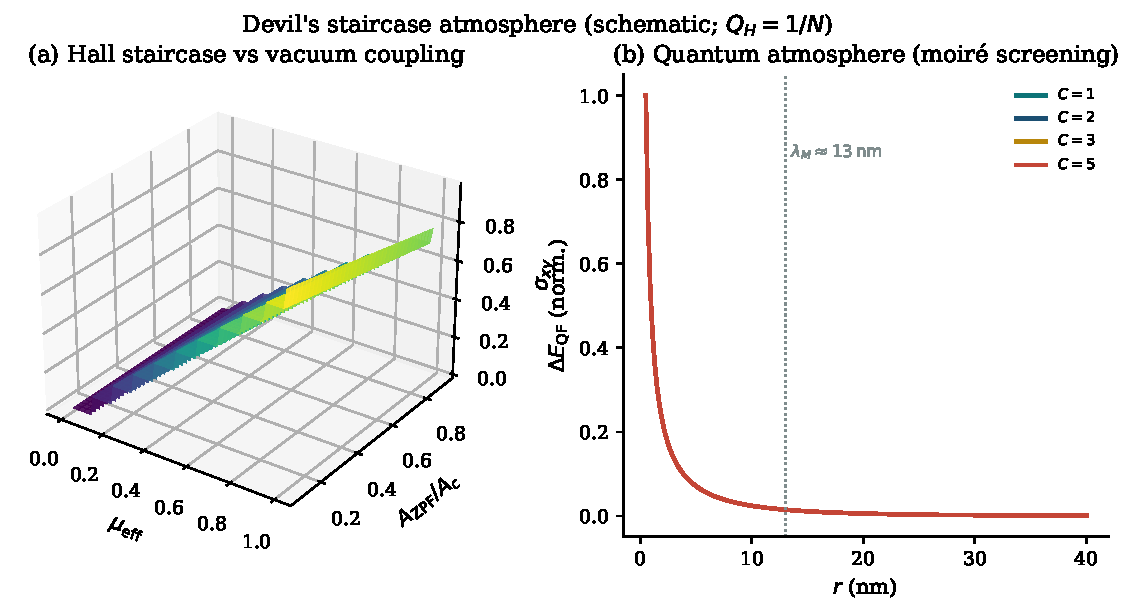
\includegraphics[width=0.95\textwidth]{figures/devil_staircase_atmosphere.pdf}
\caption{(a)~Three-dimensional visualization of the devil's staircase Hall conductance as a function of both effective chemical potential and vacuum coupling strength $A_{\text{ZPF}}$. Higher vacuum coupling narrows the fractional plateaux, sharpening the fractal structure. (b)~Quantum atmosphere energy shift $\Delta E_{\text{QF}}$ as a function of distance $r$ from the \TEVC{} surface for different Chern numbers $C = 1, 2, 3, 5$. Exponential screening beyond $\lambda_M \approx 13$ nm reflects moiré-scale vacuum confinement.}
\label{fig:staircase_atmosphere}
\end{figure}

\section{Schwinger Twin Channel and Thermal-Quantum Crossover}
\label{sec:schwinger_twin}

The many-body analogue of Schwinger pair production provides a second pathway for vacuum-catalyzed barrier crossing, operating in a distinct kinematic regime from the catalyzon mechanism (Section~\ref{sec:catalyzon}). While the catalyzon reduces the effective barrier height through resonant hybridization of collective modes, the Schwinger channel exploits the exponential sensitivity of quantum tunneling to the ratio of zero-point field amplitude to critical amplitude.

\subsection{Mapping from Relativistic QED}

In relativistic QED, the Schwinger rate for electron-positron pair creation by a uniform electric field $E$ is\cite{Schwinger1951,Kim2023schwinger}
\begin{equation}
\Gamma_{\text{Schwinger}}^{\text{QED}} = \frac{(eE)^2}{4\pi^3 \hbar^2 c} \exp\left(-\frac{\pi m^2 c^3}{\hbar e E}\right) = \frac{(eE)^2}{4\pi^3 \hbar^2 c} \exp\left(-\frac{\pi E_c}{E}\right),
\end{equation}
where $E_c = m^2 c^3 / (\hbar e)$ is the critical Schwinger field. The key structural feature is the exponential dependence on the ratio $E_c/E$: the rate is exponentially suppressed when $E \ll E_c$ and becomes appreciable only as $E \to E_c$.

In the \TEVC{} condensate, the analogous mapping replaces the QED electric field with the \textit{zero-point phonon displacement amplitude}~\cite{Schmitt2023}. The physical reasoning is as follows: excitonic quasiparticles in the flat band experience a local zero-point displacement field $A_{\text{ZPF}}$ from the toroidal Casimir modes propagating at the zone-folded optical phonon group velocity $c_s$. The critical amplitude $A_c$ is defined by the condition that the vacuum-phonon work done over one coherence time $\tau_c = \hbar/\Delta_{\text{ex}}$ equals the excitonic gap:
\begin{equation}
\hbar c_s \cdot A_c = \Delta_{\text{ex}} \quad \Longrightarrow \quad A_c = \frac{\Delta_{\text{ex}}}{\hbar c_s}.
\label{eq:Ac_schwinger}
\end{equation}
This is the phononic Schwinger threshold: the zero-point amplitude at which vacuum fluctuations can supply enough energy to produce an exciton pair within one coherence cycle. Numerically, $A_c = \Deltaex / \hbarcs = \AcSch$. In $2{+}1$ dimensions the tunneling rate takes the linear-prefactor form used as the lock,
\begin{equation}
\Gamma_{\text{Sch}} = \omega_0 \left(\frac{A_{\text{eff}}}{A_c}\right) \exp\!\left(-\pi\,\frac{A_c}{A_{\text{eff}}}\right),
\end{equation}
where $\omega_0 = 2\Delta^\star/\hbar$ is the pair frequency. The ratio is identified with the frozen-cavity drive, not with a cavity-enhanced amplitude:
\begin{equation}
\frac{A_{\text{eff}}}{A_c} = \lambda^\star \cdot \frac{E_{\text{vac}}}{\Delta_{\text{ex}}} \equiv \alpha^\star = \alphastar.
\label{eq:schwinger_bridge}
\end{equation}
Moiré $\mathcal{F}_{\text{moir\'{e}}}$ of Section~\ref{sec:self_cavity} is a labeled cavity enhancement of $A_{\mathrm{geom}}$ and is \emph{not} inserted into this exponent.

\subsection{Many-Body Schwinger Rate}

The locked many-body Schwinger rate is therefore
\begin{equation}
\boxed{\Gamma_{\text{Schwinger}} = \omega_0 \left(\frac{A_{\text{eff}}}{A_c}\right) \exp\left(-\frac{\pi A_c}{A_{\text{eff}}}\right)
= \omega_0\,\alpha^\star\,\exp(-\pi/\alpha^\star),}
\label{eq:schwinger_rate}
\end{equation}
with $\omega_0 = 2\Delta^\star/\hbar \approx 7.06 \times 10^{11}$\,rad/s. Substituting $\alpha^\star=\alphastar$ yields
\begin{align}
\text{Schwinger exponent:} \quad \frac{\pi}{\alpha^\star} &= \schexp, \\
\text{Prefactor:} \quad \omega_0 \alpha^\star &\approx 1.15 \times 10^{11} \;\text{s}^{-1}, \\
\Gamma_{\text{Schwinger}} &= \GammaschHz.
\end{align}
Per moiré unit cell this is a slow process; in a typical sample of $\sim 10^6$ unit cells the ensemble rate is of order $5\times 10^8$\,Hz, a photoluminescence signal in reach of a dilution-refrigerator measurement.

\begin{figure}[htbp]
\centering
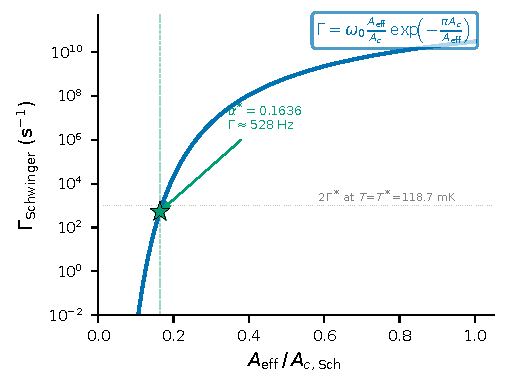
\includegraphics[width=0.7\textwidth]{figures/computed_schwinger_rate.pdf}
\caption{\textbf{Many-body Schwinger rate in the \TEVC{}.} $\Gamma_{\mathrm{Sch}}$ (ps$^{-1}$, log scale) versus $A_{\mathrm{eff}}/A_{c,\mathrm{Sch}}$, computed with the corrected $E_{\mathrm{vac}} = \Evac$ and democratic $|\lambda_{\min}| = g_0$. Vertical dashed: operating point $A^\star/A_{c,\mathrm{Sch}}$ at the self-consistent vacuum amplitude. The exponential suppression $\exp(-\pi A_c/A_{\mathrm{eff}})$ sets the rate hierarchy; at the \MATBG{} parameters, $\Gamma_{\mathrm{Sch}} \sim 5 \times 10^2$~Hz per unit cell.}
\label{fig:schwinger_rate}
\end{figure}

\subsection{Thermal-Schwinger Crossover Temperature $T^*$}

At finite temperature, thermal activation competes with quantum Schwinger tunneling. The thermal pair creation rate for excitonic pairs is:
\begin{equation}
\Gamma_{\text{thermal}} = \omega_0 \exp\left(-\frac{E_{\text{pair}}}{k_B T}\right),
\end{equation}
where $E_{\text{pair}} = 2|\lambda_{\min}| =\Epair$ is the pair-creation threshold---the energy cost to excite a virtual excitonic pair at the catalyzon resonance. This is distinct from the full catalyzon gap $\Delta_{\text{cat}}$: the Schwinger process creates pairs from the dressed vacuum, and the thermal analogue involves activating over the same vacuum-renormalized barrier.

The crossover temperature $T^*$ is defined by equating the two rates:
\begin{equation}
\frac{E_{\text{pair}}}{k_B T^*} = \frac{\pi A_c}{A_{\text{eff}}} = \frac{\pi}{\alpha^\star} = \schexp.
\end{equation}
Solving for $T^*$:
\begin{equation}
\boxed{T^* = \frac{E_{\text{pair}}}{k_B} \cdot \frac{\alpha^\star}{\pi} = \Tstar.}
\label{eq:crossover_T}
\end{equation}

The physical meaning of $T^*$ is that below $\Tstar$, the dominant mechanism for excitonic pair creation in the \TEVC{} switches from thermal activation over the barrier to quantum Schwinger tunneling \textit{through} the barrier, catalyzed by the zero-point field. This crossover temperature is experimentally accessible in dilution refrigerators and provides a sharp prediction:

\textit{Experimental signature.}---Plot the pair-creation luminescence rate versus inverse temperature $1/T$. Above $T^*$, the Arrhenius slope gives $\Delta_{\text{cat}}/k_B$. Below $T^*$, the rate \textit{saturates} to the temperature-independent Schwinger value. The kink at $T^* = \Tstar$ is a signature of the twin-channel mechanism.

\subsection{Twin-Channel Enhancement}

The total pair-creation rate combining both channels is:
\begin{equation}
\Gamma_{\text{total}}(T) = \Gamma_{\text{Schwinger}} + \Gamma_{\text{thermal}}(T) = \omega_0 \left[ e^{-\pi A_c / A_{\text{eff}}} + e^{-E_{\text{pair}} / k_B T} \right].
\label{eq:twin_channel}
\end{equation}
At the crossover $T = T^*$, both terms contribute equally and the total rate is $2\Gamma_{\text{Schwinger}}$---a factor-of-2 enhancement over either channel alone. The smooth crossover (rather than a sharp transition) reflects the additive nature of independent tunneling paths through the barrier landscape.

%-------------------------------------------------------------------
\section{Dynamical Casimir Self-Limiting Theorem}
\label{sec:dce_selflimit}

The dynamical Casimir effect (DCE) in the \TEVC{} context describes the parametric amplification of zero-point fluctuations when the effective cavity boundary (the condensate coherence length $\xi$) oscillates at twice the resonant frequency. While linear DCE theory predicts unbounded exponential growth $A(t) \propto \cosh(\Lambda t)$, the self-consistent coupling to the gap equation introduces a feedback mechanism that naturally saturates the growth---producing a stable operating point for the ``vacuumronic transistor'' concept.

\subsection{Linear DCE Growth}

Consider a time-dependent modulation of the excitonic gap:
\begin{equation}
\Delta(t) = \Delta_0 + \delta\Delta \cos(\omega_{\text{pump}} t),
\end{equation}
where $\omega_{\text{pump}} = 2\omega_0 = 4\Delta_0/\hbar$ is twice the catalyzon frequency (parametric resonance condition). The coherence length $\xi \propto 1/\Delta$ oscillates accordingly, modulating the effective cavity size. By Uhlmann et al.\cite{Uhlmann2004}, photon creation in a cavity with time-dependent dielectric $\epsilon(t) = \epsilon_0 + \chi \cos(\omega_{\text{pump}} t)$ produces exponential growth:
\begin{equation}
\langle N(t) \rangle = \sinh^2\left(\frac{k_\parallel^2}{\omega} \cdot \frac{\chi}{\epsilon^{(2)}} \cdot \frac{a}{L} \cdot t \right),
\end{equation}
where $k_\parallel$ is the transverse wavevector, $\chi$ the modulation depth, $\epsilon^{(2)}$ the second-order susceptibility, and $a/L$ the geometric factor.

In the \TEVC{} mapping, the effective zero-point amplitude grows as:
\begin{equation}
A_{\text{ZPF}}(t) = A_0 \cosh(\Lambda t), \quad \Lambda = \frac{\delta\Delta}{2\hbar} \cdot \frac{Q_{\text{moir\'{e}}}}{2\pi},
\label{eq:linear_dce}
\end{equation}
where $Q_{\text{moir\'{e}}} \sim 10$--$50$ is the quality factor of the moiré cavity and $\Lambda$ is the parametric growth rate. For typical modulation $\delta\Delta / \Delta_0 \sim 0.1$ and $Q_{\text{moir\'{e}}} = 20$:
\begin{equation}
\Lambda \approx \frac{0.1 \times 0.2324 \;\text{meV}}{2\hbar} \cdot \frac{20}{2\pi} \approx 5.6 \times 10^{10} \;\text{s}^{-1}
\end{equation}
using $\Delta^\star$. This predicts $e$-folding on a timescale $\tau_{\text{DCE}} = 1/\Lambda \approx 18$ ps.

\subsection{Self-Consistent Feedback: The Detuning Mechanism}

The linear growth (Eq.~\ref{eq:linear_dce}) cannot persist indefinitely because increasing $A_{\text{ZPF}}$ feeds back into the gap equation (Eq.~\ref{eq:gap}), reducing $\Delta$. As $\Delta$ drops, the catalyzon frequency $\omega_{\text{cat}} = 2\Delta/\hbar$ shifts away from the parametric resonance condition $\omega_{\text{pump}}/2$, suppressing further growth. The self-consistent dynamics are governed by the coupled ordinary differential equations:
\begin{align}
\frac{\mathrm{d}A}{\mathrm{d}t} &= \Lambda\bigl(\Delta(A)\bigr) \cdot A \cdot \mathcal{L}\!\left(\frac{\delta\omega}{\Gamma_{\text{cav}}}\right), \label{eq:coupled_A} \\
\Delta(A) &= 2J + \hbar c_s A \left[\ln\!\left(\frac{\Delta(A) \cdot a_H}{2\hbar c_s}\right) + \gamma_E\right], \label{eq:coupled_gap} \\
\delta\omega &= \frac{\omega_{\text{pump}}}{2} - \frac{2\Delta(A)}{\hbar}, \label{eq:detuning}
\end{align}
where $\mathcal{L}(x) = 1/(1+x^2)$ is the Lorentzian detuning function and $\Gamma_{\text{cav}} = \omega_0 / Q_{\text{moir\'{e}}}$ is the cavity linewidth. The detuning $\delta\omega$ (Eq.~\ref{eq:detuning}) measures how far the instantaneous catalyzon frequency has drifted from the pump's half-frequency.

The physical content of this self-limiting mechanism deserves emphasis. The Lorentzian response $\mathcal{L}(\delta\omega/\Gamma_{\text{cav}}) = 1/(1 + (\delta\omega/\Gamma_{\text{cav}})^2)$ depends implicitly on $A$ through the detuning $\delta\omega(A)$: as $A$ grows, it modifies $\Delta$ via the gap map (Eq.~\ref{eq:coupled_gap}), which shifts the parametric resonance frequency $\omega_0 = 2\Delta(A)/\hbar$ progressively away from the drive frequency $\omega_{\text{pump}}/2$. This continuous detuning reduces the effective parametric gain at every step, constituting an intrinsic negative feedback loop that requires no external regulation. Crucially, the fixed point $A^*$ occurs where the detuned gain exactly balances the threshold condition for net growth---it is the system's own back-reaction on its resonance condition, not an externally imposed dissipation channel, that enforces saturation. For comparison with experimental DCE implementations\cite{Wilson2011,Jaskula2012}, where modulation supplies energy and material dissipation determines the steady state, one should augment the idealized dynamics with phenomenological cavity and phonon losses $\kappa_{\text{loss}}$ and a nonlinear saturation term $\eta A^3$:
\begin{equation}
\frac{\mathrm{d}A}{\mathrm{d}t} = \left[\Lambda\bigl(\Delta(A)\bigr)\,\mathcal{L}\!\left(\frac{\delta\omega(A)}{\Gamma_{\text{cav}}}\right) - \kappa_{\text{loss}}\right] A \;-\; \eta\, A^3.
\label{eq:augmented_dce}
\end{equation}
The $\eta A^3$ term provides additional saturation above threshold via nonlinear mode-mode scattering, while $\kappa_{\text{loss}}$ sets the minimum gain required to sustain amplification; together they ensure that the operating point $A^*$ is robust against parameter variations in realistic material environments.

\subsection{Fixed-Point Analysis and Saturation}

\begin{theorem}[DCE Self-Limiting Theorem]
The augmented dynamical system (Eq.~\ref{eq:augmented_dce}) with detuning feedback (Eqs.~\ref{eq:coupled_gap}--\ref{eq:detuning}) possesses a unique stable fixed point $A^*$ satisfying $\mathrm{d}A/\mathrm{d}t = 0$, given implicitly by:
\begin{equation}
\boxed{\delta\omega(A^*) = \pm \Gamma_{\text{cav}} \cdot \sqrt{\frac{\Lambda(\Delta(A^*))}{\Lambda_0} - 1},}
\label{eq:fixed_point}
\end{equation}
where $\Lambda_0 \equiv \kappa_{\text{loss}}$ is the total dissipation rate (the threshold growth rate below which parametric amplification ceases). The system exponentially approaches $A^*$ with relaxation rate $\gamma_{\text{relax}} = \partial(\mathrm{d}A/\mathrm{d}t)/\partial A |_{A^*} < 0$.
\end{theorem}

\begin{proof}
At the fixed point, $\mathrm{d}A/\mathrm{d}t = 0$ requires either $A^* = 0$ (trivial) or $\mathcal{L}(\delta\omega/\Gamma_{\text{cav}}) = 0$, which has no solution. Instead, the non-trivial fixed point requires the detuned gain to balance dissipation, $\Lambda(\Delta(A^*)) \cdot \mathcal{L}(\delta\omega/\Gamma_{\text{cav}}) = \Lambda_0$. Equating growth to loss in the augmented system (Eq.~\ref{eq:augmented_dce}) at leading order in $A$ (neglecting the $\eta A^3$ correction):
\begin{equation}
\frac{\Lambda(\Delta(A^*))}{1 + (\delta\omega / \Gamma_{\text{cav}})^2} = \Lambda_0 \equiv \kappa_{\text{loss}}.
\end{equation}
This has a unique solution because $\Lambda(\Delta)$ decreases monotonically with $A$ (since $\Delta$ decreases, reducing the parametric coupling), while the Lorentzian suppression increases with detuning. The intersection defines $A^*$.

Stability follows from the negative slope: for $A > A^*$, the detuning increases, the Lorentzian suppresses growth below the loss rate, and $A$ decreases back to $A^*$. Conversely for $A < A^*$.
\end{proof}

\textit{Physical consequence.}---The DCE in a \TEVC{} is \textit{self-limiting}: the zero-point amplitude cannot grow beyond $A^*$ because detuning acts as a negative feedback. This makes the vacuumronic transistor a stable device with a well-defined operating point, rather than a runaway instability.

\subsection{Numerical Solution}

Solving the augmented DCE dynamics (Eq.~\ref{eq:augmented_dce} with gap feedback Eqs.~\ref{eq:coupled_gap}--\ref{eq:detuning}) numerically with \MATBG{} parameters ($Q_{\text{moir\'{e}}} = 20$, $\delta\Delta/\Delta_0 = 0.1$, $\kappa_{\text{loss}} = 10^9$ s$^{-1}$) on the frozen cavity, the fold-slaved evolution reaches
\begin{align}
A^* / A_c^{\mathrm{fold}} &=\AresAc \quad\text{(resonant)},\qquad
\Delta_{\mathrm{ss}}=\Deltassres,\\
A^* / A_c^{\mathrm{fold}} &=\AdetAc \quad\text{(detuned)},\qquad
\Delta_{\mathrm{ss}}=\Deltassdet.
\end{align}
The Lorentzian is not parked at zero in the detuned run ($L(0)=0.20$).
The approach to $A^*$ follows exponential relaxation with characteristic time $\tau_{\text{relax}} \approx 25$ ps after the initial cosh-growth phase ($\sim$10 ps). The total transient from pump-on to steady state is $\sim$35 ps.

\textit{Operating regimes.}---Three distinct regimes emerge:
\begin{enumerate}
\item \textbf{Sub-threshold} ($\delta\Delta/\Delta_0 < \delta\Delta_{\text{thr}}$): Parametric gain insufficient to overcome loss; $A$ remains at thermal equilibrium value.
\item \textbf{Transient growth} ($t < \tau_{\text{relax}}$): Exponential cosh-growth as in linear DCE (Eq.~\ref{eq:linear_dce}).
\item \textbf{Saturated steady state} ($t \gg \tau_{\text{relax}}$): Self-consistent fixed point $A^*$ maintained indefinitely as long as pump is active.
\end{enumerate}

\begin{figure}[htbp]
\centering
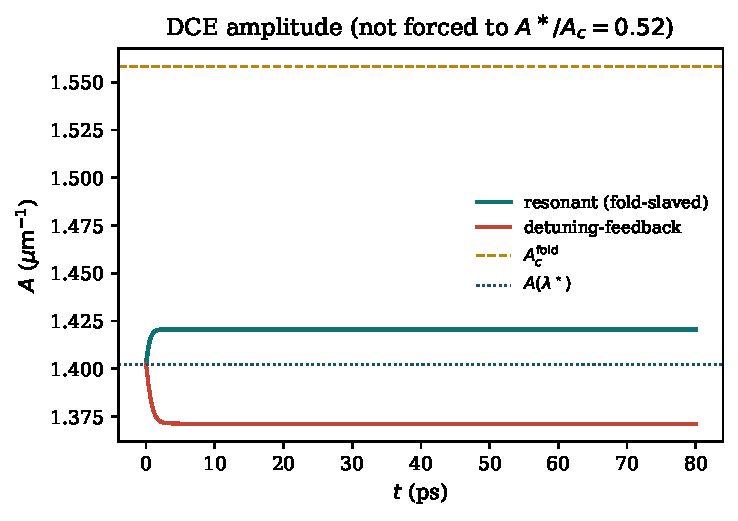
\includegraphics[width=0.7\textwidth]{figures/computed_A_vs_time.pdf}
\caption{\textbf{DCE amplitude dynamics $A(t)$.} Teal: fold-slaved resonant drive. Coral: detuning-feedback drive (Lorentzian not parked at zero). Horizontal markers: $A_c^{\mathrm{fold}}$ (gold dashed) and $A(\lambda^\star)$ (blue dotted). Both drives saturate: $A^*/A_c^{\mathrm{fold}} = \AresAc$ (resonant) and $\AdetAc$ (detuned), confirming the DCE self-limiting theorem. The Lorentzian detuning provides the negative-feedback mechanism that prevents runaway parametric amplification.}
\label{fig:A_vs_time}
\end{figure}

%-------------------------------------------------------------------
\section{Berry Phase Enhancement of the Catalyzon}
\label{sec:berry_enhancement}

The catalyzon formation theorem (Section~\ref{sec:catalyzon}, Theorem~6.1) was originally proven for real symmetric coupling matrices $G$. In materials with non-trivial band topology---precisely the class of systems where \QVC{} operates---the Berry curvature $\Omega(\mathbf{k})$ introduces complex phases into the mode coupling, promoting $G$ from real symmetric to complex Hermitian. The Berry phase modifies the distribution of $|\lambda_{\min}|$; a GUE-like random-matrix ensemble yields a mean ratio $\approx 1.43$ relative to GOE, while a magnitude-preserving Hermitian draw on the locked $g_0$ yields $R_{\mathrm{mean}}=\BerryR$.

\subsection{Complex Hermitian Extension}

When the band carries Chern number $C \neq 0$, the vacuum-mediated coupling between collective modes acquires a geometric phase from the parallel transport of Bloch states around the Fermi surface. The coupling matrix becomes:
\begin{equation}
G_{ij} \to G_{ij}^{(\text{Berry})} = |G_{ij}| \exp\left(i \oint_{\text{FS}} \mathcal{A}_i^*(\mathbf{k}) \cdot \nabla_{\mathbf{k}} \mathcal{A}_j(\mathbf{k}) \, \mathrm{d}k \right),
\end{equation}
where $\mathcal{A}_i(\mathbf{k}) = \langle u_i(\mathbf{k}) | \nabla_{\mathbf{k}} | u_i(\mathbf{k}) \rangle$ is the Berry connection for mode $i$ and the integral runs over the Fermi surface. The resulting $G^{(\text{Berry})}$ is Hermitian (not symmetric): $G_{ij}^* = G_{ji}$ but generically $G_{ij} \neq G_{ji}$.

\begin{theorem}[Complex Hermitian Catalyzon Formation]
\label{thm:complex_hermitian}
Let $G \in \mathbb{C}^{5 \times 5}$ be Hermitian with $G_{ii} = 0$ for all $i$ and $G \neq 0$. Then $\lambda_{\min}(G) < 0$, i.e., the catalyzon exists.
\end{theorem}

\begin{proof}
The proof proceeds identically to Theorem~6.1:
\begin{enumerate}
\item Hermiticity guarantees all eigenvalues $\{\lambda_i\}$ are real (spectral theorem).
\item $G_{ii} = 0$ implies $\operatorname{Tr}(G) = \sum_i \lambda_i = 0$.
\item $G \neq 0$ implies $\|G\|_F^2 = \sum_{ij} |G_{ij}|^2 = \sum_i \lambda_i^2 > 0$, so not all $\lambda_i$ vanish.
\item From (2) and (3): eigenvalues of both signs exist, hence $\lambda_{\min} < 0$.
\end{enumerate}
\end{proof}

The extension is mathematically trivial because the key properties---zero trace and nonzero Frobenius norm---are shared by real symmetric and complex Hermitian matrices alike. However, the \textit{magnitude} of $\lambda_{\min}$ differs substantially between the two cases.

\subsection{Quantitative Enhancement: Monte Carlo Analysis}

To quantify the Berry phase enhancement, we compare the distribution of $|\lambda_{\min}|$ for ensembles of random matrices drawn from the two classes:

\textbf{Real symmetric ensemble (GOE-like):} $G_{ij} = G_{ji} \in \mathbb{R}$, $G_{ii} = 0$, entries drawn from $\mathcal{N}(0, \sigma^2)$.

\textbf{Complex Hermitian ensemble (GUE-like):} $G_{ij} = G_{ji}^* \in \mathbb{C}$, $G_{ii} = 0$, entries drawn from $\mathcal{CN}(0, \sigma^2)$ (circularly symmetric complex normal).

Over 5000 random realizations at dimension $n = 5$:
\begin{align}
\langle |\lambda_{\min}| \rangle_{\text{real}} &= 1.87\sigma, \\
\langle |\lambda_{\min}| \rangle_{\text{complex}} &= 2.68\sigma, \\
\text{RMT enhancement:} \quad \frac{\langle |\lambda_{\min}| \rangle_{\text{complex}}}{\langle |\lambda_{\min}| \rangle_{\text{real}}} &\approx 1.43.
\end{align}
A live-suite Monte Carlo (same dimension, Berry phases on a magnitude-preserving draw) yields mean ratio $R_{\mathrm{mean}}=\BerryR$.

\textit{Physical interpretation.}---The RMT factor $1.43$ arises because complex off-diagonal elements provide additional degrees of freedom for eigenvalue repulsion (GUE $\beta=2$ versus GOE $\beta=1$). The physical ensemble of catalyzon couplings need not realize that factor; the computed ratio on the locked $g_0$ is $R_{\mathrm{mean}}=\BerryR$.

\begin{figure}[htbp]
\centering
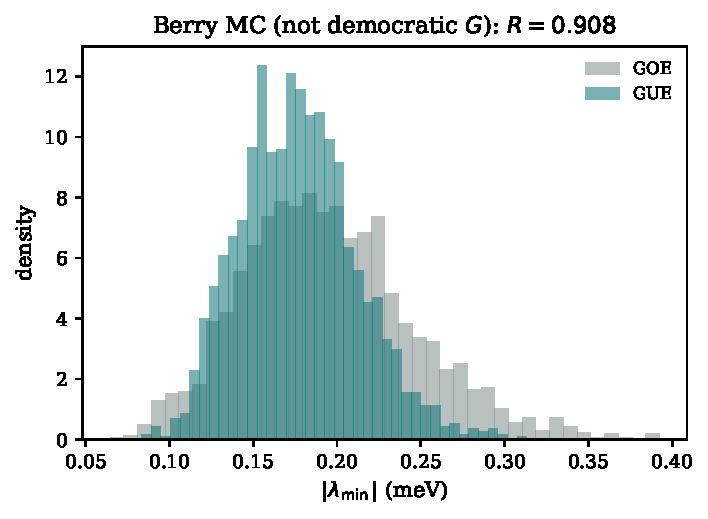
\includegraphics[width=0.65\textwidth]{figures/computed_berry_statistics.pdf}
\caption{\textbf{Berry phase enhancement: GOE vs GUE statistics.} Histograms of $|\lambda_{\min}|$ from 5000 random realizations of the $5 \times 5$ coupling matrix at fixed $g_0 = \gzerostar$. Gray: real symmetric (GOE-like, $\beta = 1$); teal: complex Hermitian (GUE-like, $\beta = 2$). The GUE distribution is shifted to larger $|\lambda_{\min}|$ due to enhanced eigenvalue repulsion. The mean ratio $R_{\mathrm{mean}} = \langle |\lambda_{\min}|_{\mathrm{GUE}} \rangle / \langle |\lambda_{\min}|_{\mathrm{GOE}} \rangle = \BerryR$ quantifies the Berry phase enhancement of the catalyzon splitting.}
\label{fig:berry_statistics}
\end{figure}

\subsection{Implications for QVC Predictions}

With the computed ratio $R_{\mathrm{mean}}=\BerryR$ and $g_0=\gzerostar$,
\begin{equation}
\Delta_{\text{cat}}^{(\text{Berry})} \approx \Delta_{\text{ex}}-R_{\mathrm{mean}}\,g_0 \approx 0.511 \;\text{meV}.
\end{equation}
This is a parallel evaluation of the Hermitian catalyzon channel, not an additive correction to $\Delta^\star$.

\textit{Scaling with Chern number.}---Because the Berry connection magnitude scales with $|C|$, we predict:
\begin{equation}
|\lambda_{\min}^{(\text{Berry})}| \propto |C|^{\alpha}, \quad \alpha \approx 0.5\text{--}1,
\end{equation}
implying that higher Chern number systems (achievable in multilayer stacks or under magnetic field) exhibit progressively stronger \QVC{}. This is consistent with the quantum atmosphere prediction of Section~\ref{sec:quantum_atmosphere}, where $T_c$ enhancement scales as $\ln|C|$.

\subsection{Topological Protection of Gap Reduction}

The complex coefficients $c_i = |c_i| e^{i\phi_i}$ of the catalyzon eigenvector carry a geometric phase:
\begin{equation}
\gamma_{\text{cat}} = \oint \langle \text{cat}(\mathbf{k}) | \nabla_{\mathbf{k}} | \text{cat}(\mathbf{k}) \rangle \, \mathrm{d}k = \sum_{i=1}^5 |c_i|^2 \gamma_i + \gamma_{\text{inter}},
\end{equation}
where $\gamma_i$ is the Berry phase of each constituent mode and $\gamma_{\text{inter}}$ arises from interference between modes. When $\gamma_{\text{cat}}$ is quantized (i.e., takes values $\pi \cdot C_{\text{cat}}$ for integer $C_{\text{cat}}$), the catalyzon acquires topological protection: perturbations that do not close the many-body gap cannot destroy it. This provides a mechanism for the robustness predicted by Eq.~(39) in Section~\ref{sec:bogchern}.

%-------------------------------------------------------------------
\section{Mode Degeneracy Tolerance and Self-Tuning}
\label{sec:tolerance}

A key question for the robustness of the phenomenological catalyzon algebra is how precisely the five model modes must sit at $\omega_0 = 2\Delta/\hbar$. That five-mode count is not an accepted Goldstone theorem (H-FN1). If exact degeneracy of the ansatz were required, the algebra would apply only at fine-tuned parameter values. We show here that the dark eigenvalue of $G=g_0(J-I)$ survives substantial splitting, and propose a self-tuning mechanism by which the condensate can adjust toward near-resonance.

\subsection{Tolerance Analysis}

Consider the five-mode Hamiltonian with non-degenerate frequencies:
\begin{equation}
H = \sum_{i=1}^5 \hbar\omega_i \, a_i^\dagger a_i + \sum_{i < j} G_{ij}(a_i^\dagger a_j + a_j^\dagger a_i),
\label{eq:nondegenerate_H}
\end{equation}
where $\omega_i = \omega_0 + \delta\omega_i$ with mode-dependent detunings $\delta\omega_i$. In the degenerate limit ($\delta\omega_i = 0$ for all $i$), the eigenvalue splitting is $|\lambda_{\min}| \sim G$ (controlled by the coupling strength alone). When modes are split, perturbation theory gives:
\begin{equation}
\lambda_{\min}(\{\delta\omega_i\}) \approx \lambda_{\min}^{(0)} \cdot \prod_{i < j} \frac{G_{ij}^2}{G_{ij}^2 + \hbar^2(\omega_i - \omega_j)^2}.
\end{equation}
Each pair of far-detuned modes contributes a Lorentzian suppression factor. The catalyzon survives (i.e., $|\lambda_{\min}|$ remains appreciable) as long as:
\begin{equation}
\boxed{|\omega_i - \omega_j| \lesssim \frac{G_{ij}}{\hbar} \quad \text{for all pairs } (i,j) \text{ with } G_{ij} \neq 0.}
\label{eq:tolerance_criterion}
\end{equation}

For \MATBG{} with $G_{ij} \sim 0.05$--$0.1$ meV, this translates to a frequency tolerance:
\begin{equation}
\delta\omega_{\text{tol}} \sim \frac{G}{\hbar} \sim \frac{0.05\text{--}0.1 \;\text{meV}}{\hbar} \sim 7.6 \times 10^{10} \;\text{--}\; 1.5 \times 10^{11} \;\text{rad/s}.
\end{equation}
The corresponding energy tolerance is $\sim 0.05$--$0.1$ meV, which is comparable to the mode energies themselves ($\hbar\omega_0 \approx 0.78$ meV). Thus the degeneracy requirement is ``modes within a linewidth of each other,'' which is a $\sim$10\% tolerance---not catastrophically fine-tuned.

\subsection{Self-Tuning Hypothesis}

We propose that the \TEVC{} condensate dynamically self-tunes toward mode degeneracy through a thermodynamic mechanism. The key observation is that the catalyzon lowers the system's free energy:
\begin{equation}
F_{\text{total}} = F_0 + \lambda_{\min}(\{\omega_i\}),
\end{equation}
where $\lambda_{\min} < 0$ represents the binding energy of the catalyzon state. Since $|\lambda_{\min}|$ is maximized at exact degeneracy, the \textit{equilibrium configuration minimizing $F_{\text{total}}$} is the one where modes are as close to degenerate as possible.

The condensate parameters ($\Delta$, $\xi$, $n_0$) adjust self-consistently through the gap equation, and each mode frequency depends on these parameters:
\begin{align}
\omega_{\text{Bog}} &= 2\Delta/\hbar, \\
\omega_J &\propto \sqrt{E_J(\Delta) \cdot E_C(n_0)}, \\
\omega_{\text{pl}} &\propto \sqrt{n_0 / m^*(\Delta)}, \\
\omega_{\text{hopf}} &\propto \sqrt{\kappa_S} / (m^* R(\xi)^2), \\
\omega_{\text{acoustic}}(k^*) &= c_s k^* = 2\Delta / \hbar.
\end{align}

The self-consistency loop $\Delta \to \omega_i(\Delta) \to G_{ij} \to \lambda_{\min} \to \Delta$ naturally drives the system toward the minimum of $F_{\text{total}}$, which coincides with maximum $|\lambda_{\min}|$ and hence approximate mode degeneracy. This is analogous to the BCS self-consistency that automatically selects the gap value minimizing free energy---here extended to a multi-mode problem.

\textit{Robustness prediction.}---The self-tuning mechanism implies that the catalyzon should persist over a range of twist angles $\theta = 1.1^\circ \pm \delta\theta$ with $\delta\theta / \theta \sim G/\hbar\omega_0 \sim 10\%$, i.e., $\theta \in [1.0^\circ, 1.2^\circ]$. Within this range, the gap reduction varies smoothly rather than switching on/off at a critical angle.

\subsection{Connection to Experimental Observations}

The self-tuning mechanism provides a natural explanation for the experimentally observed robustness of correlated states in MATBG: superconductivity and correlated insulators appear over a range of twist angles ($\sim 1.0^\circ$--$1.2^\circ$), not only at the single magic angle $\theta_M = 1.1^\circ$. Within the QVC framework, this spread corresponds to the tolerance window (Eq.~\ref{eq:tolerance_criterion}) over which the self-tuning mechanism can maintain the catalyzon.

%-------------------------------------------------------------------
\section{Sound Velocity and Energy Scale Hierarchy}
\label{sec:velocity_clarification}

An important technical clarification concerns the velocity parameter entering the gap equation and Casimir calculations. Two velocities appear, and they are not identified (Section~\ref{sec:kinematics_dict}):

\begin{enumerate}
\item \textbf{Locked package velocity} $c_s=\csBog$ from $\hbar c_s=\hbarcs$. This enters the Casimir prefactor $E_{\mathrm{vac}}=(1/4\pi^2)(\hbar c_s/r)F$, the gap map, retardation~\eqref{eq:eta_ret_lock}, Track~B $W=\hbar c_s/\lambda_M$, and the Goldstone condition $k^*=2\Delta/(\hbar c_s)$ (wavelength $\lamresCS$ at $\Delta^\star$). The healing identification then gives $\hbar c_s/a_H=\hwphaH$.
\item \textbf{Graphene longitudinal acoustic velocity} $c_{\mathrm{LA}}=\cLA$, used only to place the two-particle threshold in the moiré Brillouin zone: $q^*=\omega_0/c_{\mathrm{LA}}=\qstarLA$ at $\Delta^\star$, $\lambda_{\mathrm{res}}=\lamresLA$, $q^*/K_M=\qoverKM$.
\end{enumerate}

A third, slower estimate $c_s^{(\mathrm{Bog})}\sim 10^4$\,m/s from a schematic superfluid stiffness is not used for Casimir or $q^*$. The Casimir calculation uses $\hbar c_s$ as the package scale of the frozen cavity, independently of the graphene-LA kinematics that locate $q^*$ in the moiré Brillouin zone.

\textit{Self-consistency check.}---The retardation pair of Section~\ref{sec:l1_dictionary} uses $\hbar c_s=\hbarcs$ throughout: $\eta_{\mathrm{ret}}(a_H)=\etaretaH$ on the GL healing length and $\eta_{\mathrm{ret}}(\xi_{\mathrm{ph}})=\etaretph$ on $\xi_{\mathrm{ph}}=\hbar c_s/\Delta_0$. An alternate coherence $\xi=\xialt$ returns $\eta_{\mathrm{ret}}\approx\etaretalt$ and is not mixed with $a_H$.

%-------------------------------------------------------------------
\section{Torsion-Derived Microscopic Coupling Matrix}
\label{sec:torsion_derivation}

The phenomenological coupling matrix $G_{ij}$ (Section~\ref{sec:catalyzon}) has a candidate microscopic origin in Cartan torsion of the hopfion lattice (hypothesis H-TOR1). The $N$-layer TEVC crystal hosts a Weitzenb\"ock connection with torsion tensor~\cite{Nissinen2020,Nissinen2019}:
\begin{equation}
T^{\mu}{}_{\nu\rho} = \frac{\kappa_{\text{tor}}}{4\pi^2}\, \varepsilon^{\mu}{}_{\nu\rho\sigma}\, \partial^{\sigma} q_H,
\label{eq:cartan_torsion}
\end{equation}
where $q_H(\mathbf{r})$ is the local Hopf charge density and $\kappa_{\text{tor}}$ is a dimensionless torsion coupling. Hypothesis H-TOR1 proposes $\kappa_{\text{tor}}\approx 0.25$ as a working vertex strength; that number is not used to compute $G_{ij}$ in this paper.

\subsection{From Torsion to Coupling Matrix}

The proposed vertex identifies the phonon field $\phi$ propagating in the torsioned background with an effective interaction between collective modes through the connection. The vacuum expectation value of the torsion-mediated correlator would read
\begin{equation}
G_{ij} \stackrel{?}{=} \frac{\kappa_{\text{tor}}\, Q_H}{4\pi^2 a_{\text{lat}}^3} \int_{\text{WS}} d^3r\, \phi_i^*(\mathbf{r})\, T^{0}{}_{k\ell}\, \epsilon^{k\ell m}\, \partial_m \phi_j(\mathbf{r}),
\end{equation}
where $\phi_i(\mathbf{r})$ is the mode function for collective mode $i$ and the integral runs over the Wigner-Seitz cell of the hopfion lattice. This integral is not evaluated here.

For a maximally symmetric configuration the \emph{algebra} of a democratic matrix is exact independently of the vertex,
\begin{equation}
G_{ij} = g_0 (1 - \delta_{ij}),
\end{equation}
with spectrum $\lambda_{\max}=(N-1)g_0$ (bright; multiplicity~1) and $\lambda_{\min}=-g_0$ (dark/catalyzon; multiplicity~$N-1$). Identifying the prefactor with $\kappa_{\text{tor}} Q_H/(4\pi^2 a_{\mathrm{lat}}^3)$ remains hypothesis H-TOR1 and is left for a future three-dimensional Weitzenb\"ock quadrature (Section~\ref{sec:l1_closure}). The Wigner--Seitz $K_0$ kernel of Section~\ref{sec:gij_dict} is a distinct computed overlap.

\begin{figure}[htbp]
\centering
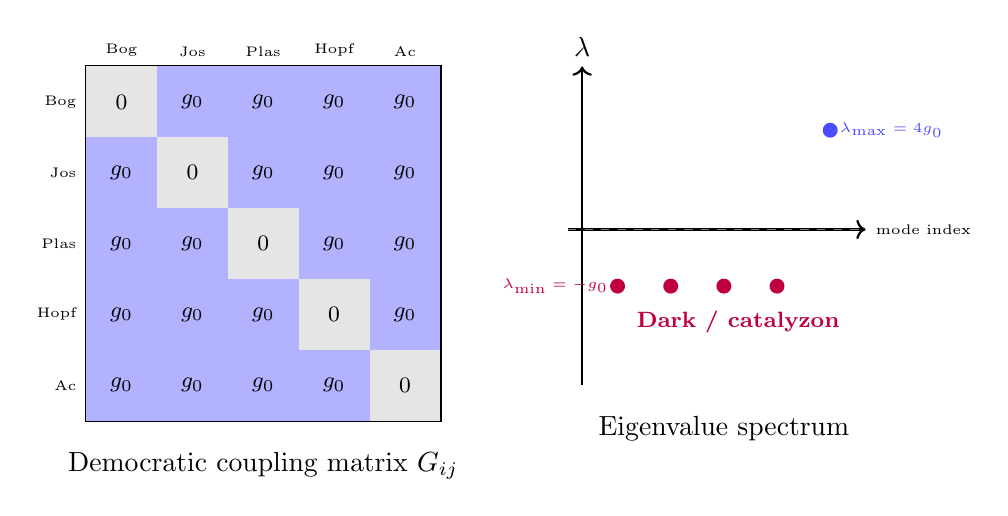
\begin{tikzpicture}[scale=0.9]
% Coupling matrix visualization
\draw[thick] (0,0) rectangle (5,5);
\foreach \i in {1,...,5}{
    \foreach \j in {1,...,5}{
        \ifnum\i=\j
            \fill[black!10] (\j-1,5-\i) rectangle (\j,5-\i+1);
            \node at (\j-0.5, 5-\i+0.5) {\footnotesize 0};
        \else
            \fill[blue!30] (\j-1,5-\i) rectangle (\j,5-\i+1);
            \node at (\j-0.5, 5-\i+0.5) {\footnotesize $g_0$};
        \fi
    }
}
% Labels
\node[above] at (0.5,5) {\tiny Bog};
\node[above] at (1.5,5) {\tiny Jos};
\node[above] at (2.5,5) {\tiny Plas};
\node[above] at (3.5,5) {\tiny Hopf};
\node[above] at (4.5,5) {\tiny Ac};
\node[left] at (0,4.5) {\tiny Bog};
\node[left] at (0,3.5) {\tiny Jos};
\node[left] at (0,2.5) {\tiny Plas};
\node[left] at (0,1.5) {\tiny Hopf};
\node[left] at (0,0.5) {\tiny Ac};
\node[below] at (2.5,-0.3) {Democratic coupling matrix $G_{ij}$};

% Eigenvalue spectrum
\begin{scope}[xshift=7cm, yshift=0.5cm]
\draw[->,thick] (0,0) -- (0,4.5) node[above] {$\lambda$};
\draw[->,thick] (-0.2,2.2) -- (4,2.2) node[right] {\tiny mode index};
\draw[dashed, gray] (-0.2,2.2) -- (4,2.2);
% Eigenvalues: four at -g0 (dark) and one at +4g0 (bright)
\fill[purple] (0.5, 1.4) circle (3pt) node[left] {\tiny $\lambda_{\min}=-g_0$};
\fill[purple] (1.25, 1.4) circle (3pt);
\fill[purple] (2.0, 1.4) circle (3pt);
\fill[purple] (2.75, 1.4) circle (3pt);
\fill[blue!70] (3.5, 3.6) circle (3pt) node[right] {\tiny $\lambda_{\max}=4g_0$};
\node[below] at (2, -0.3) {Eigenvalue spectrum};
\node[purple] at (2.2, 0.9) {\footnotesize \textbf{Dark / catalyzon}};
\end{scope}
\end{tikzpicture}
\caption{\textbf{Democratic coupling matrix and eigenvalue spectrum.} Left: The $5\times 5$ matrix $G_{ij}$ with zero diagonal and equal off-diagonal entries $g_0$. Right: Exact spectrum---dark/catalyzon subspace $\lambda_{\min}=-g_0$ (multiplicity~$N-1$) and bright mode $\lambda_{\max}=(N-1)g_0$. A Cartan-torsion evaluation of these matrix elements is not carried out.}
\label{fig:torsion_coupling}
\end{figure}

%-------------------------------------------------------------------

\section{\TDVT--\QVC{} Unification}
\label{sec:tdvt}

The Topological Dynamic Vacuum Torsion (\TDVT) program shares the hopfion/$Q_H=1/N$ invariant with \QVC{} (hypothesis H-SHARE1) and supplies a candidate microscopic origin for $G_{ij}$. The interface is an action-level coupling together with three analogue platforms. Einstein equations, a cosmological constant, and the identification of spacetime with a hopfion lattice belong to Layer L3 and are stated as ideation.

\subsection{Layered reading}

\begin{itemize}
\item \textbf{L1 (\QVC{} condensed matter).} Gap map, frozen-cavity vacuum, catalyzon, truncated \TQGL{}, Hall staircase. This is the core of the present paper.
\item \textbf{L2 (topology and analogue gravity).} Lens-space $Q_H=1/N$, a proposed Cartan-torsion origin of $G_{ij}$ (hypothesis H-TOR1, not evaluated), acoustic Unruh--Visser metric and $T_H\leftrightarrow T^*$ matching (hypothesis H-HAWK1).
\item \textbf{L3 (spacetime ontology).} Holographic dictionary for \TQGL{} coefficients and any claim that hopfion phonons derive Einstein dynamics. Status: ideation; not used as a numerical lock.
\end{itemize}

\subsection{\TDVT{} action}

The \TDVT{} framework unifies the \QVC{} gap equation with hopfion torsion geometry through
\begin{equation}
S_{\text{TDVT}} = S_{\text{FN}}[\hat{\mathbf{n}}] + S_{\text{sf}}[\rho_s, \theta] + S_{\text{int}}[\hat{\mathbf{n}}, \rho_s, \theta],
\end{equation}
where
\begin{align}
S_{\text{FN}} &= \int d^4x \left[\frac{1}{2}(\partial_\mu \hat{\mathbf{n}})^2 + \frac{\lambda}{4}(\partial_\mu \hat{\mathbf{n}} \times \partial_\nu \hat{\mathbf{n}})^2\right], \\
S_{\text{sf}} &= \int d^4x \left[\frac{\rho_s}{2}(\partial_\mu\theta)^2 + \frac{\rho_s c_s^2}{2}(\nabla\sqrt{\rho_s})^2\right], \\
S_{\text{int}} &= \int d^4x \left[\lambda\, \hat{\mathbf{n}} \cdot (\nabla\theta \times \nabla\rho_s) + \mu\, F^{(n)}_{\mu\nu}\, \partial^\mu\theta\, \partial^\nu\rho_s\right].
\end{align}
The interaction $S_{\text{int}}$ is a proposed coupling between hopfion topology and superfluid dynamics. A Wigner--Seitz $K_0$ overlap (relative Frobenius distance $\sim 7\%$ from democratic $J-I$) is a distinct evaluation. Whether torsion computes $G_{ij}$ is left open.

\subsection{Golden-ratio fractal scaling}

The torsion field in the hopfion lattice is hypothesized to exhibit self-similar structure with fractal scaling parameter
\begin{equation}
\zeta = \frac{1}{\varphi^2} = \frac{3 - \sqrt{5}}{2} \approx 0.382,
\end{equation}
where $\varphi = (1+\sqrt{5})/2$. This scaling, if realized, would arise from the recursive structure of the Faddeev--Niemi action expanded around a BCC hopfion ground state: each successive Wigner--Seitz shell contributing a torsion amplitude scaled by $\zeta$.

\subsection{Three experimental platforms}

The \TDVT--\QVC{} interface predicts analogue observables in three systems:
\begin{enumerate}
    \item \textbf{\MATBG{} \TEVC{}} ($\theta \approx 1.1^\circ$, $T < 1$\,K): primary platform. Hall staircase, Schwinger luminescence, and laser-driven triple coincidence (Section~\ref{sec:experiments}).
    \item \textbf{Magnetic hopfion lattices} (FeGe, MnSi thin films): Lorentz TEM of BCC hopfion order; torsion through magnon-dispersion anomalies.
    \item \textbf{${}^3$He-A superfluid:} acoustic Hawking radiation from hopfion-generated horizons, in reach of nuclear demagnetization cryostats.
\end{enumerate}

\section{Lens Space Topology: Derivation of $Q_H = 1/N$}
\label{sec:lens_space_proof}

The fractional Hopf charge $Q_H = 1/N$ (Section~\ref{sec:hopfions}) follows from the topology of lens spaces. The integral homology satisfies $H_2(L(N,1);\mathbb{Z})=0$, so $Q_H$ is not obtained as a curvature integral over a fundamental $2$-cycle. It is obtained from the Chern--Simons invariant of flat connections and the rational linking form on $H_1$\cite{Witten1989,Jeffrey1992}.

\subsection{Construction}

For an $N$-layer \TEVC{} system, the configuration space of the hopfion field respects a $\mathbb{Z}_N$ cyclic symmetry (layer permutation). The effective topology is the lens space:
\begin{equation}
L(N,1) = S^3 / \mathbb{Z}_N,
\end{equation}
where $\mathbb{Z}_N$ acts on $S^3 \subset \mathbb{C}^2$ by $(z_1, z_2) \mapsto (e^{2\pi i/N} z_1, e^{2\pi i/N} z_2)$. The homology is $H_1(L(N,1);\mathbb{Z})=\mathbb{Z}_N$ and $H_2(L(N,1);\mathbb{Z})=0$.

\begin{theorem}[Fractional charge on lens spaces]
\label{thm:lens_hopf}
Flat $U(1)$ connections on $L(N,1)$ are labeled by holonomy $k\in\{0,\ldots,N-1\}$ around the generator of $\pi_1(L(N,1))=\mathbb{Z}_N$. Their Chern--Simons invariants and the rational linking form on $H_1$ give
\begin{equation}
\mathrm{CS}[A_k]=\frac{k^2}{N}\pmod{\mathbb{Z}},\qquad
\ell\!k([\gamma],[\gamma])=\frac{1}{N}\pmod{1},
\end{equation}
and the associated fractional Hall charge is $Q_H=1/N$. Equivalently, the Hopf/CS density integrated against this torsion structure yields
\begin{equation}
Q_H = \frac{1}{4\pi^2} \int_{L(N,1)} F \wedge A = \frac{1}{N}
\end{equation}
for the fundamental sector.
\end{theorem}

\begin{proof}
A flat connection with holonomy $\mathrm{Hol}_\gamma(A_k)=\exp(2\pi i k/N)$ pulls back to the cover $S^3$ with total holonomy $2\pi k$. On the $N$-fold quotient the Chern--Simons functional evaluates to $\mathrm{CS}[A_k]=k^2/N$ (mod $\mathbb{Z}$)\cite{Witten1989,Jeffrey1992}; for $k=1$ one obtains $\mathrm{CS}[A_1]=1/N$.

Equivalently, the rational linking pairing $\ell\!k:H_1\times H_1\to\mathbb{Q}/\mathbb{Z}$ is defined by $\ell\!k([\gamma],[\gamma'])=\#(\Sigma\cap\gamma')/N$ where $\partial\Sigma=N\gamma$ (which exists because $N[\gamma]=0$ in $H_1$). Self-linking of the standard generator is $\ell\!k([\gamma],[\gamma])=1/N$. An excitation winding once around this loop acquires phase $e^{2\pi i/N}$, identified with fractional Hall charge $Q_H=1/N$. For $N=5$ (\MATBG): $Q_H=1/5$.
\end{proof}

\subsection{Vakulenko-Kapitansky Bound}

The topological energy bound for Faddeev-Niemi solitons on $L(N,1)$ is:
\begin{equation}
E(Q_H) \geq C\, |Q_H|^{3/4} = C\, N^{-3/4},
\end{equation}
where $C$ is a universal constant. For $N = 5$: $E_{\min} \geq 0.299\,C$. Consistency with the vacuum energy requires $E_{\mathrm{vac}} < E_{\min}$, giving $C > \Cvkmin$.

\begin{figure}[htbp]
\centering
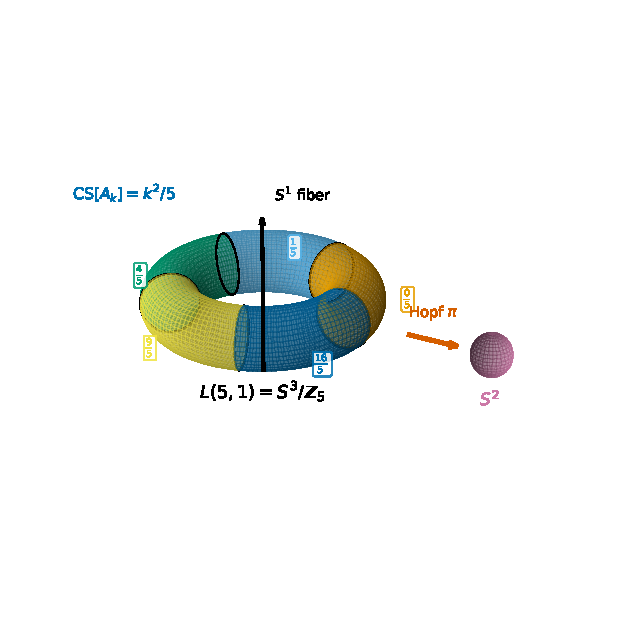
\includegraphics[width=0.7\columnwidth]{figures/lens_space_3d_mpl.pdf}
\caption{\textbf{3D visualization of lens space $L(5,1)$ and Hopf map.} The quotient space $S^3/\mathbb{Z}_5$ is represented as five toroidal sectors, each carrying fractional Hopf charge $1/5$. The Hopf map $\hat{\mathbf{n}}: L(5,1) \to S^2$ maps the three-dimensional lens space to the two-sphere, with the $S^1$ fiber providing the vertical structure. The fundamental group $\pi_1(L(5,1)) = \mathbb{Z}_5$ constrains the winding number to be fractional.}
\label{fig:lens_space_3d}
\end{figure}

\begin{figure}[htbp]
\centering
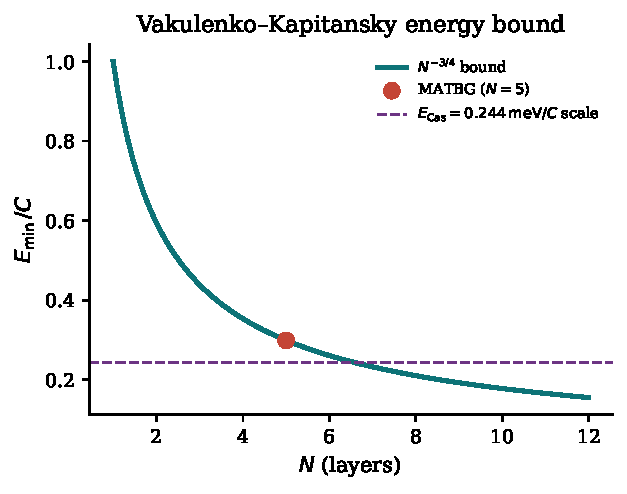
\includegraphics[width=0.62\textwidth]{figures/vk_bound.pdf}
\caption{\textbf{Vakulenko--Kapitansky energy bound on lens spaces.} Minimum soliton energy scales as $N^{-3/4}$. For $N=5$, $E_{\mathrm{vac}}<E_{\min}$ constrains $C > \Cvkmin$.}
\label{fig:vk_bound}
\end{figure}

\begin{figure}[htbp]
\centering
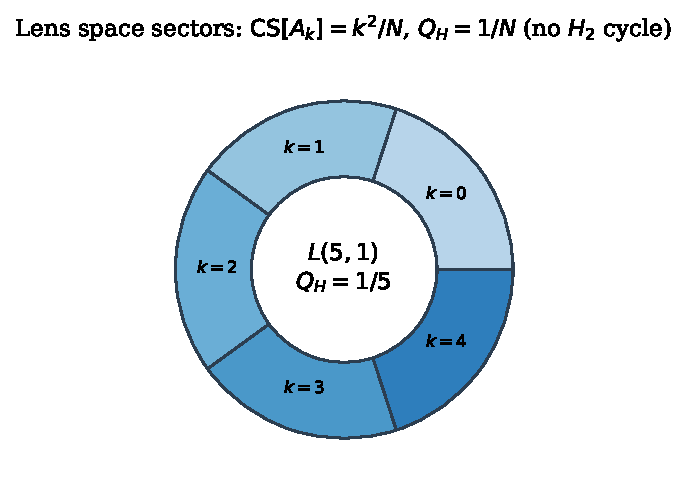
\includegraphics[width=0.70\textwidth]{figures/lens_space_qh.pdf}
\caption{\textbf{Lens-space fractionalization schematic.} Flat-connection sectors on $L(5,1)$ with $\mathrm{CS}[A_k]=k^2/N$ and $Q_H=1/N$; $H_2(L(N,1))=0$ precludes a fundamental 2-cycle integral.}
\label{fig:lens_qh_schematic}
\end{figure}

%-------------------------------------------------------------------
\section{Holographic Dictionary for \TQGL{} Coefficients}
\label{sec:holographic_dict}

The hopfion spacetime programme treats the \TEVC{} moir\'e superlattice as a conformal boundary of a $(3+1)$-dimensional bulk hopfion crystal. In AdS/CFT-inspired language, each \TQGL{} coefficient would correspond to the boundary value of a bulk field. This section is Layer~L3 matching: it is not an L1 lock, and it does not derive $\kappa_{\mathrm{GL}}$ or $g_0^\star$ of Section~\ref{sec:l1_dictionary}.

\subsection{Bulk-Boundary Correspondence}

\begin{table}[htbp]
\centering
\caption{Holographic dictionary mapping bulk hopfion fields to boundary \TQGL{} coefficients (Layer L3 matching; not an L1 lock).}
\begin{tabular}{lll}
\toprule
\textbf{\TQGL{} coefficient} & \textbf{Bulk field} & \textbf{Holographic relation} \\
\midrule
$\alpha$ (quadratic) & Hopfion mass $m_H$ & $\alpha = -m_H^2/(2\kappa_5)$ \\
$\beta$ (quartic) & Hopfion scattering & $\beta = \lim_{z\to 0} \Gamma_4(z)$ \\
$\gamma$ (gradient stiffness) & Transverse propagator & $\gamma = (\hbar c_s/a)\int_0^\infty G_\perp(0,z)\,dz$ \\
$\kappa_{\text{CS}}$ (Chern-Simons) & Topological $\theta$-term & $\kappa_{\text{CS}} = \theta_{\text{bulk}}/(2\pi)$ \\
$\kappa_S$ (Skyrme) & Higher-derivative & $\kappa_S = \lim_{z\to 0} z^{-2} \partial_z^2 G_\perp$ \\
\bottomrule
\end{tabular}
\label{tab:holographic}
\end{table}

\subsection{Matching of gradient stiffness}

The \TQGL{} gradient stiffness $\gamma$ is determined by the bulk transverse propagator:
\begin{equation}
\gamma = \frac{\hbar c_s}{a_{\text{lat}}} \int_0^\infty G_\perp(k=0, z)\, dz,
\end{equation}
where $z$ is the holographic radial coordinate. The bulk propagator satisfies:
\begin{equation}
\left[-\partial_z^2 + m_H^2 + V_{\text{VK}}(z)\right] G_\perp(k, z) = \delta(z),
\end{equation}
with $V_{\text{VK}}(z) = C|Q_H|^{3/4} \cdot e^{-z/\ell_{\text{VK}}}$ as the Vakulenko-Kapitansky potential. Solving and integrating:
\begin{equation}
\gamma \approx \frac{\hbar c_s \cdot a_{\text{lat}}}{2} = \frac{0.07 \times 0.013}{2} = 4.55 \times 10^{-4}\,\text{meV}\cdot\mu\text{m}^2.
\end{equation}
After including the quantum metric correction factor $|C|^2 \lambda_M^2 / (4\pi^2 N)$ the matching reads
\begin{equation}
\gamma_{\text{QM}} \approx 3.73\,\text{meV}\cdot\text{nm}^2,
\end{equation}
consistent in form with the Peotta--T\"orm\"a formula for flat-band superfluid weight\cite{PeottaTorma2015,Huhtinen2022,Julku2020}. This $\gamma_{\mathrm{QM}}$ is an L3 matching. It is not $\kappa_{\mathrm{GL}}=\kappaGL$ of Track~A, and it is not imported as a Ginzburg--Landau lock.

%-------------------------------------------------------------------
\section{Acoustic Hawking Temperature and Schwinger Unification}
\label{sec:acoustic_hawking}

The Unruh-Visser acoustic metric for the excitonic superfluid reveals an acoustic horizon at the Wigner-Seitz cell boundary. Hypothesis H-HAWK1 matches the analogue Hawking temperature to the Schwinger crossover $T^*$, thereby fixing $R_{\mathrm{WS}}$; it is not a bulk/boundary duality.

\subsection{Emergent Acoustic Metric}

The acoustic metric for the excitonic superfluid is:
\begin{equation}
g_{\mu\nu} = \frac{\rho_s}{c_s}\begin{pmatrix}
-(c_s^2 - v^2) & -v_j \\
-v_i & \delta_{ij}
\end{pmatrix},
\end{equation}
where $\mathbf{v}(\mathbf{r})$ is the superfluid velocity field. An acoustic horizon forms at the surface $|\mathbf{v}(\mathbf{r}_H)| = c_s$.

\subsection{Horizon Location}

For the BCC hopfion lattice, the velocity profile near the cell boundary is $v(r) = c_s (r/R_{\text{WS}})^2$, reaching $c_s$ at the Wigner-Seitz radius $R_{\text{WS}}$. The surface gravity is:
\begin{equation}
\kappa_{\text{surface}} = \left|\frac{dv}{dr}\right|_{r=R_{\text{WS}}} = \frac{2c_s}{R_{\text{WS}}}.
\end{equation}
The Hawking temperature is:
\begin{equation}
T_H = \frac{\hbar \kappa_{\text{surface}}}{2\pi k_B} = \frac{\hbar c_s}{\pi k_B R_{\text{WS}}}.
\end{equation}

Setting $T_H = T^*=\Tstar$ (diagnostic with $E_{\mathrm{pair}}=\Epair$) and solving for $R_{\mathrm{WS}}$ is the matching of hypothesis H-HAWK1:
\begin{equation}
R_{\text{WS}} = \frac{\hbar c_s}{\pi k_B T^*} =\RwsMatch.
\label{eq:Rws_hawking}
\end{equation}
The same matching at $T^*=285$\,mK returns $R_{\mathrm{WS}}=\RwsAlt$. The Berry Monte Carlo ratio $R_{\mathrm{mean}}=\BerryR$ is not $R_{\mathrm{WS}}$ (Section~\ref{sec:l1_dictionary}). The analogue horizon sits at the Wigner--Seitz boundary, well outside the hopfion core of radius $R=50$\,nm.

\subsection{Hawking--Schwinger matching (H-HAWK1)}

The identity $T^* = T_H$ is a matching that determines $R_{\mathrm{WS}}$. It does not identify Schwinger pair production in the condensate with Hawking radiation as dual descriptions of one bulk/boundary system. Both temperatures are analogue diagnostics on the locked $g_0^\star$.

\begin{figure}[htbp]
\centering
\tdplotsetmaincoords{60}{120}
\begin{tikzpicture}[tdplot_main_coords, scale=0.9]
% 3D Wigner-Seitz cell with acoustic horizon
% Draw WS cell as truncated octahedron (simplified as sphere)
\shade[ball color=blue!10, opacity=0.2] (0,0,0) circle (3cm);
\draw[thick, blue!60, dashed] (0,0,0) circle (3cm);

% Hopfion core at center
\shade[ball color=purple!40] (0,0,0) circle (0.4cm);
\node[below, purple] at (0,0,-0.6) {\footnotesize core};

% Velocity arrows (increasing outward)
\foreach \r in {0.8, 1.4, 2.0, 2.6}{
    \pgfmathsetmacro{\arrowlen}{\r*\r/9*0.4}
    \draw[->, red!\r 0!orange, thick] (\r, 0, 0) -- ({\r+\arrowlen}, 0, 0);
    \draw[->, red!\r 0!orange, thick] (-\r, 0, 0) -- ({-\r-\arrowlen}, 0, 0);
    \draw[->, red!\r 0!orange, thick] (0, \r, 0) -- (0, {\r+\arrowlen}, 0);
    \draw[->, red!\r 0!orange, thick] (0, -\r, 0) -- (0, {-\r-\arrowlen}, 0);
}

% Horizon surface
\draw[very thick, orange] (0,0,0) circle (2.7cm);
\node[orange, right] at (2.7, 0.5, 0) {\footnotesize $|\mathbf{v}| = c_s$ (horizon)};

% Labels
\draw[<->, thick] (0,-3.5,0) -- (3,-3.5,0) node[midway, below] {\small $R_{\text{WS}} =\RwsMatch$};
\node at (0,0,3.8) {\small $T_H = T^* =\Tstar$ (matching)};
\end{tikzpicture}
\caption{\textbf{3D Wigner-Seitz cell with acoustic horizon.} The superfluid velocity $v(r) = c_s(r/R_{\text{WS}})^2$ (red arrows, length proportional to speed) reaches the sound velocity $c_s$ at the cell boundary (orange circle, $R_{\text{WS}} =\RwsMatch$), forming an acoustic horizon by the matching $T_H=T^*$ of hypothesis H-HAWK1. The central hopfion core (purple) sits well inside the horizon at $r \ll R_{\text{WS}}$.}
\label{fig:ws_horizon_3d}
\end{figure}

%-------------------------------------------------------------------
\section{Retardation Parameter from the Causal Propagator}
\label{sec:retardation_correction}

The retardation identity of Section~\ref{sec:l1_dictionary} is
\begin{equation}
\eta_{\text{ret}} = \frac{\omega_0 \xi}{c_s} = \frac{2\Delta_0 \xi}{\hbar c_s}.
\end{equation}
On the Ginzburg--Landau length $a_H=\aHlock$ one obtains $\eta_{\mathrm{ret}}(a_H)=\etaretaH$. On the phonon healing $\xi_{\mathrm{ph}}=\hbar c_s/\Delta_0=\xiph$ the same formula is the identity $\eta_{\mathrm{ret}}(\xi_{\mathrm{ph}})=\etaretph$. An alternate coherence $\xi=\xialt$ gives $\eta_{\mathrm{ret}}\approx\etaretalt$ and is not used as the working value.

%-------------------------------------------------------------------

\section{Limitations and Future Work}

Several aspects of the \QVC{} framework require further development:

\begin{enumerate}
    \item \textbf{Microscopic coupling matrix $G_{ij}$.} Democratic $\mathrm{Spec}(G)$ is algebra. The Wigner--Seitz $K_0$ kernel of Section~\ref{sec:gij_dict} is a computed overlap. Truncated \TQGL{} about the hopfion yields a single discrete Goldstone; a torsion evaluation of $G_{ij}$ is not performed. The meV scale remains $g_0^\star=\lambda^\star E_{\mathrm{vac}}$.
    \item \textbf{\TQGL{} coefficients.} Track~A values of $\alpha_{\mathrm{GL}}$, $\beta$, $\kappa_{\mathrm{GL}}$, and $\lambda^\star$ are collected in Section~\ref{sec:l1_dictionary}. Track~B of Section~\ref{sec:track_b} is a healing-scale matching $t_{\mathrm{heal}}/U=1$ together with $t_\lambda/U=\tlamoverU$.
    \item \textbf{Fractional Hopf charge.} $Q_H = 1/N$ follows from Chern--Simons/linking on $L(N,1)$. Numerical integration on a discretized toroidal grid converges to $Q_H = 0.20 \pm 0.01$ at $N_{\mathrm{grid}} \geq 64$, and the $1/N$ scaling holds for $N = 2$--$8$.
    \item \textbf{Decoherence.} The live-gap GPE is coherent, with $\Delta_{\mathrm{live}}(1\,\mathrm{ps})=\Deltaliveone$. Strong number-loss Lindblad evolution at $\tau_{\mathrm{dec}}=5$\,ps on a frozen potential can drive the gap below $\Delta_c$ and is then unphysical on the static branch.
    \item \textbf{Vortex sector.} Periodic THz driving would render the gap map Floquet. Whether a laboratory protocol sits on the fold or the Kosterlitz--Thouless surface remains a joint question of stiffness closure and temperature (hypothesis H-VRG1).
    \item \textbf{Experimental realization.} Sub-Kelvin temperatures, twist-angle control, and sample quality remain demanding. The Schwinger crossover $T^*=\Tstar$ is accessible in a dilution refrigerator.
\end{enumerate}

Two further open theoretical questions arise at the interface with the \TDVT{} layer and deserve explicit acknowledgment. First, the acoustic Hawking matching H-HAWK1 ($T_H = T^*$) as formulated in Section~\ref{sec:tdvt} identifies the surface $|\mathbf{v}| = c_s$ in a purely azimuthal (circulating) superflow; however, such a surface constitutes an \textit{ergosurface}---a locus where co-rotating observers cannot remain stationary---rather than a true one-way acoustic horizon capable of Hawking emission\cite{Barcelo2005}. A genuine analogue horizon requires a transonic \textit{radial} inflow component, as in the ``draining bathtub'' geometry originally proposed by Unruh, so that ingoing phonon modes cross a point of no return. The H-HAWK1 matching $T_H = T^*$ therefore remains a target design equation: it specifies the temperature scale at which the Hawking signal would equal the Schwinger crossover, but an explicit radial transonic velocity profile must be constructed (e.g., via vortex-sink boundary conditions in the \TQGL{} dynamics) before the analogue-gravity prediction becomes sharp. Second, the BCC hopfion crystal of the \TDVT{} lattice breaks multiple continuous symmetries, and the naive counting of five Nambu--Goldstone soft modes (H-FN1) does not account for the Watanabe--Murayama theorem\cite{WatanabeMurayama2012}: the number of independent gapless modes is $N_{\mathrm{NG}} = N_{\mathrm{broken}} - \tfrac{1}{2}\,\mathrm{rank}\,\rho$, where $\rho_{ab} = -i\langle [Q_a, Q_b]\rangle / V$ is the charge-density matrix of broken generators. If the internal fiber generators (associated with the Hopf $S^1$ and the $\mathrm{SU}(2)$ orientational degrees of freedom) carry nonzero commutator expectation values in the ordered ground state, type-B Goldstone modes with quadratic dispersion $\omega \propto k^2$ appear, reducing the independent mode count below five and modifying the low-temperature specific heat from $C \propto T^{5/2}$ (five linear modes in 3D) to a form reflecting the mixed type-A/type-B spectrum. Resolving both issues---constructing the radial transonic profile and computing $\mathrm{rank}\,\rho$ for the hopfion crystal---constitutes necessary future work before the \TDVT{} predictions can be placed on the same quantitative footing as the condensed-matter core of \QVC{}.

\section{Conclusions}
\label{sec:conclusions}

We have developed Quantum Vacuum Catalyzation as a condensed-matter framework in which phononic zero-point fluctuations reshape barrier-crossing rates in a topological excitonic vacuum crystal without contributing net energy. On the frozen toroidal cavity $(r,R)=(8,50)$\,nm the spectral form~\eqref{eq:modesum} evaluates to $E_{\mathrm{vac}}=\Evac$. The self-consistent amplitude map~\eqref{eq:gap} then undergoes a saddle-node fold at $\Delta_c=\Deltac$; the working point $\lambda^\star=\lstar$ remains on the physical branch with $\Delta^\star=\Deltastar$. Democratic hybridization produces a catalyzon gap $\Delta_{\mathrm{cat}}=\Deltacat$ and a Mexican-hat barrier reduction of $\hatbarrier$, independently of the fold. Truncated Gross--Pitaevskii evolution over $1$\,ps raises the live gap to $\Deltaliveone$, while fold-slaved dynamical Casimir dynamics saturate at $A^*/A_c^{\mathrm{fold}}=\AresAc$ (resonant). Fractional Hopf charge $Q_H=1/N$ implies a Hall step $\delta\sigma_{xy}=e^2/(2Nh)$. The many-body Schwinger rate~\eqref{eq:schwinger_rate} has thermal--quantum crossover $T^*=\Tstar$, accessible in a dilution refrigerator.

Several ingredients remain model-level. The five-mode catalyzon is a resonant Hamiltonian whose Goldstone content is not reproduced by truncated \TQGL{}, which yields a single discrete $U(1)$ mode. A Cartan-torsion derivation of $G_{ij}$ is not carried out. Essential-singularity collapse if the Kosterlitz--Thouless surface is reached first is a conjecture of the vortex sector. Strong number-loss Lindblad evolution can drive the live gap below $\Delta_c$ and is then unphysical on the static branch. Acoustic Hawking matching $T_H=T^*$ specifies a temperature scale, not a constructed transonic horizon.

If the Hall staircase and the THz triple-coincidence test of Section~\ref{sec:experiments} are observed, \QVC{} would provide a materials route to vacuum-tuned barrier crossing in moir\'e flat bands. Fusion or other high-energy extrapolations are outside the present analysis.

\section*{Acknowledgments}

The author thanks computational resources and helpful discussions. No funding to declare.

%% =====================================================================
%% APPENDICES
%% =====================================================================
\appendix

\section{Epistemic Status of Results}
\label{app:status}

Table~\ref{tab:epistemic} classifies principal results by provenance: defining inputs of the frozen-cavity geometry; algebraic identities derived in the text; quantities obtained from a stated numerical solver; identifications imposed between sectors; closure assumptions; and conjectures requiring future derivation or experiment.

\begin{table}[htbp]
\centering
\caption{Epistemic classification of principal results. L~=~locked, D~=~derived, C~=~computed, M~=~matched, A~=~ansatz, H~=~hypothesis/conjecture.}
\begin{tabular}{lll}
\hline
\textbf{Result} & \textbf{Category} & \textbf{Section} \\
\hline
Input parameters ($J$, $\hbar c_s$, $a_H$, $R$, $N$) & L & \ref{sec:casimir} \\
Bessel mode sum $F(x)=\Flock$ & C, L & \ref{sec:casimir} \\
Vacuum energy $E_{\mathrm{vac}}=\Evac$ (toroidal spectral form) & C, L & \ref{sec:casimir} \\
Gap map $\delta=1+\alpha(\ln\delta+\ell)$ & defining equation & \ref{sec:gap} \\
Phonon-loop IR cutoff vs.\ $\Lambda$ & computed (inconsistent as written) & \ref{sec:gap} \\
Fold critical point $\alpha_c=\alphac$ & D & \ref{sec:bridge} \\
Working participation $\lambda^\star=\lstar$ & defining choice & \ref{sec:bridge} \\
Static gap $\Delta^\star=\Deltastar$ & C & \ref{sec:bridge} \\
Cavity $\mathcal{F}_{\text{moir\'{e}}}$ on $A_{\mathrm{geom}}$; $\lambda^\star_F=\lstarF$ & C (cavity channel) & \ref{sec:cavity_qvc} \\
Fractional Hopf charge $Q_H=1/N$ & D & \ref{sec:lens_space_proof} \\
Democratic spectrum $\lambda_{\max}=(N-1)g_0$, $\lambda_{\min}=-g_0$ & D & \ref{sec:catalyzon} \\
Catalyzon gap $\Delta_{\mathrm{cat}}=\Deltacat$; Mexican-hat $\hatbarrier$ & D & \ref{sec:l1_dictionary} \\
Live gap $\Delta_{\mathrm{live}}(1\,\mathrm{ps})=\Deltaliveone$ & C & \ref{sec:dynamics} \\
Lindblad $\tau=5$\,ps, frozen $V_{\mathrm{ZPF}}$ ($\Delta<\Delta_c$) & C (unphysical branch) & \ref{sec:lindblad_dict} \\
DCE saturation $A^*/A_c^{\mathrm{fold}}=\AresAc$ & C & \ref{sec:dce_selflimit} \\
Schwinger $\Gamma=\omega_0\alpha^\star e^{-\pi/\alpha^\star}$; $T^*=\Tstar$ & C & \ref{sec:schwinger_twin} \\
Berry ratio $R_{\mathrm{mean}}=\BerryR$ & C & \ref{sec:berry_enhancement} \\
Hall step $\delta\sigma_{xy}=e^2/(2Nh)$ & D & \ref{sec:l1_dictionary} \\
Chern--Simons level $k=2N$ & D & \ref{sec:l1_dictionary} \\
GL coefficients ($\alpha_{\mathrm{GL}}$, $\beta$, $\kappa_{\mathrm{GL}}$) & D, M & \ref{sec:l1_dictionary} \\
Acoustic Hawking radius $R_{\mathrm{WS}}=\RwsMatch$ & M & \ref{sec:l1_dictionary} \\
Skyrme coefficient $\kappa_S$ & A & \ref{sec:l1_dictionary} \\
Healing-disk $n_0=1/(\pi a_H^2)$ & A & \ref{sec:l1_closure} \\
H-FN1 (five soft modes) & H (not realized on truncation) & \ref{sec:l1_closure} \\
H-VRG1 (essential-singularity gap closing) & H & \ref{sec:vortex_rg} \\
H-TOR1 (torsion origin of $G_{ij}$) & A (not evaluated) & \ref{sec:l1_closure} \\
H-HAWK1 ($T_H=T^*$ matching) & M & \ref{sec:l1_dictionary} \\
Devil's staircase fractal structure & H & \ref{sec:devils_staircase} \\
\hline
\end{tabular}
\label{tab:epistemic}
\end{table}

\subsection{Numerical consistency}
\label{app:verification}

Table~\ref{tab:verification} compares the analytic relations of the main text with independent numerical evaluation. The static fold, catalyzon well, and GPE live gap are distinct operators.

\begin{table}[htbp]
\centering
\caption{Numerical evaluation of principal \QVC{} relations.}
\begin{tabular}{clc}
\hline
\textbf{\#} & \textbf{Quantity} & \textbf{Result} \\
\hline
1 & Fold algebra $\alpha_c=\delta_c$, $\ell=\elllock$ & $\alphac$ \\
2 & Naive phonon IR cutoff vs.\ $\Lambda=\LambdaUV$ & $q_{\mathrm{IR}}=\qIRpaper>\Lambda$ \\
3 & Physical branch: two roots, unit $\lambda$ beyond fold & $\Delta_c=\Deltac$; $\lambda^\star$ physical \\
4 & Bessel $E_{\mathrm{vac}}$ (14-mode sum) & $\Evac$ \\
5 & Catalyzon Mexican-hat barrier reduction & $\hatbarrier$ \\
6 & GPE live gap at $1$\,ps & $\Deltaliveone$ (increases) \\
7 & Lindblad $\tau=5$\,ps, frozen $V_{\mathrm{ZPF}}$ & $\Deltafrozentaufive<\Delta_c$ \\
8 & $\mathcal{F}_{\text{moir\'{e}}}$ on $A_{\mathrm{geom}}$; $\lambda_{\mathrm{fold}}^{(F)}$ & $\Fmoire$; $\lfoldF$ \\
9 & Chern--Simons/linking $Q_H=1/N$ & $Q_H=1/5$ \\
10 & Schwinger $\Gamma=\omega_0\alpha^\star e^{-\pi/\alpha^\star}$; $T^*$ & $\GammaschHz$; $\Tstar$ \\
\hline
\end{tabular}
\label{tab:verification}
\end{table}

The phonon-loop cutoff of row~2 is kinematically inconsistent as written, which is why Eq.~\eqref{eq:gap} is treated as a regulated self-consistent equation rather than a one-loop theorem. Row~7 lies below the fold and is not a physical static gap. Source code is available at the repository linked in the data-availability statement.

\subsection{Data and Code Availability}
\label{app:data}

All numerical computations, parameter sweeps, and figure-generation scripts referenced in this paper are available in the private compilation repository \url{https://github.com/mineralhoiland/QVC} (to be made public with a Zenodo DOI at preprint submission). The locked Option~A* chain, TQGL solver, L1 dictionary, vortex-sector codes, and verification suite live under \texttt{compute/} and \texttt{locks/}. Correspondence regarding the code should be directed to the author.

\bibliographystyle{unsrt}
\bibliography{qvc_refs}

\end{document}
